%\documentclass[journal]{vgtc}                % final (journal style)
\documentclass[review,journal]{vgtc}          % review (journal style)
%\documentclass[widereview]{vgtc}             % wide-spaced review
%\documentclass[preprint,journal]{vgtc}       % preprint (journal style)
%\documentclass[electronic,journal]{vgtc}     % electronic version, journal

%% Uncomment one of the lines above depending on where your paper is
%% in the conference process. ``review'' and ``widereview'' are for review
%% submission, ``preprint'' is for pre-publication, and the final version
%% doesn't use a specific qualifier. Further, ``electronic'' includes
%% hyperreferences for more convenient online viewing.

%% Please use one of the ``review'' options in combination with the
%% assigned online id (see below) ONLY if your paper uses a double blind
%% review process. Some conferences, like IEEE Vis and InfoVis, have NOT
%% in the past.

%% Please note that the use of figures other than the optional teaser is not permitted on the first page
%% of the journal version.  Figures should begin on the second page and be
%% in CMYK or Grey scale format, otherwise, colour shifting may occur
%% during the printing process.  Papers submitted with figures other than the optional teaser on the
%% first page will be refused.

%% These three lines bring in essential packages: ``mathptmx'' for Type 1
%% typefaces, ``graphicx'' for inclusion of EPS figures. and ``times''
%% for proper handling of the times font family.

\usepackage{mathptmx}
\usepackage{psfrag}
\usepackage{graphicx}
\usepackage{epstopdf}
\usepackage{times}

\usepackage{amssymb,amsmath,amsthm}
\usepackage[lined,linesnumbered]{algorithm2e}
\usepackage{caption}
\usepackage{subcaption}
\usepackage{multirow}
\usepackage{framed}
\usepackage{tikz}
\usepackage{array}
\usepackage{xypic}

%% We encourage the use of mathptmx for consistent usage of times font
%% throughout the proceedings. However, if you encounter conflicts
%% with other math-related packages, you may want to disable it.

%% This turns references into clickable hyperlinks.
\usepackage[bookmarks,backref=true,linkcolor=black]{hyperref} %,colorlinks
\hypersetup{
  pdfauthor = {},
  pdftitle = {},
  pdfsubject = {},
  pdfkeywords = {},
  colorlinks=true,
  linkcolor= black,
  citecolor= black,
  pageanchor=true,
  urlcolor = black,
  plainpages = false,
  linktocpage
}

%% If you are submitting a paper to a conference for review with a double
%% blind reviewing process, please replace the value ``0'' below with your
%% OnlineID. Otherwise, you may safely leave it at ``0''.
\onlineid{0}

%% declare the category of your paper, only shown in review mode
\vgtccategory{Technique}

%% allow for this line if you want the electronic option to work properly
\vgtcinsertpkg

%% In preprint mode you may define your own headline.
%\preprinttext{To appear in an IEEE VGTC sponsored conference.}


%%%%%%%%%%%%%%%%%%%%%%%%%%%%%%%%%%%%%%%%%%%%%%%%%%%%%%%%%%%%%%%%%%%%%%%%%%%%%
%
% Math commands
%
%%%%%%%%%%%%%%%%%%%%%%%%%%%%%%%%%%%%%%%%%%%%%%%%%%%%%%%%%%%%%%%%%%%%%%%%%%%%%

\newcommand {\emath}[1]  {\ensuremath{#1}}
\newcommand {\R}         {\emath{\mathbb{R}}}        % Real space
\newcommand {\Real}[1]   {\emath{\mathbb{R}^{#1}}}   % Real space
\newcommand {\Rd}        {\Real{d}}                  % R^d
\newcommand {\Rdone}     {\Real{d+1}}                % R^d+1
\newcommand {\Rk}        {\Real{k}}                  % R^k
\newcommand {\Rtwo}      {\Real{2}}                  % R^2
\newcommand {\Rthree}    {\Real{3}}                  % R^3
\newcommand {\Rfour}     {\Real{4}}                  % R^4
\newcommand {\Sphere}[1] {\emath{\mathbb{S}^{#1}}}   % Sphere
\newcommand {\Sk}        {\Sphere{k}}                % S^k
\newcommand {\Sd}        {\Sphere{d}}                % S^d
\newcommand {\BB}        {\emath{\mathbb{B}}}        % B
\newcommand {\Ball}[1]   {\emath{\mathbb{B}^{#1}}}   % B^{#1}
\newcommand {\Ballep}    {\emath{B^{\epsilon}_{p}}}  % B^e_p
\newcommand {\cl}        {\emath{\mathrm{cl}}}       % cl
\newcommand {\cb}        {\emath{\mathbf{c}}}        % bold c
\newcommand {\tcb}       {\emath{{\tilde{\cb}}}}     % bold c~
\newcommand {\eb}        {\emath{\mathbf{e}}}        % bold e
\newcommand {\tpi}       {\emath{\tilde{\pi}}}       % \pi~
\newcommand {\gDim}[1]   {\emath{#1 \times #1 \times #1}} % DxDxD

\newcommand {\tg}        {\emath{\tilde{g}}}
\newcommand {\tn}        {\emath{\tilde{n}}}
\newcommand {\tw}        {\emath{\tilde{w}}}
\newcommand {\IV}        {\emath{\mathcal{I_V}}}
\newcommand {\Orth}      {\emath{\mathcal{O}}}
\newcommand {\hN}        {\emath{\widehat{N}}}
\newcommand {\pinvA}     {\emath{\tilde{A}^{-1}}}
\newcommand {\XX}        {\emath{\mathcal{X}}}
\newcommand {\Ccorner}   {C_{\mathrm{corner}}}       % C_corner
\newcommand {\Cedge}     {C_{\mathrm{edge}}}         % C_edge
\newcommand {\Cselected} {C_{\mathrm{selected}}}     % C_selected
\newcommand {\RIII}      {\emath{R^{\gDim{3}}}}      % R^{3x3x3}
\newcommand {\RV}        {\emath{R^{\gDim{5}}}}      % R^{5x5x5}
\newcommand {\hRV}       {\emath{\widehat{R}^{\gDim{5}}}} % Rhat^{5x5x5}

\newtheorem{proposition}{Proposition}
\newtheorem{corollary}{Corollary}[proposition]
\newtheorem{lemma}[proposition]{Lemma}


% xypic commands for drawing flowcharts
\newcommand {\action}[1] {*+[F] \txt{#1}}
\newcommand {\laction}[1] 
  {*+[F] \txt{\mbox{\setlength{\tabcolsep}{0pt}
                    \begin{tabular}{l}#1\end{tabular}}}}

%%%%%%%%%%%%%%%%%%%%%%%%%%%%%%%%%%%%%%%%%%%%%%%%%%%%%%%%%%%%%%%%%%%%%%%%%%%%%
%
% tikz block styles
%
%%%%%%%%%%%%%%%%%%%%%%%%%%%%%%%%%%%%%%%%%%%%%%%%%%%%%%%%%%%%%%%%%%%%%%%%%%%%%

\usetikzlibrary{shapes,arrows}

\tikzstyle{action} = [rectangle, draw, text centered, node distance=4cm, minimum height=4em]
\tikzstyle{source} = [draw, ellipse, text centered, node distance=1.5cm, minimum height=4em, text width=3cm]
\tikzstyle{sink} = [draw, ellipse, text centered, node distance=2cm, minimum height=4em]
\tikzstyle{line} = [draw, -latex']
\tikzstyle{figlabel} = [text centered, node distance=1.5cm, text width=1cm]

%%%%%%%%%%%%%%%%%%%%%%%%%%%%%%%%%%%%%%%%%%%%%%%%%%%%%%%%%%%%%%%%%%%%%%%%%%%%%
%
% algorithm2e keywords and commands
%
%%%%%%%%%%%%%%%%%%%%%%%%%%%%%%%%%%%%%%%%%%%%%%%%%%%%%%%%%%%%%%%%%%%%%%%%%%%%%

% algorithm2e global keywords
\SetKw{Function}{Function}
\SetKw{true}{true}
\SetKw{false}{false}
\SetKw{KwAnd}{and}
\SetKw{KwOr}{or}
\SetKw{true}{true}
\SetKw{false}{false}
\SetKw{KwElse}{else}
\SetKw{KwDownTo}{downto}
\SetKwData{NULL}{NULL}
\SetKwInOut{Input}{Input}
\SetKwInOut{Output}{Output}
\SetKwInOut{Result}{Result}
\SetKwInOut{Requires}{Requires}
\ResetInOut{Requires1}
\SetKwComment{NoLineNum}{}{}
\SetCommentSty{textit}
\SetArgSty{textrm}
\SetFuncSty{textsc}
\SetAlgoLined

\IncMargin{1ex}

\SetKwFunction{AngleTest}{AngleTest}
\SetKwFunction{ScalarTest}{ScalarTest}
\SetKwFunction{ReliableGrad}{ReliableGrad}
\SetKwFunction{MergeSharp}{MergeSharp}
\SetKwFunction{FindSharp}{FindSharp}
\SetKwFunction{CountDegree}{CountDegree}
\SetKwFunction{SelectiveFindSharp}{SelectiveFindSharp}
\SetKwFunction{Magnitude}{Magnitude}
\SetKwFunction{Angle}{Angle}
\SetKwFunction{Distance}{Distance}
\SetKwData{Grid}{Grid}
\SetKwData{numAgree}{numAgree}
\SetKwData{errorDist}{errorDist}
\SetKwData{maxErrorDist}{maxErrorDist}
\SetKwData{numIter}{numIter}

% Algorithm function names and variables
\SetKwFunction{DoesOrthMatch}{DoesOrthMatch}
\SetKwFunction{DoesOrthMatchA}{DoesOrthMatchA}
\SetKwFunction{DoesOrthMatchB}{DoesOrthMatchB}
\SetKwFunction{ExtendReliable}{ExtendReliable}


\SetKwData{Center}{Center}
\SetKwData{Centroid}{Centroid}
\SetKwData{centroid}{centroid}
\SetKwData{isov}{isov}
\SetKwData{isovLoc}{isovLoc}
\SetKwData{numLargeEigenvalues}{numLargeEigenvalues}

% algorithm2e reset line number
\newcommand {\ResetAlgoLineNumber} {\setcounter{AlgoLine}{0}}

\SetAlgoCaptionSeparator{.}


%%%%%%%%%%%%%%%%%%%%%%%%%%%%%%%%%%%%%%%%%%%%%%%%%%%%%%%%%%%%%%%%%%%%%%%%%%%%%
%
% psfrag commands
%
%%%%%%%%%%%%%%%%%%%%%%%%%%%%%%%%%%%%%%%%%%%%%%%%%%%%%%%%%%%%%%%%%%%%%%%%%%%%%

\psfrag{a}{$\alpha$}
\psfrag{n}{$n_v$}
\psfrag{np}{$n_{v'}$}
\psfrag{tn}{$\tn_v$}
\psfrag{tnp}{$\tn_{v'}$}
\psfrag{phi}{$\phi(n_v,n_{v'})$}
\psfrag{phi2}{$\phi_2(n_v,n_{v'})$}
\psfrag{phitn}{$\phi(\tn_v,n_{v'})$}
\psfrag{phitnp}{$\phi(n,\tn_{v'})$}



\title{SHREC: Sharp reconstruction of isosurfaces}

%% This is how authors are specified in the journal style

%% indicate IEEE Member or Student Member in form indicated below
\author{Arindam Bhattacharya, Ross Vasko and Rephael Wenger}
\authorfooter{
The Ohio State University. E-mail: wenger.4@osu.edu, 
vasko.38@buckeyemail.osu.edu, bhattaca@cse.ohio-state.edu}

\abstract{
We present an algorithm, called SHREC,
for constructing isosurfaces with sharp edges and corners.
Algorithm SHREC computes isosurface vertex locations on sharp features,
selects a well-spaced subset of these vertices,
and merges isosurface vertices in the neighborhood of each selected vertex.
The resulting isosurfaces have good representations of sharp features.
Algorithm SHREC is similar to a previous algorithm, MergeSharp,
but improves on MergeSharp
by better generation of isosurface vertices,
better selections of vertices on sharp features
and better choices in merging.
We also define a function to measure the closeness 
of the normals between two surfaces
and use this function to evaluate the quality of reconstructions
of surfaces with sharp features.}

%% Keywords that describe your work. Will show as 'Index Terms' in journal
%% please capitalize first letter and insert punctuation after last keyword
\keywords{Isosurface, sharp features, industrial CT, gradient computation,
line drawings.}

%% ACM Computing Classification System (CCS). 
%% See <http://www.acm.org/class/1998/> for details.
%% The ``\CCScat'' command takes four arguments.

\CCScatlist{ % not used in journal version
\CCScat{I.3.5}{Computer Graphics}{Computational Geometry and Object Modeling}
}

%% Uncomment below to include a teaser figure.
%\teaser{
%}

%% Uncomment below to disable the manuscript note
%\renewcommand{\manuscriptnotetxt}{}

%% Copyright space is enabled by default as required by guidelines.
%% It is disabled by the 'review' option or via the following command:
% \nocopyrightspace

\renewcommand{\textfraction}{0.2}
\renewcommand{\dbltopfraction}{0.8}	
\renewcommand{\topfraction}{0.8}	


%%%%%%%%%%%%%%%%%%%%%%%%%%%%%%%%%%%%%%%%%%%%%%%%%%%%%%%%%%%%%%%%
%%%%%%%%%%%%%%%%%%%%%% START OF THE PAPER %%%%%%%%%%%%%%%%%%%%%%
%%%%%%%%%%%%%%%%%%%%%%%%%%%%%%%%%%%%%%%%%%%%%%%%%%%%%%%%%%%%%%%%%

\begin{document}



\firstsection{Introduction}

\maketitle

Given a regular grid sampling of a scalar field, $f: \Rthree \rightarrow \R$,
and a scalar value $\sigma$,
we are interested in constructing a good mesh representation
of the level set $f^{-1}(\sigma) = \{x : f(x) = \sigma \}$.
Such a representation is called an {\em isosurface} 
and the scalar value $\sigma$ is called an {\em isovalue}.

When $f$ is smooth,
i.e., when $f$ is continuous and its derivatives are continuous,
a number of algorithms do an excellent job of isosurface construction.
However, if the gradient field of $f$ is discontinuous,
then the problem of isosurface construction is more challenging.
If the level set $f^{-1}(\sigma)$ intersects a gradient discontinuity,
then the level set $f^{-1}(\sigma)$ will have a ``sharp corner''
(a 0-dimensional feature) or a ``sharp edge'' (a 1-dimensional feature)
at that discontinuity.
We are interested in constructing isosurfaces
which do a good job of representing those sharp features.

Isosurfaces are represented by piecewise linear or piecewise smooth meshes,
usually composed of triangles or quadrilaterals.
This underlying mesh should model the sharp features
of the isosurface $\Sigma$.
A 1-dimensionalf feature of $\Sigma$ with dihedral angle $\alpha$
should be represented by a single, 
connected sequence of mesh edges with dihedral angle near $\alpha$.
A 0-dimensional feature of $\Sigma$ with solid angle $\alpha$
should be represented by a single
isosurface vertex with solid angle near $\alpha$.
On the other hand, mesh edges and vertices
representing smooth, low curvature portions of $\Sigma$ should have
dihedral angles near 180 degrees and solid angles near $2 \pi$.

A number of algorithms have been proposed
for constructing isosurfaces 
with sharp features~\cite{ab-fpmmo-03,gk-eretm-04,hwco-cmsaf-05,
jlsw-dchd-02,kbsh-fssev-01,ms-ispmg-10,Varadhan:2003:fss,
sw-dmcpc-04,zhk-dctps-04}.
Unfortunately, these algorithms create ``notches'' along sharp edges,
degenerate, zero area triangles or quadrilaterals,
and ``folds'' in the mesh with ``flipped'' triangles.
(See Figures~??? in Section~??? for illustrations of these problems.)

In~\cite{bw-cisec-13},
we describe an algorithm, MergeSharp,
for constructing isosurfaces with sharp features
based on merging grid cubes around sharp features.
By placing a single isosurface vertex in these merged regions,
MergeSharp significantly reduces problems of ``notches'',
degenerate mesh polygons and ``folds'' in the mesh.
While MergeSharp reduced the mesh problems,
it did not eliminate them, 
with many meshes still having
one or two locations with degenerate mesh polygons or folds in the mesh.

In this paper, we present an algorithm, SHREC,
which almost completely eliminates the mesh problems listed above.
The algorithm is based on the MergeSharp paradigm,
where grid cubes around sharp features are merged
into a region containing a single isosurface vertex.
However, it differs from MergeSharp by better generation
of isosurface vertices on sharp features,
better selection of isosurface vertices on the sharp features,
and more controlled merging of grid cubes.
The algorithm performs measurably better
than MergeSharp or than other algorithms for which we had implementations.

There is extensive work on construction of surfaces with sharp features 
from point cloud data,
e.g.~\cite{avron2010L,cdr-drpsc-07,Daniels:2007:Robust,Dey2012,
fcs-rmlsf-2005,Oztireli2009,sym-fpmg-10,Wang:2013:Feature}
and many other articles.
In~\cite{Oztireli2009} and~\cite{Wang:2013:Feature},
the final construction of the surface mesh is accomplished 
by Marching Cubes~\cite{lc-mchr3-87}
or some other isosurface reconstruction algorithm.
The algorithms in this and similar papers
can be used by algorithms in those papers
to construct a surface mesh that better represents sharp surface features
than the Marching Cubes isosurface.

In~\cite{cdr-drpsc-07,Dey2012} and~\cite{sym-fpmg-10},
the final construction of the surface mesh is accomplished
by Voronoi based algorithms described 
in~\cite{cdr-drpsc-07} and \cite{Dey2012}.
These algorithms could be applied to isosurface reconstruction
from regular grid scalar data
by constructing point clouds from the grid data
and then applying the algorithms to the point clouds.
We compare isosurfaces with sharp features constructed
using the algorithm from~\cite{Dey2012}
with isosurfaces constructed by our algorithm.

Few of the isosurface or point cloud reconstruction papers
provide quantitative analysis of the resulting surfaces.
Some provide a distance measure (Hausdorff or root-mean squared)
between the constructed surface and an ideal surface,
but such measures fail to capture errors in surface normals
of the mesh polygons.
Instead of quantitative measures,
most papers provide a few images for visual inspection
of the quality of reconstructed features.
Needless to say, the lack of quantitative measures makes it
difficult evaluate the quality of the algorithms results,
to compare different algorithms,
or to comprehensively test an algorithm on a large number of data sets.

In contrast, the Hausdorff metric and variants are excellent
quantitative measures of the difference between reconstructed
and ideal smooth surfaces.
Software tools such as Metro~\cite{Cignoni:1998:metro} 
and MESH~\cite{Aspert:2002:MESH} are commonly used to measure
the quality of surface reconstructions
and provide quantitative evaluations of reported results.
However, these tools completely ignore surface orientation
and are not suitable for evaluating reconstructed features.

In this paper, we present the angular distance as a measure
of the difference between the surface orientation of two meshes.
Essentially, the angular distance measures the difference 
between the surface normal at a point on one mesh with the surface normals
on nearby points on the other mesh.
The angular distance is defined and discussed
in Section~\ref{section:angular_distance}.
We also provide a software tool which measures the angular distance.

In this paper, we are using the term ``feature'' to refer 
to a ``significant'' discontinuity in surface normals,
not a region with higher curvature.
Most of the papers on reconstruction from point clouds
don't distinguish between discontinuities in surface normals
and surface points with high curvature.
When isosurfaces are reconstructed from scalar data on a regular grid,
the sampling density is fixed and
it is impossible to determine if the original surface has
a discontinuity in surface normals or very high curvature.
Thus, we assume that features in our ideal surface are
points or curves where the surface normal is discontinuous.


\subsection*{Contributions}

The major contibution of our work is an isosurface generation algorithm
called SHREC which does measurable better than previous algorithms
in constructing isosurfaces with sharp features.
In particular, SHREC does better at generating and selecting vertices 
on sharp features and in avoiding constructing degenerate 
or small angle triangles and flipping triangles.
A second contribution is a a definition of the angular distance 
between two surfaces and the application of the angular distance
to evaluate the quality of surface reconstruction algorithms.



\section{Related Work}
\label{section:related}

The well-known Marching Cubes algorithm~\cite{lc-mchr3-87}
by Lorensen and Cline
constructs isosurface patches within active grid cubes.
The isosurface patches align along their common boundaries.
Because Marching Cubes positions vertices only on grid edges,
never inside grid cubes,
it does a poor job at representing sharp features on isosurfaces.

Dual contouring algorithms construct an isosurface using quadrilaterals
which are dual to bipolar grid edges.
The isosurface vertices are located within the grid cubes,
not on grid edges.
Gibson~\cite{gh-ssqem-97,g-cesng-98} gave the first dual contouring algorithm
which she called surface nets.
Because Gibson's algorithm placed only one isosurface vertex 
in each active cube,
it produced many isosurface edges contained in four quadrilaterals.
Thus, the resulting isosurface was not a manifold.
Nielson~\cite{n-dmc-04} modified Gibson's algorithm
to allow multiple isosurface vertices in active cubes.
The number of vertices in a grid cube $\cb$
corresponds to the number of isosurface patches in $\cb$
produced by the Marching Cubes algorithm.

Nielson's algorithm eliminates most, but not all, 
of the non-manifold problems in dual contouring.
A dual contouring algorithm
for constructing an isosurface which is a always a manifold
is contained in~\cite{Wenger:2013:Isosurfaces}.
The algorithm is essentially Nielson's algorithm
but the number and connectivity of isosurface vertices in grid cubes
is sometimes modified.

In~\cite{l-oslpm-00}, Lindstrom gave an algorithm for locating a point 
on a surface from a set of $n$ tangent planes.
The $n$ tangent give a set of $n$ equations in three unknowns,
described by $M x = b$ where $M$ is an $n \times 3$ matrix 
and $b$ is a column vector of length $n$.
Lindstrom uses the singular valued decomposition (SVD) of $M$
to determine a point close to all the tangent planes.
The SVD of $M$ also indicates whether the point is
on a 0-dimensional (corner) or 1-dimensional (edge) surface feature
or on a smooth portion of the surface
Lindstrom's algorithm is described in more detail 
in Section~\ref{section:loc}.
All the papers for isosurface construction with sharp features
use Lindstrom's algorithm or some variation
to locate points on sharp features.
Most of them also use Lindstrom's algorithm to identify sharp features
and classify them as 0 or 1 dimensional.

Kobbelt et al.~\cite{kbsh-fssev-01} modified Marching Cubes 
to position vertices inside grid cubes when those grid cubes
intersected sharp features.
In addition to scalar values at regular grid vertices,
the algorithm by Kobbelt et al. requires a directed distance field
representing the distance along each axis to the modeled surface.
The algorithm uses the directed distance field
to locate points on sharp features.

Ju et al.~\cite{jlsw-dchd-02,sw-dcss-02} present a dual contouring algorithm
for constructing isosurfaces with sharp features.
Vertices of dual contouring isosurfaces lie inside grid cubes
while isosurface quadrilaterals are dual to grid edges.
Dual contouring algorithms were first described
by Gibson in~\cite{gh-ssqem-97,g-cesng-98}.
In addition to scalar values at regular grid vertices,
the algorithm by Ju et al. requires surface normals
at the intersection of the grid edges and the surface.
The surface normals are used to construct tangent planes
intersecting a grid cube.
Ju et al. apply Lindstrom's algorithm to the tangent planes
to locate an isosurface vertex in each grid cube
and determine if the vertex lies on a sharp 0 or 1 dimensional feature.
Variations on~\cite{jlsw-dchd-02} are given 
in~\cite{zhk-dctps-04,Varadhan:2003:fss}.

Ashida and Bandler~\cite{ab-fpmmo-03}, Ho et al.~\cite{hwco-cmsaf-05}
and Gre{\ss} and Klein~\cite{gk-eretm-04} give algorithms
for constructing multiresolution isosurface with sharp features
using oct-trees or kd-trees.
The isosurface mesh is constructed
by first constructing polygonal curves representing the intersection
of the isosurface and oct-tree or kd-tree cells,
and then connecting an isosurface vertex with those polgyonal curves.
As in~\cite{jlsw-dchd-02},
isosurface locations are computed from input surface normals
using Lindstrom's algorithm.

The Dual Marching Cubes\footnote{Nielson also calls his
dual contouring algorithm ``Dual Marching Cubes''~\cite{n-dmc-04},
but it is totally different from Schaefer and Warren's algorithm.}
algorithm by Schaefer and Warren~\cite{sw-dmcpc-04}
constructs a dual mesh which aligns with sharp features
and then extracts the isosurface from that mesh 
using Marching Cubes.
Vertices of the dual mesh are positioned on sharp features
using Lindstrom's algorithm.
Because the isosurface is extracted using Marching Cubes,
the isosurface will have many "sliver" triangles with small angles.
Dual Marching Cubes reduces the number of "sliver" triangles
by positioning the vertices of the dual grid to lie on the isosurface,
whenever possible.

With the exception of~\cite{hwco-cmsaf-05},
none of the reconstruction papers listed above give any quantitative
analysis of the reconstructed features.
Ho et al.~\cite{hwco-cmsaf-05} measured the geometric distance
between the boundary of the union of three random tetrehedra and 
the reconstructed surface produced by their algorithm.
Unfortunately, Ho et al. do not explain whether the geometric distance
is the Hausdorff distance or some distance averaged over the surface.
In any case, they are not measuring the correspondence 
between surface normals.

The algorithms described above 
produce ``sliver'' triangles with very small angles 
along the 1-dimensional features.
A small perturbation of a vertex of such triangles
has a large effect on the triangle normal direction,
so the normal direction of such triangles is almost arbitrary.
The triangle angles may be so small that the triangles are effectively
degenerate with zero area.

With the exception of~\cite{sw-dmcpc-04},
all the algorithms listed above generate isosurface vertices
within active grid cubes.
However, a sharp edge (1-dimensional feature) may intersect 
an inactive grid cube  and a sharp corner (0-dimensional feature) 
may lie in an inactive grid cube.
In such cases, the algorithms produce isosurfaces which contain notches
or truncated corners.
The algorithms could be modified to allow placement of isosurface vertices
in inactive grid cubes,
but at the cost of exacerbating the problem 
of sliver and degenerate triangles.
Placing vertices in inactive grid cubes also introduces a new problem 
of isosurface vertices in the wrong order along 1-dimensional features
creating folds in the mesh.

The MergeSharp algorithm by Bhattaca and Wenger~\cite{bw-cisec-13,bw-erm-13}
attacks the problem of sliver triangles, notches, and folds
by merging grid cubes around features
so that isosurface vertices on features are well-separated 
from each other and from non-feature vertices.
Isosurface vertices are permitted to be placed in inactive grid cubes.

Bhattaca and Wenger analyzed their algorithm by extracting all 
``sharp'' mesh edges with dihedral angle below a threshold ($140^\circ$),
forming a graph (1-skeleton) from those edges
and counting the number of vertices with degrees other than two.
For instance, the 1-skeleton from the sharp mesh edges in the reconstruction
of a cube should have eight vertices with degree three
and no vertices with degrees other than two or three.
The 1-skeleton from the sharp mesh edges in the reconstruction
of a thickened annulus should have no vertices with degree other than two.
By counting the difference between the expected and the actual degree counts,
Bhattaca and Wenger gave a quantitative measure of the performance
of their algorithm.

We mention only a few papers from the large literature
on surface and feature reconstruction from point sets.
Point set data is inherently noisy, so much of the literature
focuses on finding the true position of points on surfaces.
Daniels et al.~\cite{Daniels:2007:Robust},
Fleishman et al.~\cite{fcs-rmlsf-2005}
and Oztireli et al.~\cite{Oztireli2009}
construct local surface patches fitted to local sets of points
and project points onto these surface patches.
Wang et al.~\cite{Wang:2013:Feature}
construct approximations of the tangent planes at the sample points
and project points onto these tangent planes.
Avron et al.~\cite{avron2010L} estimate surface normals
at sample points using convex optimization,
and then reposition the points, again using convex optimization.

The papers cited above focus on correct positioning of surface points
in the presence of sharp features.
The actual construction of the surface mesh is
left to preexisting algorithms.
For constructing the surface mesh,
Oztireli et al. and Wang et al. use Marching Cubes,
Daniels et al. use the advancing front algorithm 
from~\cite{Schreiner:2006:Direct},
and Avron et al. use the Ball Pivoting algorithm 
from~\cite{Bernardini:1999:Ball}.
(Wang uses Poisson Surface Reconstruction described 
in~\cite{Kazhdan:2006:Poisson} but that algorithm
uses a variation of Marching Cubes.)
Neither Marching Cubes nor the Ball Pivoting algorithm
is particularly well-adapted to constructing meshes 
with good representations of sharp features.
By starting from the sharp features,
Schreiner et al. claim that their advancing front method
can do a good job of representing sharp features.

Two algorithms, one by Dey et al.~\cite{dgqsww-fprss-12} and 
one by Salman et al.~\cite{sym-fpmg-10},
first identify and select points on sharp features
and then reconstruct the surface mesh from the selected feature points
and a subset of the smooth points.
The algorithms differ in how they identify points on sharp features.
Dey et al. use the graph Laplacian to identify points on sharp features
while Salman et al use an analysis of the shape of Voronoi cells.

Both algorithms use the ``protecting ball'' technique from~\cite{cdr-drpsc-07}
to construct the surface mesh from the weighted Delaunay triangulation
of the selected feature points and a subset of the smooth points.
The meshing algorithm ensures that surface vertices are well-spaced
along feature curves and that surface vertices which are not 
on feature curves are suitably far from those curves.
The method requires constructing and 
updating the weighted Delaunay triangulation of a set of points.
Dey et al.'s algorithm works on non-manifold surfaces
and handles three or more smooth pieces joined at a single curve.

The papers~\cite{avron2010L,dgqsww-fprss-12,fcs-rmlsf-2005,Oztireli2009}
do not give any quantitative analysis of the reconstructed surfaces.
Salman et al.~\cite{sym-fpmg-10} present the Hausdorff distance
between their reconstruction and the ideal surface.
The Hausdorff distance does not contain information
about the match between surface normals.
Daniels et al.~\cite{Daniels:2007:Robust} report quantitative
results of a data compression algorithm~\cite{Ochotta:2004:Compression}
which was modified using the ideas of their paper.
However, they do not report any quantitative results of their algorithm.
Wang et al.~\cite{Wang:2013:Feature} report the difference 
between normals estimated by their algorithm and the true surface normals.
Their analysis is the closest we found to a measure
of the quality of the feature reconstruction.
However, even this analysis 
does not measuring the actual reconstructed surface and its features.
It measures an intermediate quantity,
the estimated surface normals, computed by the algorithm.


\section{Definitions}

A grid cube is {\em active} if it contains at least one vertex with scalar value greater than or equal to the isovalue
and at least one vertex with scalar value less than the isovalue.

A grid cube with grid indices $(x_0,x_1,x_2)$ is in column $x_0$, row $x_1$
and $z$-plane $x_2$ of the grid.
Let $\cb$ and $\cb'$ be grid cubes with grid indices $(x_0,x_1,x_2)$
and $(x'_0,x'_1,x'_2)$, respectively.
The {\em cube distance} between the cubes 
is $\max(|x_0-x'_0|, |x_1-x'_1|, |x_2-x'_2|)$.
The {\em distance vector} between the cubes is
$(|x_0-x'_0|, |x_1-x'_1|, |x_2-x'_2|)$.


\section{Computing Isosurface Vertex Locations}
\label{section:loc}

At the heart of any algorithm to compute a surface with sharp features 
is an algorithm to compute the locations of mesh vertices on those features.
In order to understand some of the problems in MergeSharp 
and the improvements in this paper,
it is necessary to understand this algorithm for computing vertex locations.
We review that algorithm here.

Mergesharp computes one isosurface vertex location $p_\cb$
for each active grid cube $\cb$.
The algorithm computes an isosurface vertex location for $\cb$
by using the gradients at vertices of $\cb$ and neighboring cubes.
If grid vertex $v_i$ has scalar $s_{v_i}$ and gradient $g_{v_i}$, 
then the plane tangent to the isosurface  with isovalue $\sigma$
is $\{p : (p-v_i) \cdot g_{v_i} + s_{v_i}= \sigma \}$.
A set of $k$ vertices and gradients gives a set of $k$ equations 
in three variables $M p = b$
where $M$ is a $k \times 3$ matrix 
and $b$ is a column vector with $k$ rows 
and the unknown $p$ is a column vector with three rows.
Of course, if $M$ has more than three rows,
the system $Mp = b$ is over-determined and has no exact solution.
The least squares approximation to $M p = b$ 
is the solution to $M^T M p = M^T b$.

Let $A$ be the $3 \times 3$ matrix $M^T M$ and 
let $b'$ equal the column vector $M^T b$.
MergeSharp uses singular valued decomposition (SVD)
as described in~\cite{jlsw-dchd-02,kbsh-fssev-01,l-oslpm-00}
to compute an isosurface vertex location from the equation $A p = b'$.

Let $\sigma_1$, $\sigma_2$ and $\sigma_3$ be the singular values of $A$
sorted in decreasing order.
A singular value $\sigma_i$ is {\em large},
if $\sigma_i/\sigma_1 \ge \epsilon$ for some predefined parameter $\epsilon$.
There are three possible cases based on the number of large singular values
of $A$.
In the first case $A$ has three large singular values.
In this case, the tangent planes around $\cb$ have normals in three or more
very distinct directions.
The isosurface has some sharp corner near cube $\cb$.
We call a cube $\cb$ a {\em corner cube} if the matrix $A$ associated
with $\cb$ has three large singular values.
The solution to $A p = b'$ approximates the corner point near cube $\cb$.

In the second case, matrix $A$ has only two large singular values.
In this case, 
the tangent plane normals are close to two different directions.
The isosurface has some sharp edge near cube $\cb$.
We call a cube $\cb$ an {\em edge cube} if the matrix $A$ associated
with $\cb$ has two large singular values.

To compute the sharp edge near $\cb$,
we use singular valued decomposition to remove the small singular value
from $A$.
The singular valued decomposition of $A$ is $A = U \Sigma V^T$
where
\begin{equation*}
\Sigma = \left (
\begin{array}{ccc}
\sigma_1 & 0 & 0 \\
0 & \sigma_2 & 0 \\
0 & 0 & \sigma_3
\end{array}
\right )
.
\end{equation*}
When $A$ has only two large singular values, $\sigma_1$ and $\sigma_2$,
MergeSharp replaces $\Sigma$ by a new diagonal matrix $\Sigma'$
with diagonal entries $\sigma_1$, $\sigma_2$, 0.
Let $A'$ equal $U \Sigma V^T$.
Matrix $A'$ has rank two.
The solution to $A' p = b'$ is a set of points on a line.
That line represents a line containing the sharp edge.

In the last case,
matrix $A$ has only one large singular value.
In this case, the tangent plane normals are close to a single direction.
The isosurface is smooth around cube $\cb$.
Replace $\Sigma$ by a new diagonal matrix $\Sigma'$
with diagonal entries $\sigma_1$, 0, 0.
Let $A'$ equal $U \Sigma V^T$.
Matrix $A'$ has rank one.
The solution to $A' p = b'$ is a set of points on a plane.
That plane represents a tangent plane to the isosurface in cube $\cb$.

In the case that $A$ has only one or two large singular values,
the solution to $A' p = b'$ is a line or plane.
Using linear interpolation,
MergeSharp approximates the intersection of each edge of $\cb$
and the isosurface and then computes the point $q_\cb$
at the centroid of those interpolated intersection points.
As suggested in~\cite{sw-dcss-02},
MergeSharp selects the point on the line or plane that is closest to $q_\cb$.

More precisely, MergeSharp defines the diagonal matrix $\Sigma^+$
with diagonal entries:
\begin{equation*}
\begin{array}{ll}
1/\sigma_1, 1/\sigma_2, 1/\sigma_3, 
  & \mbox{ if $A$ has three singular values,}\\
1/\sigma_1, 1/\sigma_2, 0, 
  & \mbox{ if $A$ has two singular values,}\\
1/\sigma_1, 0, 0, 
  & \mbox{ if $A$ has one singular value.}
\end{array}
\end{equation*}
The point
\begin{equation}
\label{eqn:Lindstrom}
p_\cb = q_\cb + V \Sigma^+ U^T (b' - A q_\cb) 
\end{equation}
is the point on $A' p = b'$ closest to $q_\cb$.

The intersection of bipolar edge $\eb = (v_a,v_b)$ and the isosurface
is approximated as $w_\eb = (1-\alpha) v_a + \alpha v_b$
where $\alpha = (\sigma - s_a)/(s_a-s_b)$
and $s_a$ and $s_b$ are the scalar values at vertices $v_a$ and $v_b$.
Point $q_\cb$ equals $(w_{\eb_1}+w_{\eb_2}+\ldots+w_{\eb_k})/k$
where the $w_{\eb_i}$ are summed 
over the bipolar edges $\eb_i$ of cube $\cb$.

The number of large singular values of $A$ determines
whether the computed isosurface vertex location lies 
on a sharp corner, sharp edge or smooth portion of the isosurface.
This information is used in subsequent steps in the MergeSharp algorithm.

\begin{figure}
\begin{equation*}
\xymatrix{
\action{Compute isosurface vertex locations} \ar[d] \\
\action{Select well-spaced subset of vertices on sharp features} \ar[d] \\
\action{Merge isosurface vertices around selected vertices}
}
\end{equation*}
\caption{Algorithm SHREC.}
\label{alg:mergesharp}
\end{figure}

\begin{figure}
\begin{equation*}
\xymatrix{
\action{Sort $\Ccorner$ by increasing $|p_\cb-q_\cb|$} \ar[d] \\
\action{Select the next uncovered cube $\cb$ where $p_\cb$ does not\\
create a large angle with vertices from previously selected cubes} \ar[d] \\
\action{Merge with $\cb$ every vertex adjacent neighbor
which is not covered.\\
Mark all the vertex adjacent neighbors of $\cb$ as covered.}
}
\end{equation*}
\caption{Selecting and merging corner vertices in MergeSharp.
$\Ccorner$ is the list of cubes $\cb$ where $p_\cb$ is on a sharp corner.}
\label{alg:select}
\end{figure}


\begin{figure}[t]
\centering

\begin{tabular}{cc}
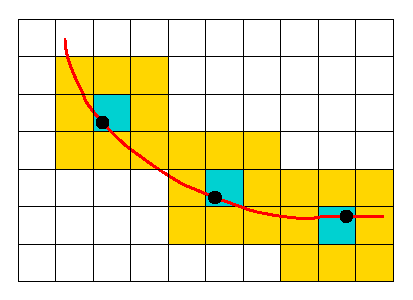
\includegraphics[width=0.4\linewidth]{images/selectA.eps} \qquad &
\qquad
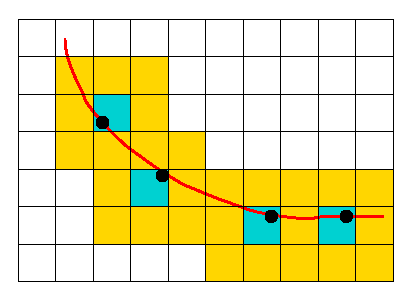
\includegraphics[width=0.4\linewidth]{images/selectB.eps} \\
(a) & (b)
\end{tabular}

\caption{2D illustration of vertex and cube selection.
(a) Selection which gives poor cover of the red curve.
The curve intersects an uncovered square.
(b) Selection which gives better cover of the red curve.
The curve is far away from any uncovered square.
}
\label{fig:select}
\end{figure}

\section{MergeSharp}

As show in Figure~\ref{alg:mergesharp}, Algorithm SHREC has three parts:
computation of isosurface vertex locations, 
selection of a well-spaced subset of vertices on sharp features
and merging of vertices around selected vertices.
Algorithm MergeSharp has a similar three parts,
but each part is substantially improved in SHREC.
We start with a brief description of MergeSharp
as presented in~\cite{bw-cisec-13}.

The computation of isosurface vertex locations
was described in Section~\ref{section:loc}.
The procedure in Section~\ref{section:loc}
returns not only a point $p_\cb$ on the isosurface,
but whether $p_\cb$ lies on a sharp corner, sharp edge or smooth portion 
of the isosurface.
Let $\Ccorner$ and $\Cedge$ be lists of cubes $\cb$ 
whose generated points $p_\cb$ lie on sharp corners and sharp edges, 
respectively.

As defined in Section~\ref{section:loc},
point $q_\cb$ is the centroid of interpolated intersection points
of the isosurface and grid edges of $\cb$.
Sort lists $\Ccorner$ and $\Cedge$ by increasing distance $|p_\cb - q_\cb|$
from $p_\cb$ to $q_\cb$.
Mark all the cubes as ``uncovered''.
Select the next uncovered cube $\cb$ in $\Ccorner$
where $p_\cb$ does not form a large angle triangle 
with vertices in previously selected cubes.
Merge $\cb$ with every uncovered vertex neighbor.
Mark all vertex neighbors of $\cb$ as covered.
The algorithm for $\Ccorner$ is shown in Figure~\ref{alg:select}.
After processing list $\Ccorner$, apply the same procedure to list $\Cedge$.

Note that the selection and merging are combined in the above description,
just as they are combined in~\cite{bw-cisec-13}.
In the modified version we present here,
those two steps will be separated.

There are problems with every one of the three steps of MergeSharp.
First, the vertex location $p_\cb$ generated by cube $\cb$
may lie outside $\cb$.
Moreover, point $p_\cb$ may lie outside of $\cb$
even if the sharp edge containing $p_\cb$ intersects $\cb$.
In addition, because of curvature, noise and numerical instability,
point $p_\cb$ could lie in some cube $\cb'$ adjacent to $\cb$
while point $p_{\cb'}$ lies inside $\cb$.
We will modify MergeSharp to generate point $p_\cb$ inside cube $\cb$
wherever possible.

Second, the selection step chooses cubes based on the proximity
of $p_\cb$ to $q_\cb$.
If a point $p_\cb$ is near $q_\cb$, 
it probably is located in cube $\cb$ 
and is a good approximation of the vertex location.
While this is reasonable,
it ignores the interaction between selected cubes.
MergeSharp does better when sharp edges are well-covered 
by the selected and covered cubes.
For instance, in the 2D illustration in Figure~\ref{fig:select}, 
the selected squares are packed together more closely
and their $3 \times 3$ regions do a better job of covering
the given curve.
We modified the MergeSharp selection to pack selected cubes 
more closely together.

Finally, the merging step merges cube $\cb$
with the the first selected cube adjacent to $\cb$.
Doing so sometimes distorts triangles, creating extremely thin triangles
and sometimes creating ``folds'' in the surface mesh.
We modify MergeSharp so that it prefers merging cubes which are facet
adjacent over merging edge adjacent or vertex adjacent cubes.
We add checks which avoid merging which creates small thin triangles
or creates folds.
We also extend the merging by one more cube in certain regions
to ensure good covering of sharp isosurface edges.


\begin{figure}[t]
\centering

\begin{tabular}{cc}
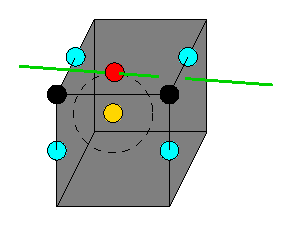
\includegraphics[width=0.4\linewidth]{images/centroid.eps} \qquad &
\qquad
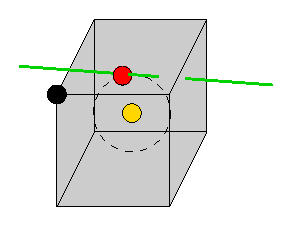
\includegraphics[width=0.4\linewidth]{images/center.eps} \\
(a) & (b)
\end{tabular}

\caption{The green line is the line containing the
sharp edge near cube $\cb$. 
Black cube vertices have scalar value above the isovalue.
(a) Green line intersects cube $\cb$
but point location $p^0_\cb$ (red) is outside cube $\cb$.
Cyan points are the intersection points of the isosurface
and the cube edges, computed using linear interpolation.
Gold point is $q_\cb$, the centroid of the cyan points, .
Red point is the closest point on the green line to $q_\cb$.
(b) Green line intersects cube $\cb$
but point location $p^1_\cb$ (red) is outside cube $\cb$.
Gold point is $\cb.\protect\Center$, the cube center.
Red point is the closest point on the green line to $\cb.\protect\Center$.
}
\label{fig:out_of_cube}
\end{figure}

\section{Generating Points on Sharp Features}
\label{section:generation}

\subsection{Computing Vertex Locations on Sharp Edges}

Consider an edge cube $\cb$.
By definition, edge cube $\cb$ is near some sharp edge.
The isosurface vertex $p_\cb$ associated with $\cb$ should lie
on that sharp edge.
However, that condition still gives one degree of freedom in selecting
the sharp point $p_\cb$.
One obvious additional condition is that if the sharp edge intersects $\cb$,
then $p_\cb$ should lie in $\cb$.
An additional condition is that if the sharp edge does not intersect $\cb$,
then $p_\cb$ should lie ``close to'' $\cb$ under some suitably defined metric.

Algorithm SHREC computes three different possible locations of $p_\cb$.
First, Algorithm SHREC computes $p^0_\cb$ 
by computing a line $L$ through the sharp edge and 
selecting the point on $L$ nearest the centroid point $q_\cb$.
Equation~\ref{eqn:Lindstrom}, for computing $p^0_\cb$ is given
in Section~\ref{section:loc}.
The idea is that the centroid point $q_\cb$ is a good approximation
for the intersection of $\cb$ and the isosurface,
and so one should choose a point near $q_\cb$.
If $p^0_\cb$ lies in $\cb$, then SHREC sets $p_\cb$ to $p^0_\cb$.

In most cases, if line $L$ intersects cube $\cb$.
then the point $p^0_\cb$ will lie in $\cb$.
However, if line $L$ is ``near'' some facet or edge of $\cb$,
then it is possible for $L$ to intersect $\cb$ but $p^0_\cb$ to lie
outside $\cb$.
(See Figure~\ref{fig:out_of_cube}(a).)

If $p^0_\cb$ lies outside $\cb$,
then let $p^1_\cb$ be the point on $L$ which lies closest 
to the center $\cb.\Center$ of cube $\cb$.
We can compute $p^1_\cb$ replacing $q_\cb$ by $\cb.\Center$
in Equation~\ref{eqn:Lindstrom}.
If $p^1_\cb$ is in $\cb$ while $p^0_\cb$ is not,
SHREC sets $p_\cb$ to $p^1_\cb$.

Unfortunately, it is possible that both $p^0_\cb$ and $p^1_\cb$ 
are not in $\cb$ even though $L$ intersects $\cb$.
(See Figure~\ref{fig:out_of_cube}(b).)
As a final step, we compute the point $p^2_\cb$ on $L$ which is closest 
to the center $\cb.\Center$ of $\cb$ under the $L_\infty$ metric.
If $L$ intersects $\cb$, then this point is guaranteed to lie in $\cb$.
Details for computing $p^2_\cb$ are in Appendix~\ref{appendix:Linf}.
If $p^2_\cb$ is in $\cb$ while $p^0_\cb$ and $p^1_\cb$ are not,
SHREC sets $p_\cb$ to $p^2_\cb$.

Instead of computing $p^0_\cb$, $p^1_\cb$ and $p^2_\cb$, 
we could compute and use only $p^2_\cb$.
However, the computations of $p^0_\cb$ and $p^1_\cb$ are much faster,
and their locations are preferable to $p^2_\cb$ when they are
contained in cube $\cb$.
Algorithm MergeSharp computes only $p^0_\cb$.

\begin{figure}[t]
\centering

\begin{tabular}{cc}
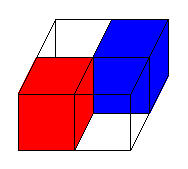
\includegraphics[width=0.4\linewidth]{images/shared_edge.eps} \qquad &
\qquad

\includegraphics[width=0.4\linewidth]{images/shared_edge_B.eps} \\
(a) & (b)
\end{tabular}

\caption{(a) Two grids cubes sharing an edge $\eb$.
(b) The two other cubes (gold) which also contain $\eb$.
}
\label{fig:shared_edge}
\end{figure}

\begin{figure}[t]
\centering

\begin{tabular}{cc}
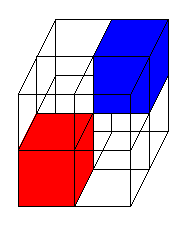
\includegraphics[width=0.4\linewidth]{images/shared_vertex.eps} \qquad &
\qquad
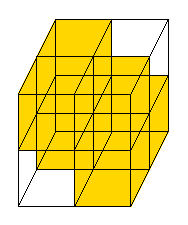
\includegraphics[width=0.4\linewidth]{images/shared_vertex_B.eps} \\
(a) & (b)
\end{tabular}

\caption{(a) Two grids cubes sharing a vertex $v$.
(b) The six other cubes (gold) which also contain $v$.
}
\label{fig:shared_vertex}
\end{figure}

\subsection{Swapping Locations}

Many of the problems in Algorithm SHREC (and MergeSharp) occur when
isosurface vertex location $p_\cb$ lies outside of cube $\cb$.
Thus, it is always preferable that $p_\cb$ be in $\cb$.
This is not always possible since the sharp edge or corner near $\cb$
may not intersect $\cb$.
However, in cases where a sharp edge or corner intersects $\cb$,
we would like $p_\cb$ to be in $\cb$.

The computation of a sharp edge or corner near $\cb$ depends
upon gradients in the neighborhood of $\cb$.
The set of such gradients changes for each cube $\cb$.
Because of the inaccuracy in computing sharp edges and corners,
it is possible that $p_\cb$ lies in a cube $\cb'$ adjacent to $\cb$
while $p_{\cb'}$ is not contained in $\cb$.
In some cases,
point $p_\cb$ lies in $p_{\cb'}$ while $p_{\cb'}$ lies in $p_{\cb}$.
In those cases,
we simply swap $p_\cb$ and $p_{\cb'}$.
In other cases, point $p_{\cb'}$ lies in some third cube $\cb''$.
In that case, we simply set $p_{\cb'}$ to $p_\cb$.

The setting of isosurface vertex locations from adjacent cubes
increases the number of cubes $\cb$ containing 
their associated vertext locations $p_\cb$.
Note that if the initial location $p_\cb$ lies in $\cb$,
then we never change $p_\cb$.


\begin{figure}
\centering
\begin{tabular}{cc}
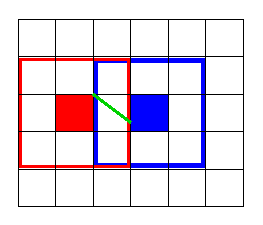
\includegraphics[width=1.2in]{images/config2D_2_0.eps} \qquad &
\qquad
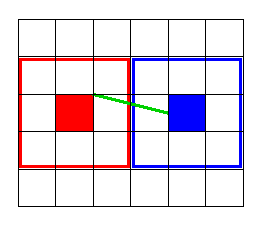
\includegraphics[width=1.2in]{images/config2D_3_0.eps} \\
(a) Configuration (2,0). & (b) Configuration (3,0). \\
\\
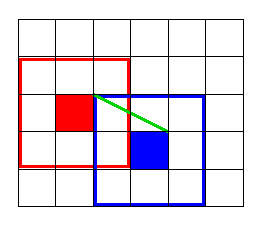
\includegraphics[width=1.2in]{images/config2D_2_1.eps}
\qquad &
\qquad
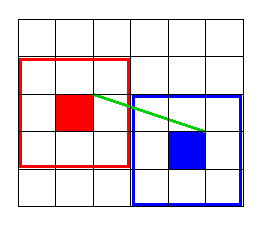
\includegraphics[width=1.2in]{images/config2D_3_1.eps} \\
(c) Configuration (2,1). & (d) Configuration (3,1).
\end{tabular}
\caption{Tightly packed 2D configurations of selected squares.
Selected squares and $3 \times 3$ region around each square.
Line segments with endpoints on the two selected squares 
(e.g., the green line segments) are contained
within the union of the two $3 \times 3$ regions.}
\label{fig:packed2D}
\end{figure}

\begin{figure}[t]
\centering
\begin{tabular}{cc}
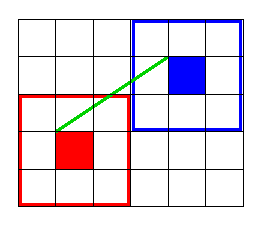
\includegraphics[width=1.2in]{images/config2D_3_2.eps} \qquad &
\qquad
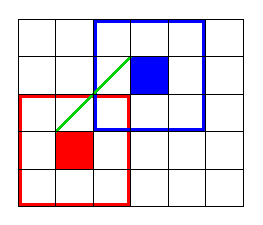
\includegraphics[width=1.2in]{images/config2D_2_2.eps} \\
(a) Configuration (3,2). & (b) Configuration (2,2). 
\end{tabular}
\caption{Problematic 2D configurations of selected squares.
Selected squares and $3 \times 3$ region around each square.
(a) The green line segment is not contained within the union
of the two $3 \times 3$ regions.
(b)~The green line segment intersects the boundary
of the union of the two $3 \times 3$ regions.}
\label{fig:loose2D}
\end{figure}

\begin{figure}[t]
\centering
\begin{tabular}{cc}
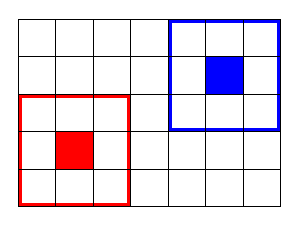
\includegraphics[width=1.2in]{images/config2D_4_2.eps} \qquad &
\qquad
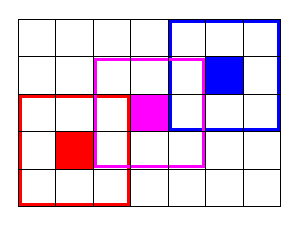
\includegraphics[width=1.2in]{images/config2D_4_2_B.eps} \\
(a) Configuration (4,2). & (b) Additional cube.
\end{tabular}
\caption{(a) Configuration (4,2) has space between the $3 \times 3$
regions around each selected square.
(b) Additional cube (magenta) which packs tightly with two other squares.}
\label{fig:config2D_4_2}
\end{figure}

\begin{figure*}
\centering
\begin{tabular}{cccc}
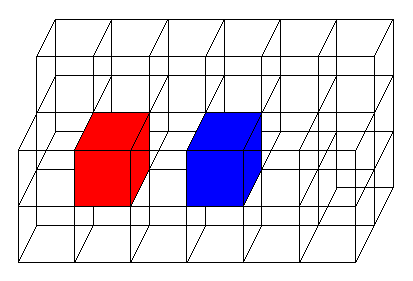
\includegraphics[width=1.2in]{images/config3D_2_0_0.eps} \qquad &
\qquad
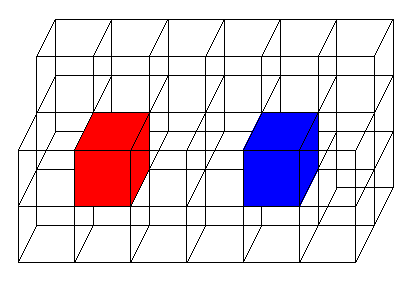
\includegraphics[width=1.2in]{images/config3D_3_0_0.eps}
\qquad &
\qquad
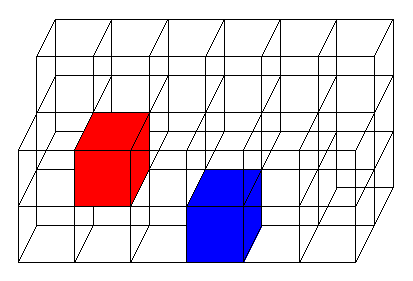
\includegraphics[width=1.2in]{images/config3D_2_1_0.eps}
\qquad &
\qquad
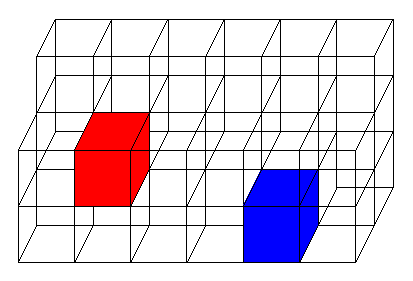
\includegraphics[width=1.2in]{images/config3D_3_1_0.eps} \\
(a) Configuration (2,0,0). & (b) Configuration (3,0,0). 
  & (c) Configuration (2,1,0). & (d) Configuration (3,1,0).
\end{tabular}
\caption{Tightly packed 3D configurations of selected cubes.}
\label{fig:packed3D}
\end{figure*}

\begin{figure*}
\centering
\begin{tabular}{ccc}
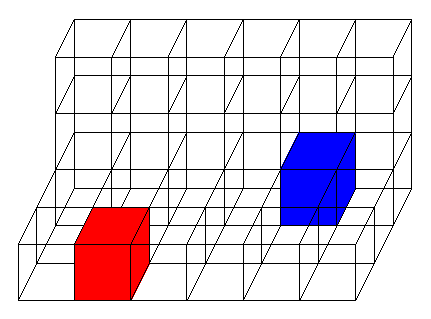
\includegraphics[width=1.2in]{images/config3D_3_2_0.eps} \qquad &
\qquad
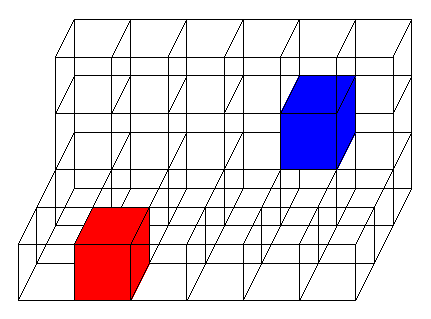
\includegraphics[width=1.2in]{images/config3D_3_2_1.eps}
\qquad &
\qquad
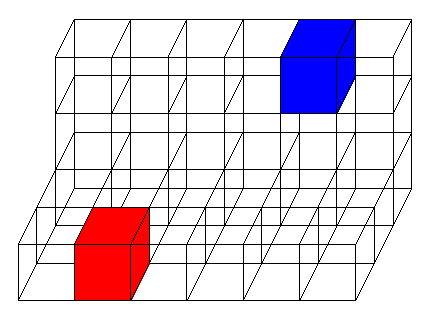
\includegraphics[width=1.2in]{images/config3D_3_2_2.eps} \\
(a) Configuration (3,2,0). & (b) Configuration (3,2,1). 
  & (c) Configuration (3,2,2).
\end{tabular}
\caption{Problematic 3D configurations of selected cubes.}
\label{fig:loose3D}
\end{figure*}

\begin{figure}[t]
\centering

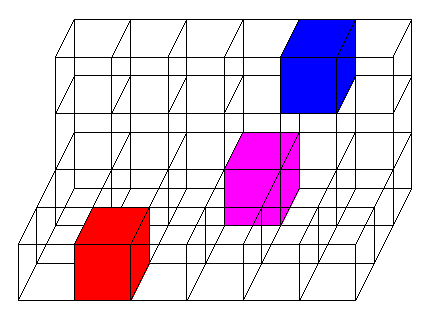
\includegraphics[width=1.2in]{images/config3D_3_2_2_B.eps}

\caption{Problematic interaction of red and blue cubes
in configuration (3,2,2) is blocked by magenta cube.}
\label{fig:blocked3D}
\end{figure}

\subsection{Locations on Planes}

Consider two grid cubes, $\cb$ and $\cb'$, 
which intersect in an edge $\eb$ but not in any facet.
(See Figure~\ref{fig:shared_edge}.)
Two other grid cubes, $\tcb$ and $\tcb'$ share edge $\eb$.
A sharp edge which passes through $\cb$ and $\cb'$ must intersect
either $\tcb$ or $\tcb'$.
(In the exceptional case, the edge passes through $\eb$,
in which case it intersects both $\tcb$ and $\tcb'$.)
Since the edge intersects either $\tcb$ and $\tcb'$,
either $p_\tcb$ should lie in $\tcb$ 
or $p_{\tcb'}$ should lie in $\tcb'$.
However, because of inaccuracies in computing sharp edges and corners,
neither condition may hold.

To ensure that either $p_\tcb$ lies in $\tcb$
or $p_{\tcb'}$ lies in $\tcb'$,
Algorithm SHREC computes the plane $\pi$ containing $\eb$
and perpendicular to the line from $\cb.\Center$ to $\cb'.\Center$.
SHREC then computes the intersection of the line $L$ containing $\eb$
and plane $\pi$.
This intersections point, $p_I$, lies in either $\tcb$ or $\tcb'$.
If $p_I$ lies in $\tcb$ and $p_\tcb$ is not in $\tcb$,
SHREC sets $p_\tcb$ to $p_I$.
If $p_I$ lies in $\tcb'$ and $p_{\tcb'}$ is not in $\tcb'$,
SHREC sets $p_{\tcb'}$ to $p_I$.

Next consider the case of two grid cubes, $\cb$ and $\cb'$, 
which intersect in a vertex $v$ but not in any edge.
(See Figure~\ref{fig:shared_vertex}.)
Six other grid cubes share vertex $v$ with $\cb$ and $\cb'$.
A sharp edge which passes through $\cb$ and $\cb'$ must intersect
one of these six other grid cubes.
(In the exceptional case, the edge passes through $v$,
in which case all six.)
Since the edge intersects one of the six grid cubes,
point $p_{\tcb}$ should lie in $\tcb$ for one of the six grid cubes $\tcb$.
Again because of inaccuracies in computing sharp edges and corners,
point $p_{\tcb}$ may not be in $\tcb$ for any of the six grid cubes $\tcb$.

To ensure that $p_\tcb$ lies in $\tcb$ for one of the six grid cubes,
Algorithm SHREC computes the plane $\pi$ containing $v$
and perpendicular to the line from $\cb.\Center$ to $\cb'.\Center$.
SHREC then computes the intersection of the line $L$ containing $\eb$
and plane $\pi$.
This intersections point, $p_I$, lies in at least one of the six grid cubes.
If $p_I$ lies in cube $\tcb$ and $p_\tcb$ is not in $\tcb$,
SHREC sets $p_\tcb$ to $p_I$.

The computation in this section ensures ``continuity'' in the cubes
which intersect a sharp edge.
If a sharp edge intersects a cube $\cb$,
then the edge should intersect two cubes $\cb'$ and $\cb''$
which share a facet with $\cb$.
SHREC's computation of edge-plane intersections described above,
ensures that if $\cb'$ and $\cb''$ are active cubes,
then $\cb'$ will contain $p_{\cb'}$ and $\cb''$ will contain $p_{\cb''}$.

\section{Selecting Points on Sharp Features}
\label{section:selection}

Algorithm SHREC selects a well-spaced subset of the edge and corner cubes
and merges isosurface vertices adjacent cubes 
with the vertices generated by the selected cubes.
To ensure that the isosurface vertices on sharp features are well-spaced,
SHREC never selects two cubes which have a common vertex.
Whenever SHREC selects a cube $\cb$,
any adjacent cube sharing a vertex with $\cb$ is marked as ``covered''
by $\cb$.
SHREC never selects a covered cube.

As noted in Section~???, 
SHREC does better when selected cubes 
are packed ``tightly'' together.
In particular, SHREC tries to avoid certain configurations of nearby cubes.

Consider cubes $\cb$ and $\cb'$ with grid indices $(x_0,x_1,x_2)$
and $(x'_0,x'_1,x'_2)$, respectively.
(A cube with grid indices $(x_0,x_1,x_2)$ is in column $x_0$, row $x_1$
and $z$-plane $x_2$ of the grid.)
The {\em distance vector} between the cubes is
$(|x_0-x'_0|, |x_1-x'_1|, |x_2-x'_2|)$.
Two grid cubes are in configuration $(a_0,a_1,a_2)$ if the distance vector
between the cubes is some permutation of $(a_0,a_1,a_2)$.
Figures~\ref{fig:packed2D}, \ref{fig:loose2D}, \ref{fig:config2D_4_2}
and~\ref{fig:packed3D},
contain examples of 2D and 3D configurations of grid cubes.

We can get some insight into 3D configurations of grid cubes
by considering the 2D configurations of grid squares.
Figure~\ref{fig:packed2D} contains configurations $(2,0)$, $(3,0)$,
$(2,1)$ and $(3,1)$ of grid squares.
The $3 \times 3$ regions around the selected squares are ``tightly packed''
so that any line segment with endpoints in the selected squares
is contained within the union of the two $3 \times 3$ regions.

Figure~\ref{fig:loose2D} contains configurations $(3,2)$ and $(2,2)$
of grid squares.
With configuration $(3,2)$, some line segments with endpoints
in the selected squares are not contained within the union
of the $3 \times 3$ regions.
Configuration $(2,2)$ is somewhat better,
since all line segments with endpoints in the selected squares
are contained within the union of the $3 \times 3$ regions.
Unfortunately, they are only barely contained.
The green line segment in Figure~\ref{fig:loose2D}(b) intersects
the boundary of the $3 \times 3$ region.
Slightly curving the segment could mean that it no longer was contained
in the union.

Note that if selected squares are suitably far apart,
then additional squares can be selected between them.
For instance, a magenta square can be selected between the two colored squares
in Figure~\ref{fig:config2D_4_2}(a) and the $3 \times 3$ regions
will fit together tightly.

Some examples of tightly packed 3D configurations of cubes are given
in Figure~\ref{fig:packed3D}.
Any line segment with endpoints in the two selected cubes
will be well contained within the $3 \times 3 \times 3$ region 
around each selected cube.

Figure~\ref{fig:loose3D} contains three problematic configurations,
$(3,2,0)$, $(3,2,1)$ and $(3,2,2)$,
of  selected cubes.
Line segments with endpoints in the two selected cubes
may lie outside the $3 \times 3 \times 3$ region around each selected cube.
SHREC attempts to avoid selecting cubes with these configurations.

If two selected cubes, $\cb$ and $\cb'$, 
are in configuration $(2,2,0)$, $(2,2,1)$ or $(2,2,2)$,
then a line segment with endpoints in $\cb$ and $\cb'$
could intersect the boundary of the union of the $3 \times 3 \times 3$
regions around $\cb$ and $\cb'$.
Such configurations are undesirable.
Unfortunately, we found that avoiding such configurations is too restrictive.

Consider two cubes, $\cb$ and $\cb''$ 
in a $(3,2,0)$, $(3,2,1)$ or $(3,2,2)$ configuration.
If a third selected cube $\cb'$ lies between $\cb$ and $\cb''$,
then the sharp edge will pass from $\cb$ to $\cb'$ to $\cb''$.
The selection of $\cb'$ ``blocks'' the problematic interaction 
of $\cb$ and $\cb''$.
If cubes $\cb$ and $\cb'$ are selected,
then SHREC will permit the selection of $\cb''$,
even though $\cb$ and $\cb''$ have a configuration $(3,2,*)$.
Figure~\ref{fig:blocked3D} contains an example of two cubes 
in a $(3,2,2)$ configuration and a third cube between them.

More formally,
let $\cb$, $\cb'$ and $\cb''$ be grid cubes with grid indices
$(x_0,x_1,x_2)$, $(x'_0,x'_1,x'_2)$ and $(x''_0,x''_1,x''_2)$, respectively.
Cube $\cb'$ {\em separates} $\cb$ from $\cb''$
if $x'_i \in [x_i,x''_i]$ for $i = 0,1,2$
and $x_i < x'_i < x''_i$ or $x_i > x'_i > x''_i$ for some $i$.
SHREC avoids selecting cube $\cb''$ if some already selected cube $\cb$
forms a $(3,2,0)$ or $(3,2,1)$ or $(3,2,2)$ configuration with $\cb''$
and no already selected cube separates $\cb$ from $\cb''$.

SHREC first selects corner cubes.
When the corner location is inside an active cube,
SHREC selects the active cube containing the corner.
When the corner location is not in an active cube,
SHREC selects the active cube ``closest'' to the corner location
by choosing the cube whose center has minimum $L_\infty$ distance
to the corner.

SHREC next selects edge cubes which are ``near'' the corner cubes,
i.e., they are contained in an $7 \times 7 \times 7$ region
around each corner cube.
Selecting edge cubes near corners poses special challenges
since there are multiple sharp edges ending at a corner.
Selecting a cube which is near two such sharp edges
can obscure one of the edges.

Let $\cb$ be a corner cube and let $\cb'$ be an edge cube
which is in a $(2,0,0)$, $(2,1,0)$ or $(2,1,1)$ configuration with $\cb$.
Let $\cb''$ be any cube sharing an edge or facet with $\cb'$
which is contained in the $5 \times 5 \times 5$ region
but is not covered by $\cb$.
If $\cb''$ is active and an edge cube,
then SHREC attempts to avoid selecting cube $\cb'$.

Once edge cubes near corners are selected,
SHREC could iterate by selecting uncovered edge cubes 
near already selected cubes.
If no uncovered edge cubes were near selected cubes,
SHREC could select an arbitrary uncovered edge cube
and extend the set of selected cubes from that cube.
By not selecting a cube $\cb''$ 
if it forms a $(3,2,0)$, $(3,2,1)$ or $(3,2,2)$
with an already selected cube $\cb$ 
(and is not separated by a selected cube from $\cb$,)
SHREC would produce a tight packing of selected cubes.

The algorithm outlined in the previous paragraph would produce
a good set of selected cubes but it is highly sequential.
One of the best aspects of the Marching Cubes and dual contouring algorithms
is their local, distributed, paralellizable nature.
Sequentially extending the set of selected cubes would totally destroy
that aspect of the algorithms.
Instead of selecting cubes using the sequential algorithm given above,
SHREC divides the regular grid 
into overlapping $6 \times 6 \times 6$ regions,
selects cubes from the boundaries of those regions and then from their interior.
The algorithm is completely local and easily distributed and parallelizable.

Each grid cube has an index $(x_0, x_1, x_2)$.
SHREC processes the grid cubes by reducing the indices modulo six
to $(x_0 \bmod 6, x_1 \bmod 6, x_2 \bmod 6)$.
SHREC first selects edge cubes with indices congruent to $(0,0,0)$ modulo six.
SHREC next selects edge cubes with indices congruent modulo six
to $(\pm 1,0,0)$ or $(0, \pm 1, 0)$ $(0, 0, \pm 1)$.
SHREC then selects edge cubes with indices congruent modulo six
to $(\pm 2,0,0)$ or $(0, \pm 2, 0)$ $(0, 0, \pm 2)$.
Finally, SHREC selects edge cubes with indices congruent modulo six
to $(3,0,0)$ or $(0, 3, 0)$ $(0, 0, 3)$.
SHREC does not select an edge cube $\cb$ if some already selected cube $\cb'$
forms configuration $(3,2,0)$, $(3,2,1)$ or $(3,2,2)$ with $\cb$
and no already selected cube separates $\cb$ from $\cb''$.

SHREC next selects edge cubes which are some permutation
of $(k_a,k_b,0)$ modulo six,
starting first with permutations of $(\pm 1, \pm 1, 0)$
and ending with permutations of $(3, 3, 0)$.
Finally, SHREC selects edge cubes which are permutations
$(k_a, k_b, k_c)$ modulo six,
starting first with permutations of $(\pm 1, \pm 1, \pm 1)$
and ending with $(3, 3, 3)$.

It is possible that the selection of two edge cubes $\cb$ and $\cb''$
at distance five apart can force the selection of an edge cube $\cb'$
which has a $(3,2,1)$ or $(3,2,2)$ configuration 
with either $\cb$ or $\cb''$.
This happens if the distance vector between $\cb$ and $\cb''$
is $(5,3,2)$.
Thus, in addition to avoiding $(3,2,*)$ configurations,
SHREC also avoids selecting two cubes, $\cb$ and $\cb''$, 
which form a $(5,3,2)$ configuration.
Of course, if $\cb$ and $\cb''$ are separated by some other selected cube,
then they can both be selected.

While the above rules select a set of cubes which almost completely cover
the sharp edges of a surface,
it is possible that the configuration restrictions leave a few areas uncovered.
Therefore, SHREC repeats the selection process to select any remaining
uncovered edge cubes but drops the configuration restrictions.


\section{Merging Points with Features Points}
\label{section:merging}

\section{Parameters}
\label{section:parameters}



\section{Measuring Angular Distance between Surfaces}
\label{section:angular_distance}

As described in Section~\ref{section:related},
we evaluated MergeSharp in~\cite{bw-cisec-13}
by extracting sharp mesh edges (dihedral angle less than $140^\circ$)
and comparing the 1-skeleton formed
by those sharp edges with the 1-skeleton of the sharp edges 
in an ideal surface.
We present here a different way of evaluating 
a reconstructed mesh containing sharp features.










\newcommand{\fCII} {\emath{f^{C \times 2}}}
\newcommand{\fPII} {\emath{f^{P \times 2}}}
\section{Experimental Results on Synthetic Data}\label{sec:synData}
\subsection{Synthetic Scalar and Gradient Data}
\label{section:synthetic}

To measure the quality of our reconstruction,
we used a number of synthetic scalar and gradient data sets.
Given a point $p$,
let $f^{L_1}_{p}(q)$ be the $L_1$ distance from $p$ to $q$.
A Cube data set is generated by sampling $f^{L_1}_p$
and its gradients on vertices of the regular grid.

Level sets of $f^{L_1}_p$ are cubes whose edges are
parallel to the coordinate axes
and whose facets are orthogonal to those axes.
By rotating $f^{L_1}_p$ around $p$, 
we can generate a scalar field whose level sets are cubes
that are not axis-aligned.
By taking the minimum of two (rotated) scalar fields, 
$f^{L_1}_p$ and $f^{L_1}_{p'}$, 
centered around two different points, $p$ and $p$', respectively,
we get a scalar field whose level sets are the boundaries
of the unions of the two cubes.
We call such data sets TwoCubes and use them 
with various rotations as test sets.

Let $\ell$ be a line.
Let $f^C_{\ell}(q)$ be the Euclidean distance from point $q$ to $\ell$.
The level sets of $f^C_{\ell}(q)$ are infinite cylinders around $\ell$.
Let $\fCII_{\ell,r}(q)$ equal $|f^C_{\ell}(q) - r|$.
The level sets of $\fCII_{\ell,r}(q)$  are pairs of infinite cylinders
at equal distances from the cylinder of radius $r$ around $\ell$.
Let $\fPII_{p,\ell}(q)$ be the distance from $q$ to the plane 
that contains point $p$ and is orthogonal to $\ell$.
Let $f^A_{p,\ell,r}(q)$ be the maximum 
of $\fCII_{\ell,r}(q)$ and of $\fPII_{p,\ell}(q)$.
The level sets are the boundaries of thickened annuli.

The width of the thickened annuli defined by $f^A_{p,\ell,r}$
equals their height.
We can adjust change the difference between the width and height
by adding a constant $c$ to $\fCII_{\ell,r}$.
Let $f^A_{p,\ell,r,c}(q)$ be the maximum 
of $\fCII_{\ell,r}(q)+c$ and of $\fPII_{p,\ell}(q)$.
If $c$ is positive, then the height is $c$ units greater than the width.
If $c$ is negative, then the height is $c$ units less than the width.

Define $f^F_{p,\ell,r,c}(q)$ as the minimum
of $f^A_{p,\ell,r,c}(q)$ and $f^A_{p,\ell,r,-c}(q)$.
The level sets of $f^F_{p,\ell,r,c}(q)$ are the boundaries
of the unions of two thickened annuli.
One annuli has height $c$ units greater than its width
while the other has height $c$ units less than its width.
A Flange data set is a regular grid sampling of $f^F_{p,\ell,r,c}(q)$. 
We use the Flange data sets as test sets.

\subsection{Isosurface Reconstruction on Synthetic Data}
We ran SHREC on 40 Flange datasets with different orientations. Figure~\ref{fig:flangeAngle} shows the summary results.
With synthetic gradients, SHREC produced ``NO" degree errors on the 40 test cases.
Figure~\protect\subref*{fig:flangeAngle3} shows the number of CountDegree errors in running SHREC with gradients computed from the scalar volume using RELIGRAD.
Fourteen cases ($35\%$) produced no degree errors. The mean error was 4.5. The maximum error was 22.
Figure~\protect\subref*{fig:flangeAngle1} shows the number of simplices with angle difference greater than 30$^\circ$, 40$^\circ$ and 50$^\circ$ from the original mesh for the 40 test cases. Figure~\protect\subref*{fig:flangeAngle2} shows  the number of simplices versus the angle difference for one particular dataset (id 16). This particular dataset has no CountDegree errors, it has three simplices with surface angle difference greater than 30 degrees from the original and one simplex above 40 degrees. The mesh itself has approximately 133 thousand simplices. 
Figure~\ref{fig:flange1} shows the result on a single dataset. The magnified region shows edges with dihedral angle less than $140^\circ$ in red blended with a subset of the ``non-sharp" edges. 
\begin{figure}[tb]
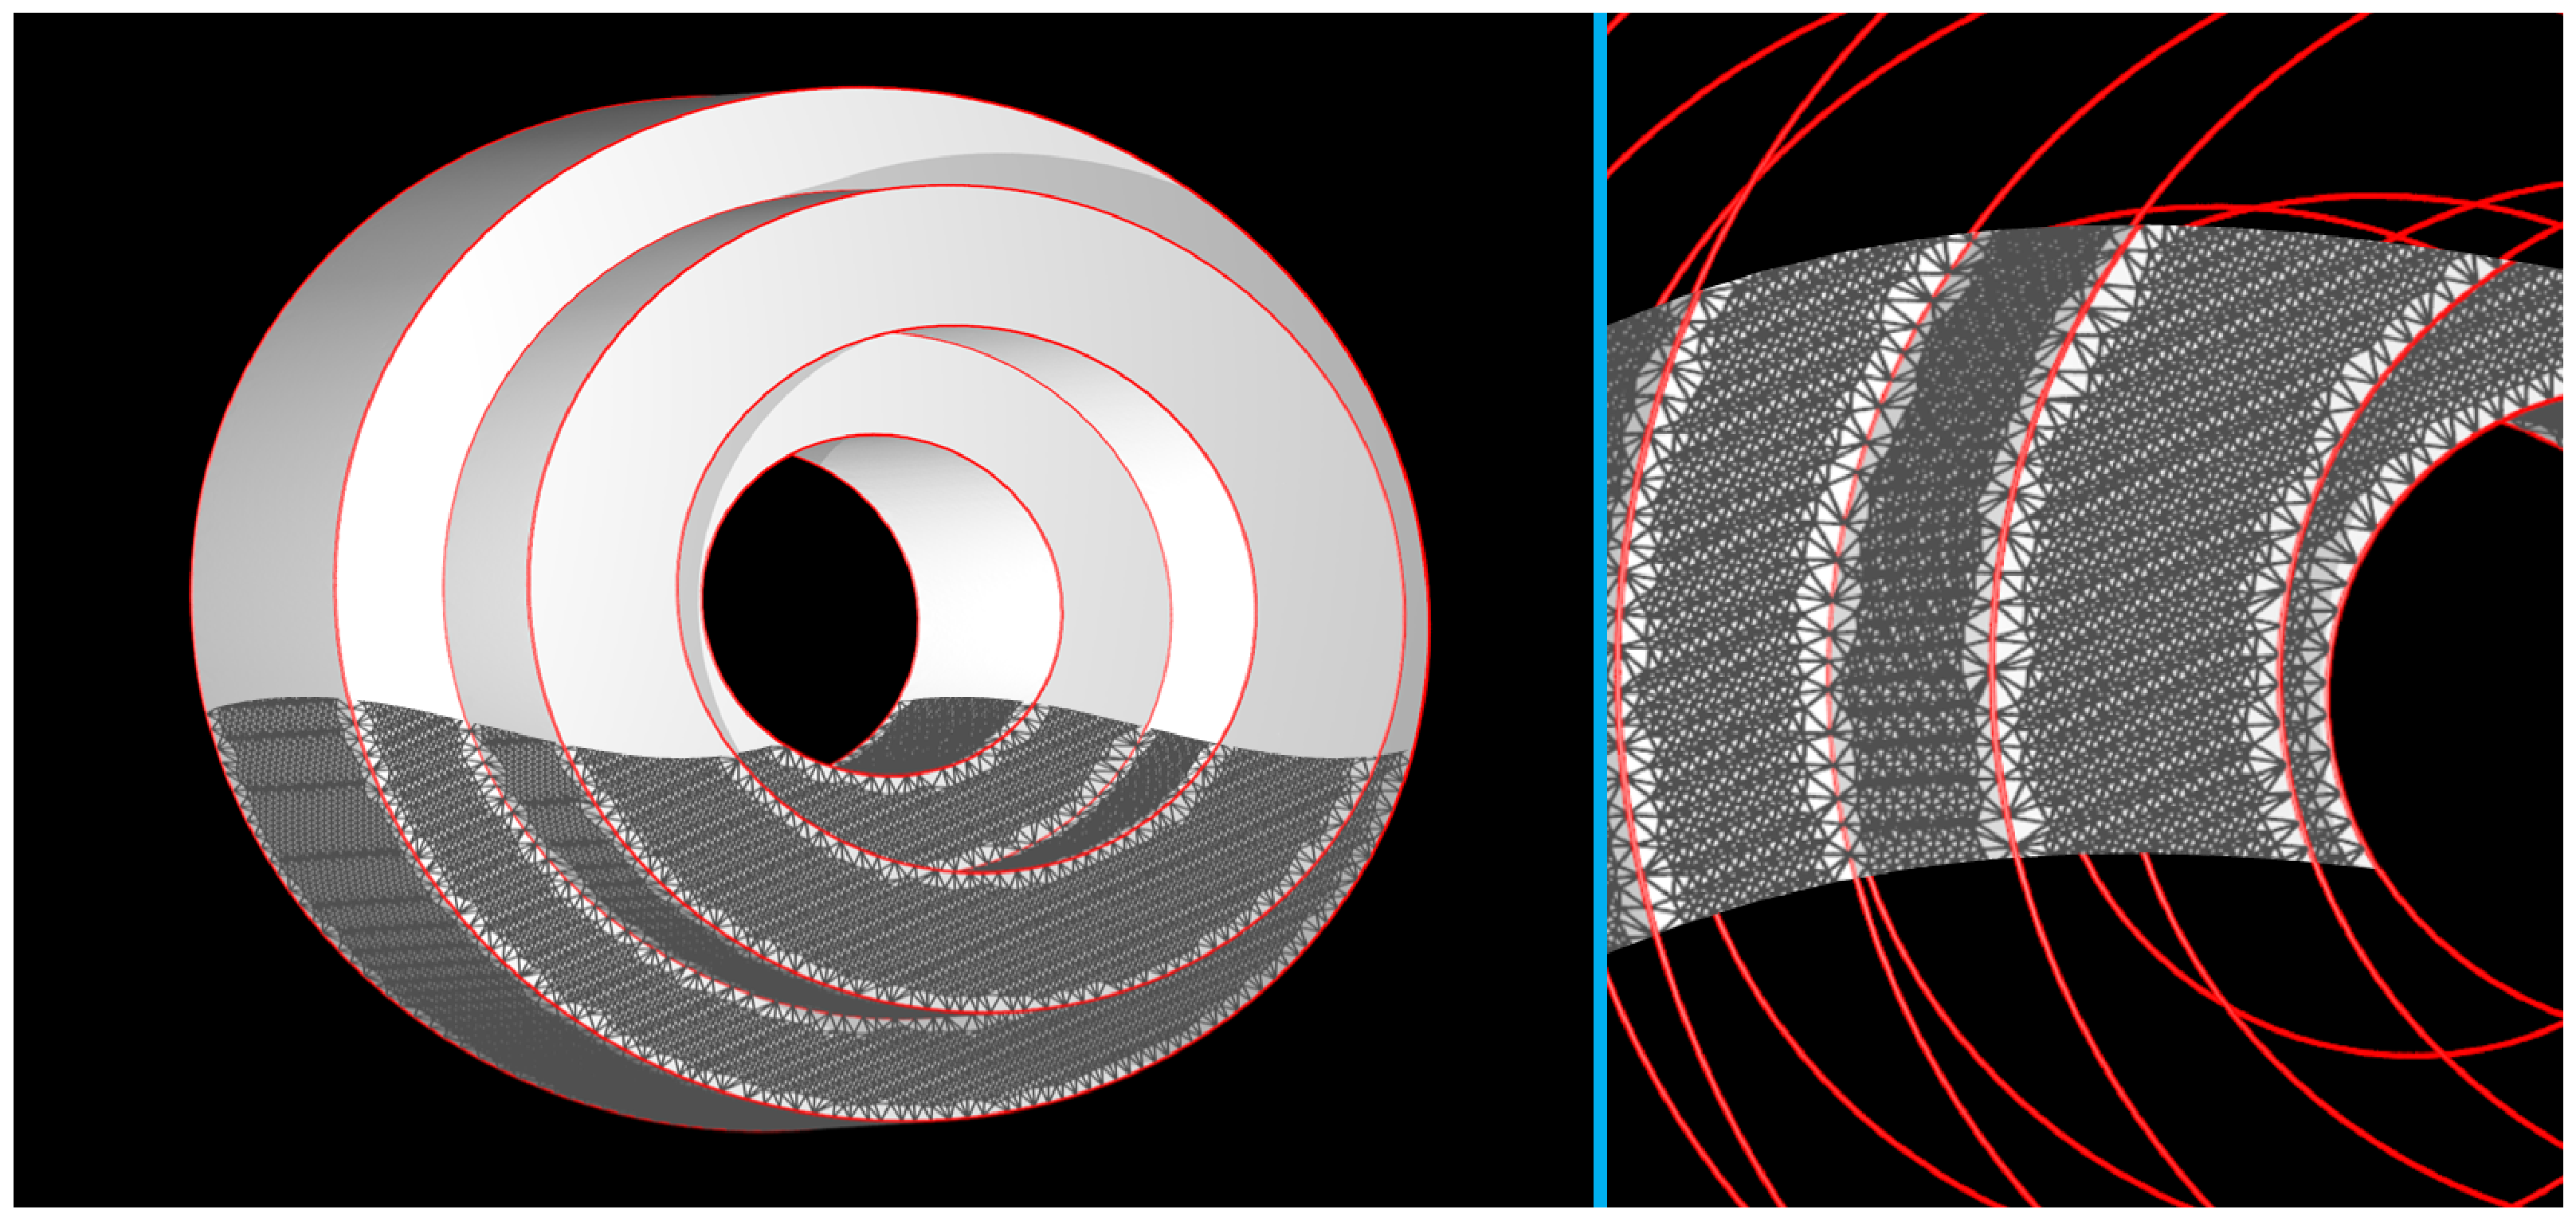
\includegraphics[width=\linewidth]{images/shrecFlangeCombine2.eps}
\caption{Result of SHREC on a Flange dataset. ``Sharp" edges (with dihedral angle less than $140^\circ$) are marked in red. 
``Smooth" edges are in dark grey. The magnified region shows a blend of the ``sharp" edges with a subset of the ``smooth" edges.}
\label{fig:flange1}
\end{figure}
\begin{figure*}[tb]
	\subfloat[]{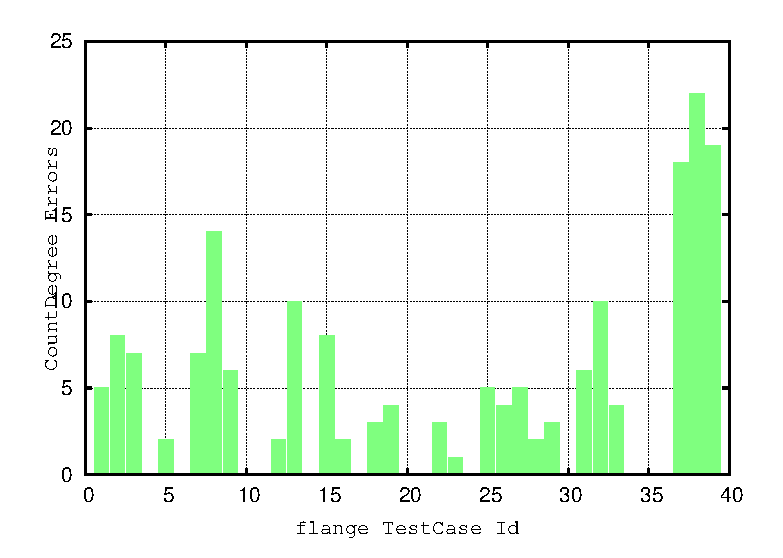
\includegraphics[width=0.33\linewidth]{images/flangeAngle3.eps}\label{fig:flangeAngle3}}
	\subfloat[]{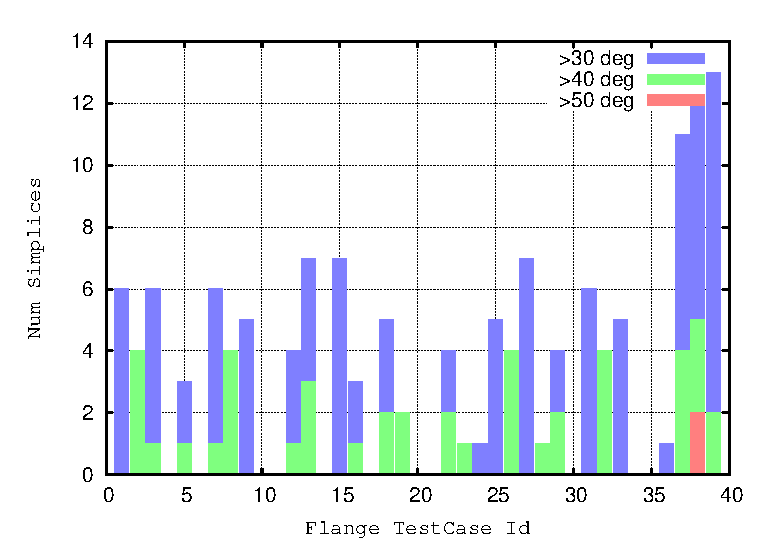
\includegraphics[width=0.33\linewidth]{images/flangeAngle1.eps}\label{fig:flangeAngle1}}
	\subfloat[]{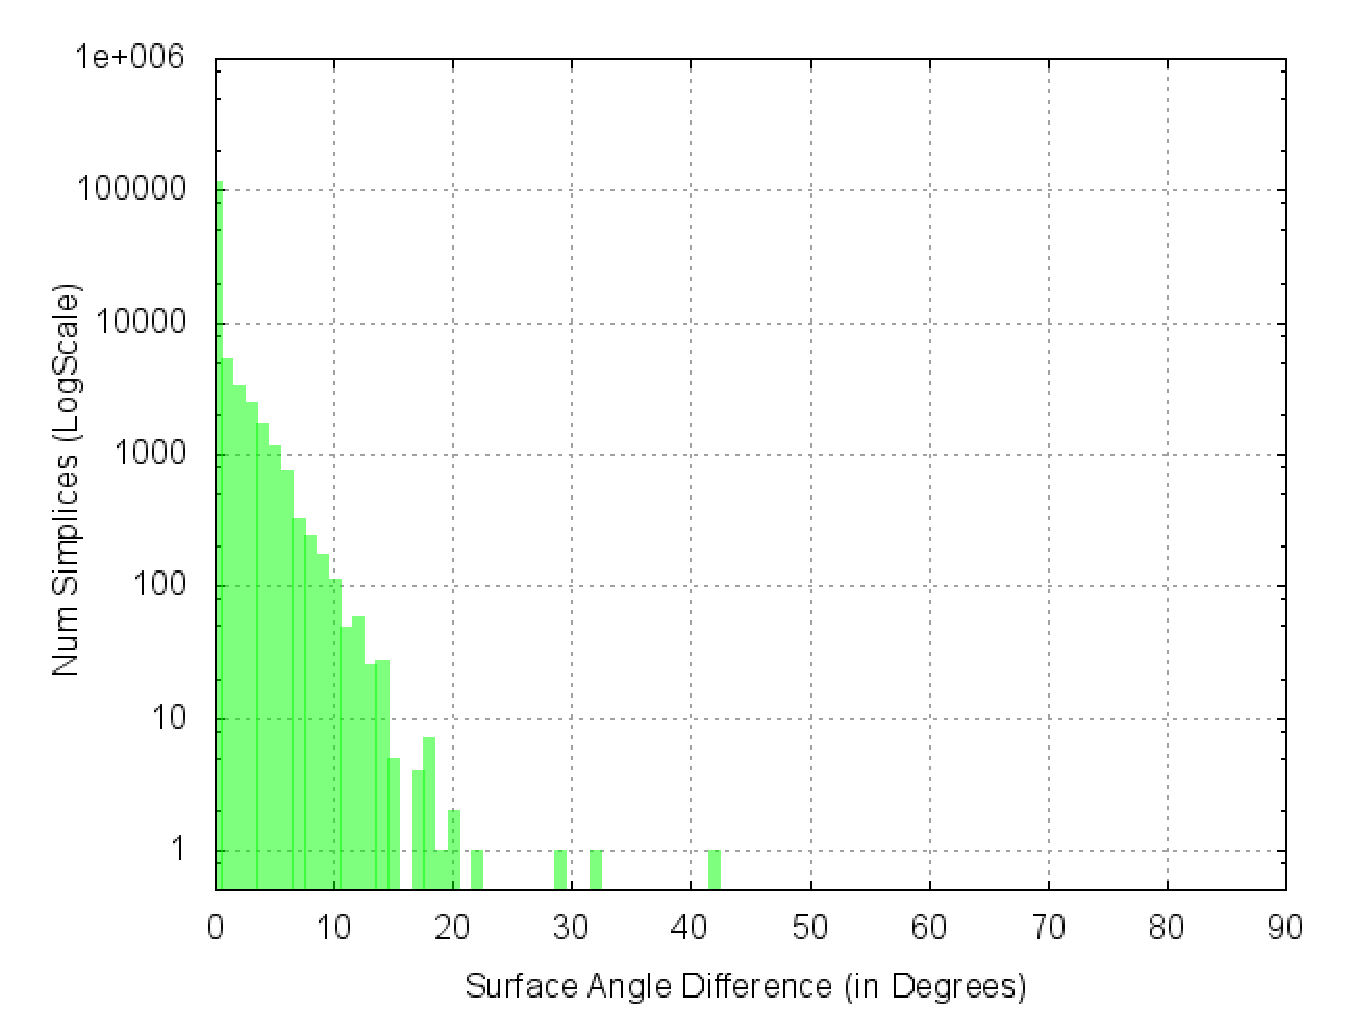
\includegraphics[width=0.33\linewidth]{images/flangeAngle2.eps}\label{fig:flangeAngle2}}
	\caption{SHREC with gradients computed from scalar data using RELIGRAD on 40 datasets. (a) Number of CountDegree errors. (b) Number of simplices with angle difference to ``perfect" mesh above 30, 40 and 50 degrees. (b) Shows the angle distribution of one particular case (16) which has three simplices over 30 degrees and 1 above 40 degrees. Total number of simplices is ~133k.}\label{fig:flangeAngle}
\end{figure*}
\begin{figure*}[tb] 
	\centering
	\subfloat[]{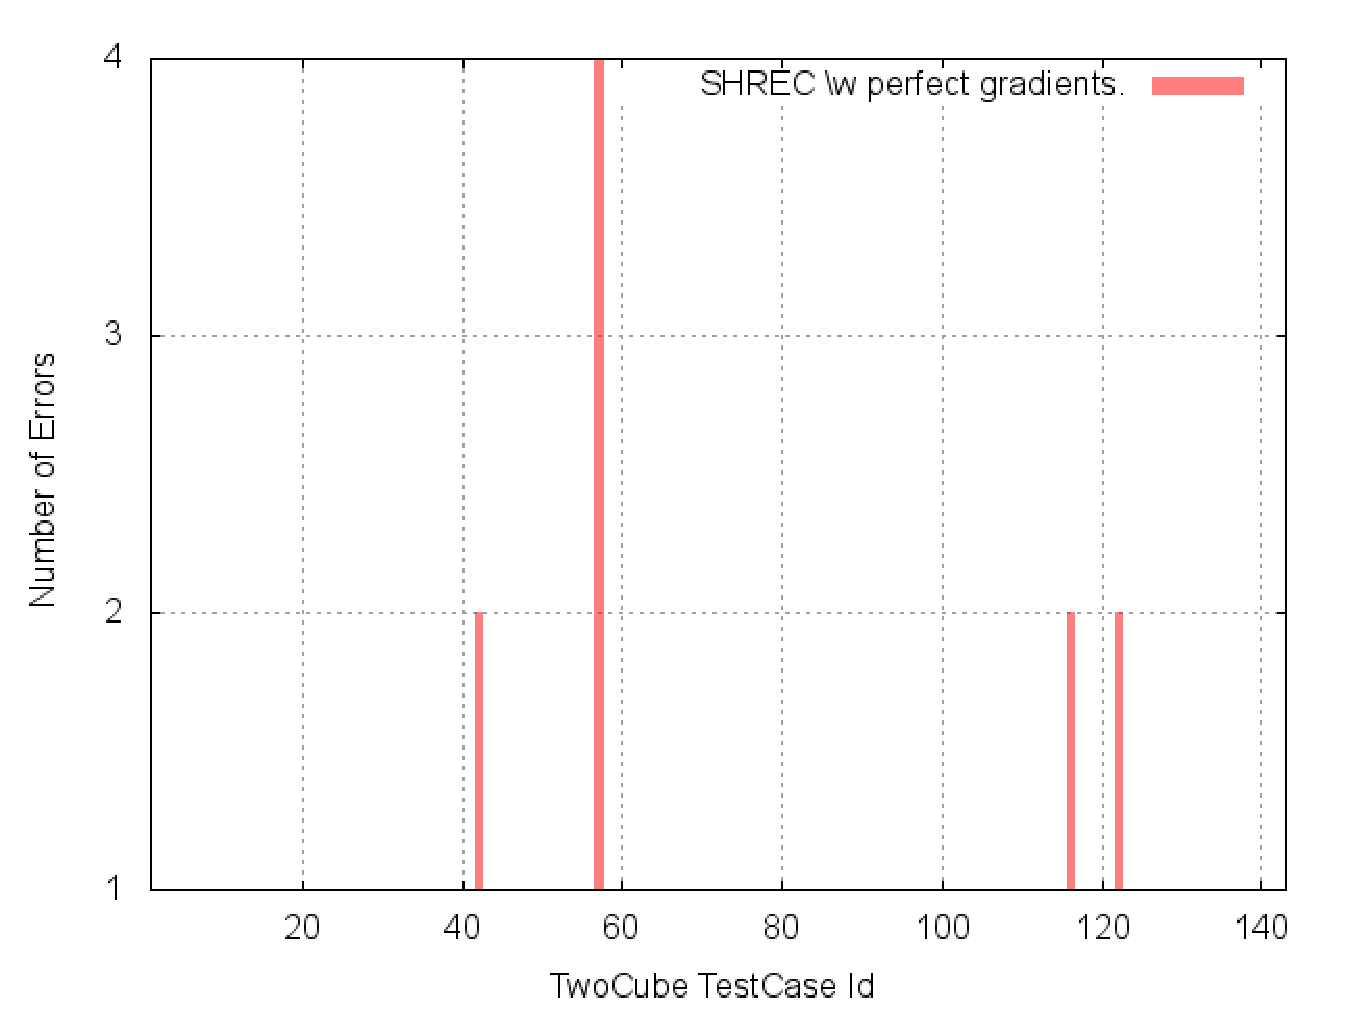
\includegraphics[width=0.3\linewidth]{images/shrecResCol1.eps}\label{fig:shrecTwoCube:a}}
	\subfloat[]{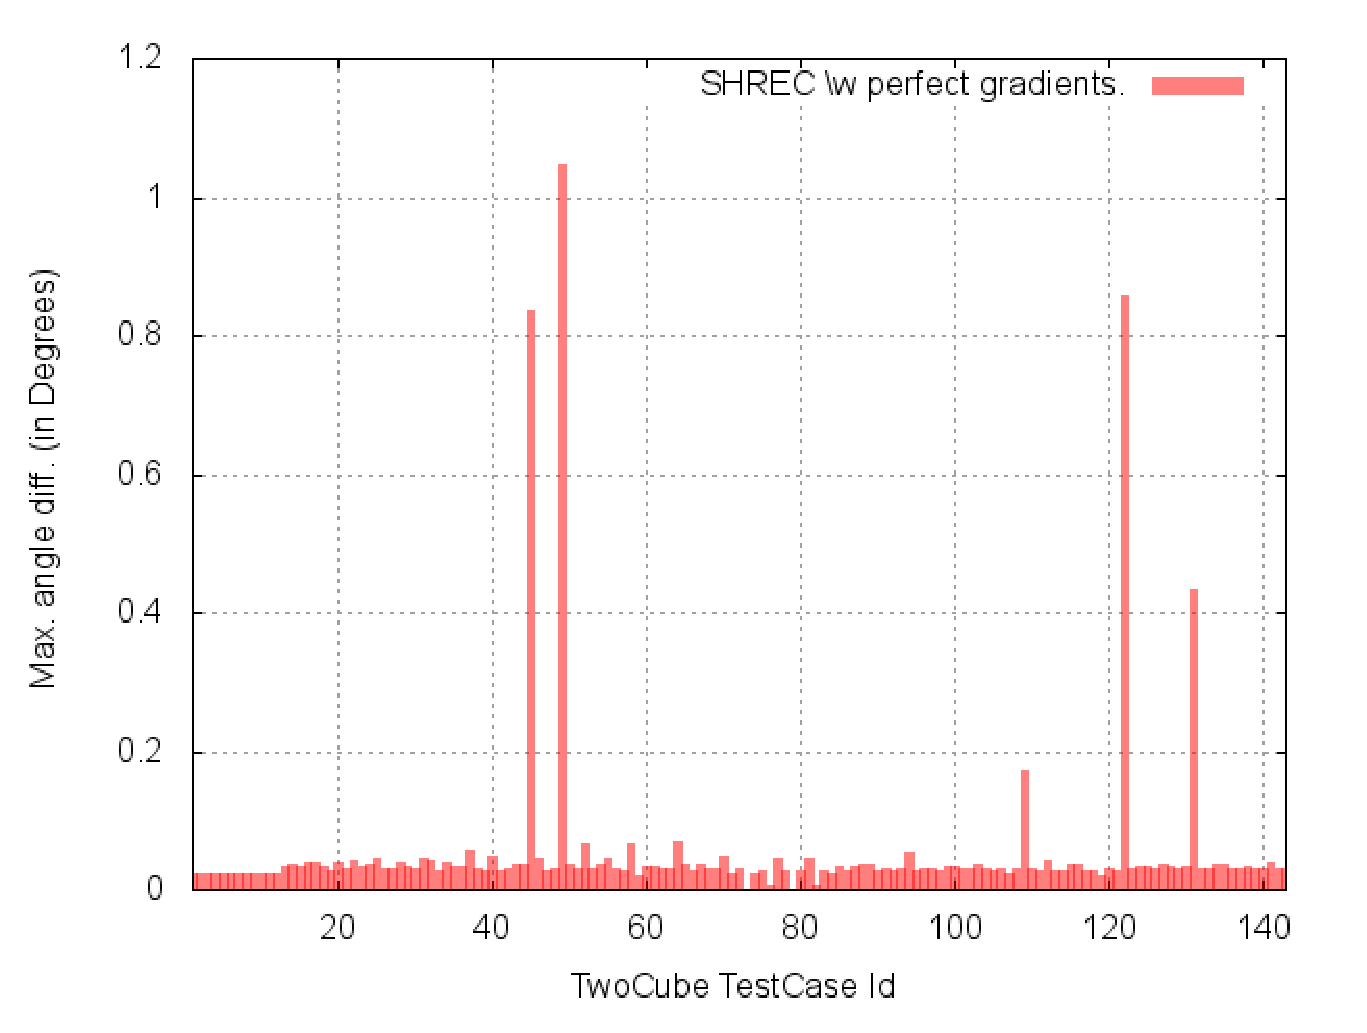
\includegraphics[width=0.3\linewidth]{images/shrecResCol3.eps}\label{fig:shrecTwoCube:b}}\\
	\subfloat[]{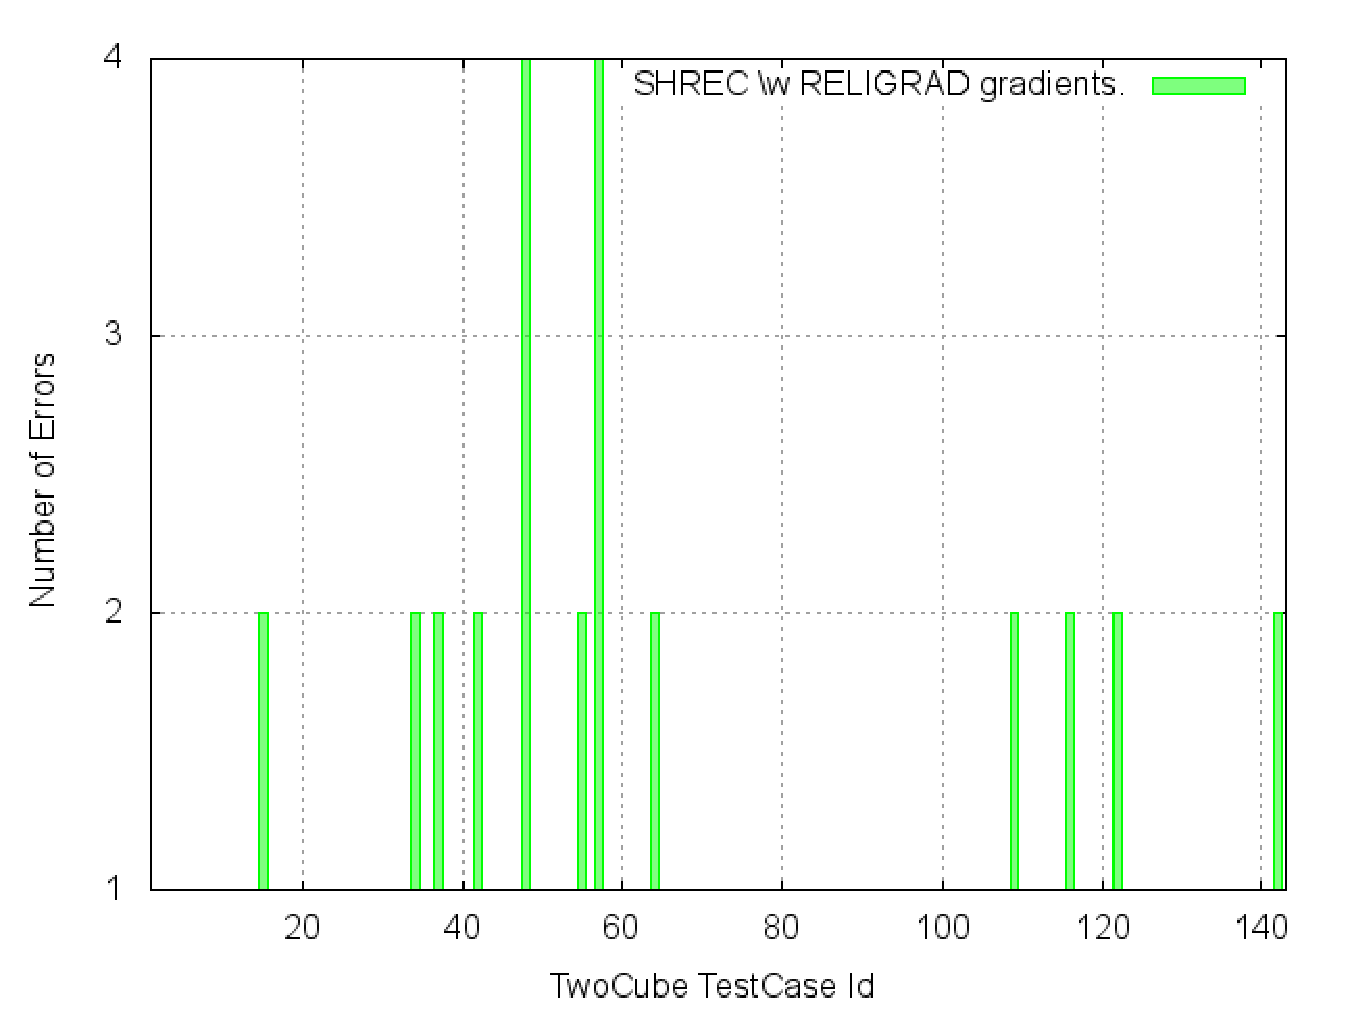
\includegraphics[width=0.3\linewidth]{images/shrecResCol2.eps}\label{fig:shrecTwoCube:c}}
	\subfloat[]{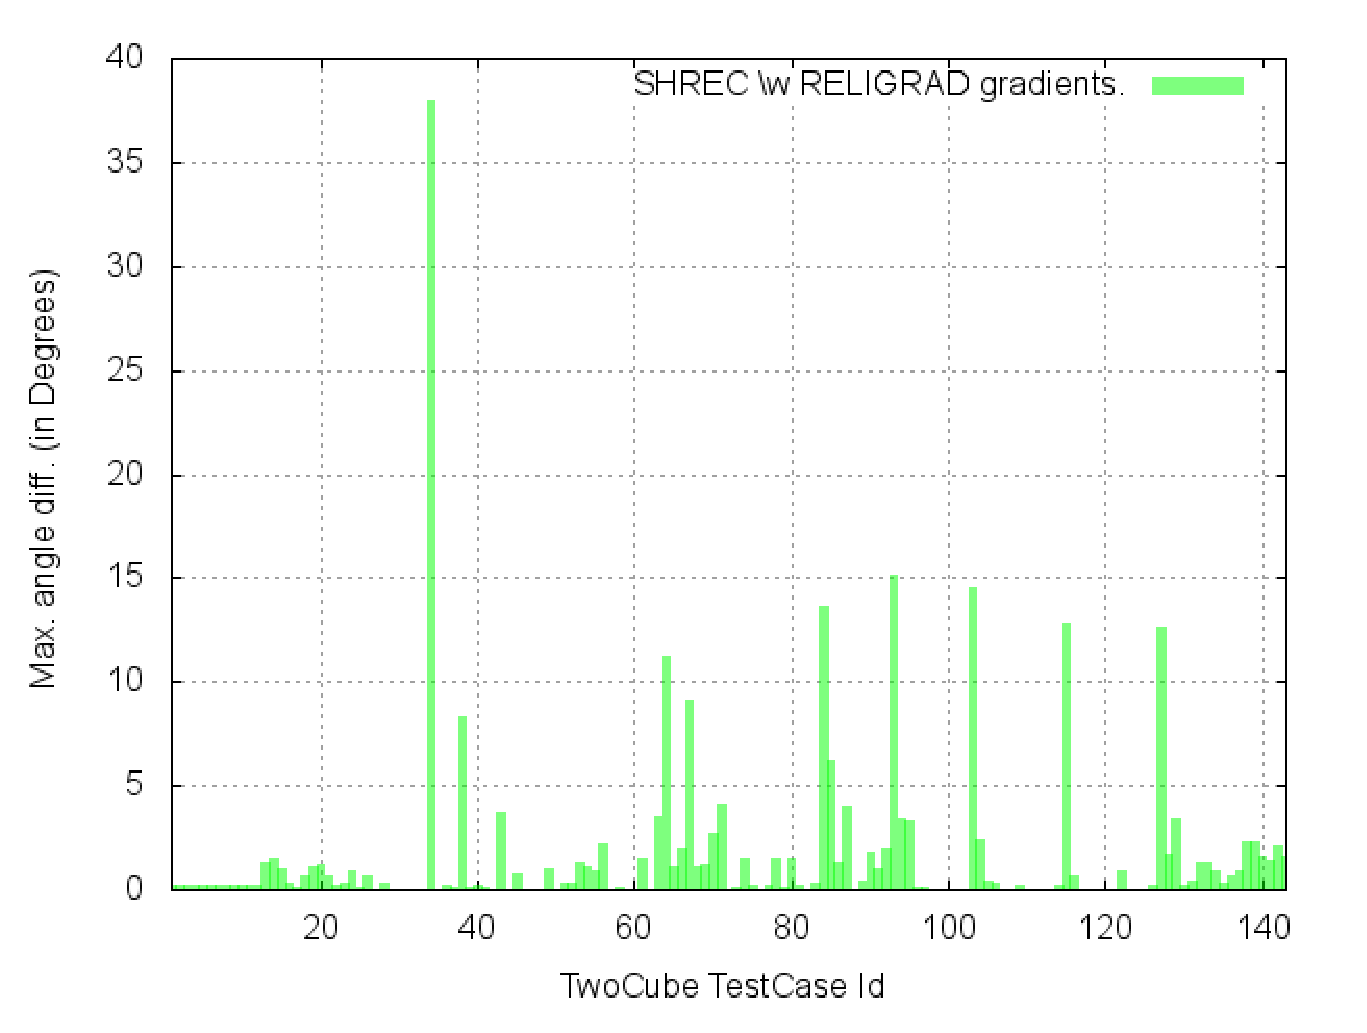
\includegraphics[width=0.3\linewidth]{images/shrecResCol4.eps}\label{fig:shrecTwoCube:d}}
	\caption{SHREC with perfect gradients and with RELIGRAD gradients(computed directly from scalar data.).~\protect\subref{fig:shrecTwoCube:a} shows the number of CountDegree errors when using SHREC along with the correct gradients.~\protect\subref{fig:shrecTwoCube:c} The same result when using gradients computed directly from scalar data (RELIGRAD). ~\protect\subref{fig:shrecTwoCube:b} shows the maximum angle difference from the ``perfect mesh" when using correct gradients.~\protect\subref{fig:shrecTwoCube:d} The same result when using RELIGRAD gradients. }
	\label{fig:shrecTwoCube}
	\vskip-0.2cm
\end{figure*}


We next ran SHREC on 143 TwoCube datasets; Figure~\ref{fig:shrecTwoCube} shows the summary results. As with Flange we first tested SHREC with synthetic gradients and then with gradients computed from the scalar data using RELIGRAD.

Figure~\protect\subref*{fig:shrecTwoCube:a} shows the number of CountDegree errors using the SHREC algorithm along with synthetic gradients at grid vertices as input. Only four test cases have errors, with the maximum having four errors. 
Figure~\protect\subref*{fig:shrecTwoCube:b}, shows the maximum angle difference from the original mesh. The maximum angle difference is 1.05 degrees for the dataset id 50.

Figure~\protect\subref*{fig:shrecTwoCube:c}, shows the CountDegree results using SHREC with RELIGRAD gradients. The maximum number of errors for a single dataset is four. Figure~\protect\subref*{fig:shrecTwoCube:d} shows the maximum angle difference from the original perfect mesh. While the maximum error was 38 degrees for a single test, majority produced very small errors. Figure~\ref{fig:shrecPerfect1} shows the mesh and the edges generated on a particular dataset.

Figure~\protect\subref*{fig:cannon:b},~\protect\subref*{fig:cannon:a} show our results of running SHREC with RELIGRAD on the Cannon datasets. Figure~\protect\subref*{fig:cannon:b} shows the CountDegree errors generated for the 15 cannon sets using gradients computed from RELIGRAD. The maximum error generated was 2. SHREC using synthetic gradients generated 'NO' errors. Figure~\protect\subref*{fig:cannon:a} shows one representative result using SHREC and RELIGRAD directly from scalar data. The magnified region shows a portion of the sharp edge. 

Similarly, Figure ~\protect\subref*{fig:cone:b},~\protect\subref*{fig:cone:a} show our results of running SHREC with RELIGRAD on the Cone datasets.
A single cone data set using synthetic gradients produces two Count Degree errors. With gradients computed from RELIGRAD the maximum number of errors is 4.
\begin{figure}[tb]
	\includegraphics[width=\linewidth]{images/shrecperfect.eps}
	\caption{Result of SHREC on a twoCube dataset. The FindSharp Edges are marked in red. Smooth edges are shown in cyan. The magnified region shows the output mesh edges around a corner.}
	\label{fig:shrecPerfect1}
\end{figure}
\begin{figure}[tb]
	\subfloat[]{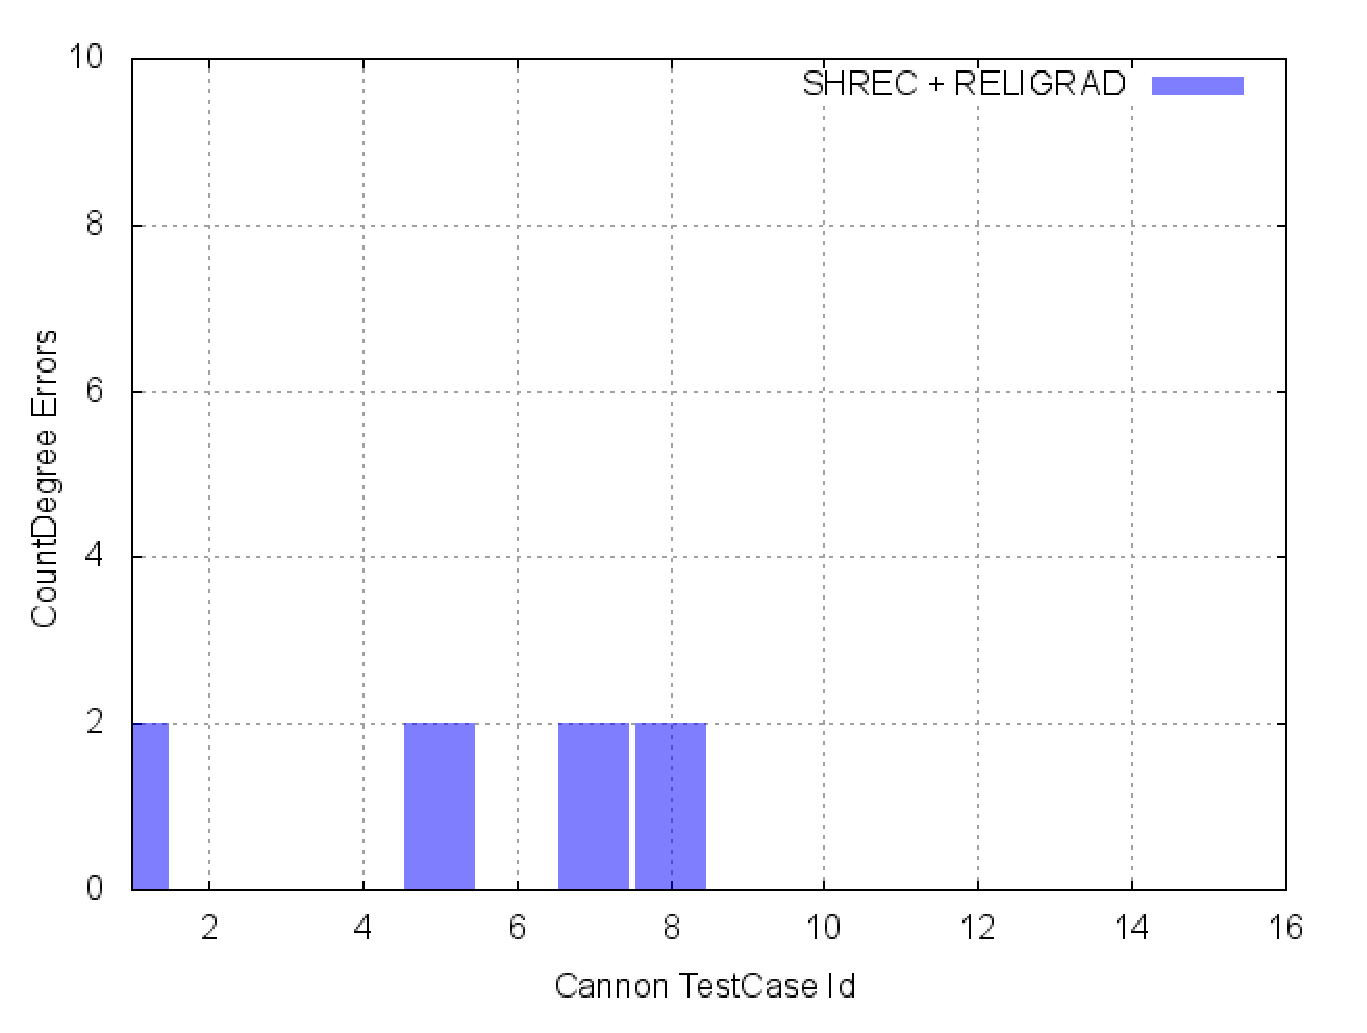
\includegraphics[width=0.5\linewidth]{images/cannon.eps}\label{fig:cannon:b}}
	\subfloat[]{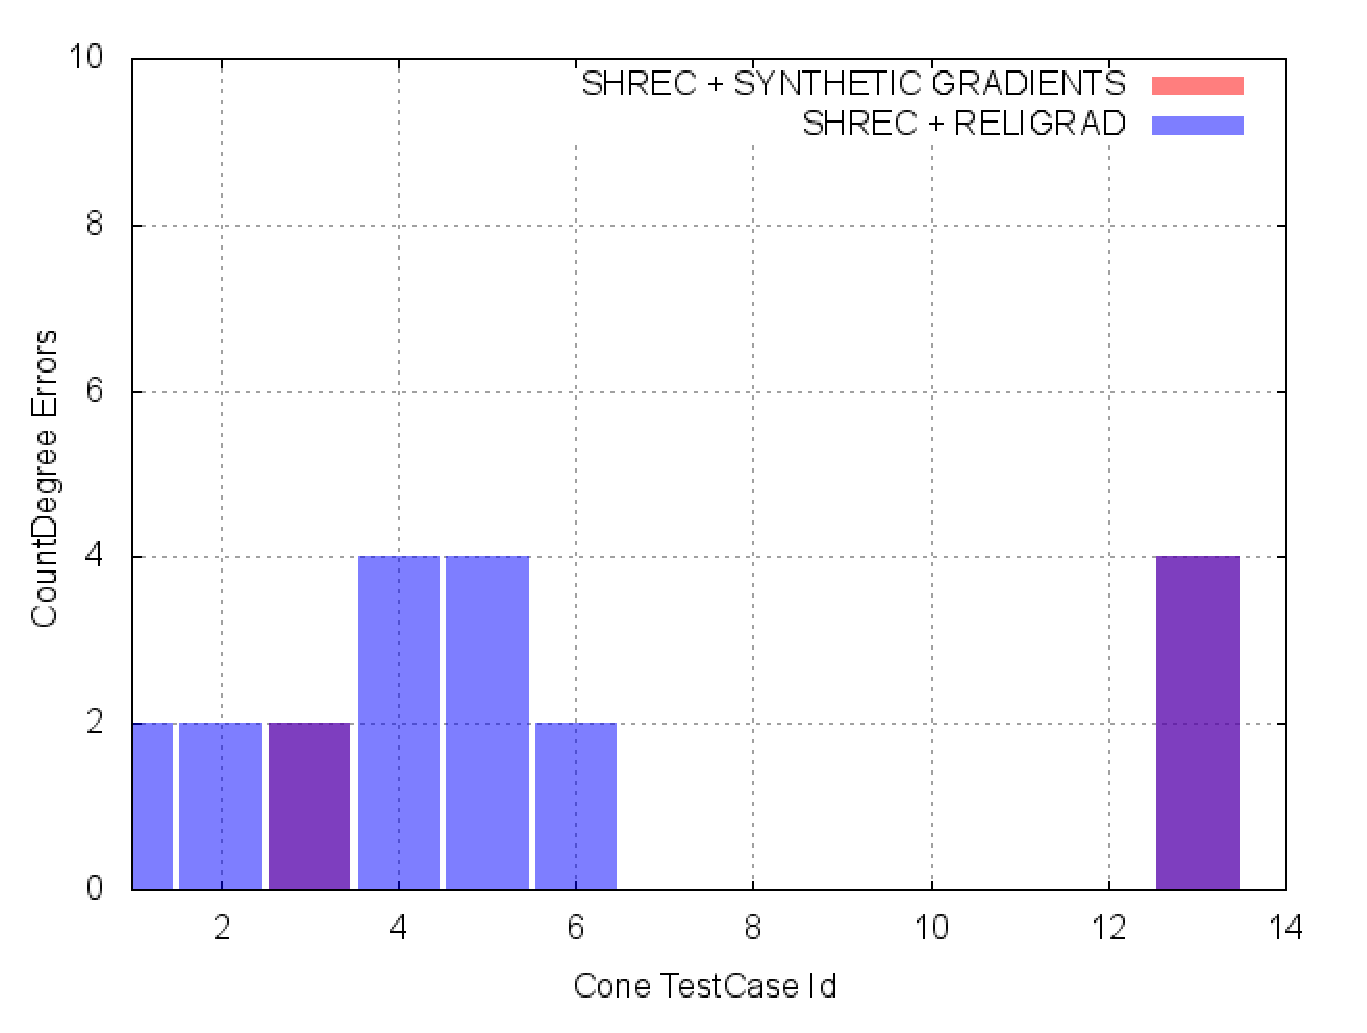
\includegraphics[width=0.5\linewidth]{images/cone.eps}\label{fig:cone:b}}
	\caption{Summary result of algorithm SHREC on Cannon and cone Datasets. (a) CountDegree Errors on 15 Cannon datasets using RELIGRAD gradients. SHREC with perfect gradients had no errors and is not shown. (b) CountDegree errors on 14 Cone datasets using RELIGRAD and perfect gradients.}
	\label{fig:cannon_cone_summary}
\end{figure}
\begin{figure}[tb]
	\subfloat[]{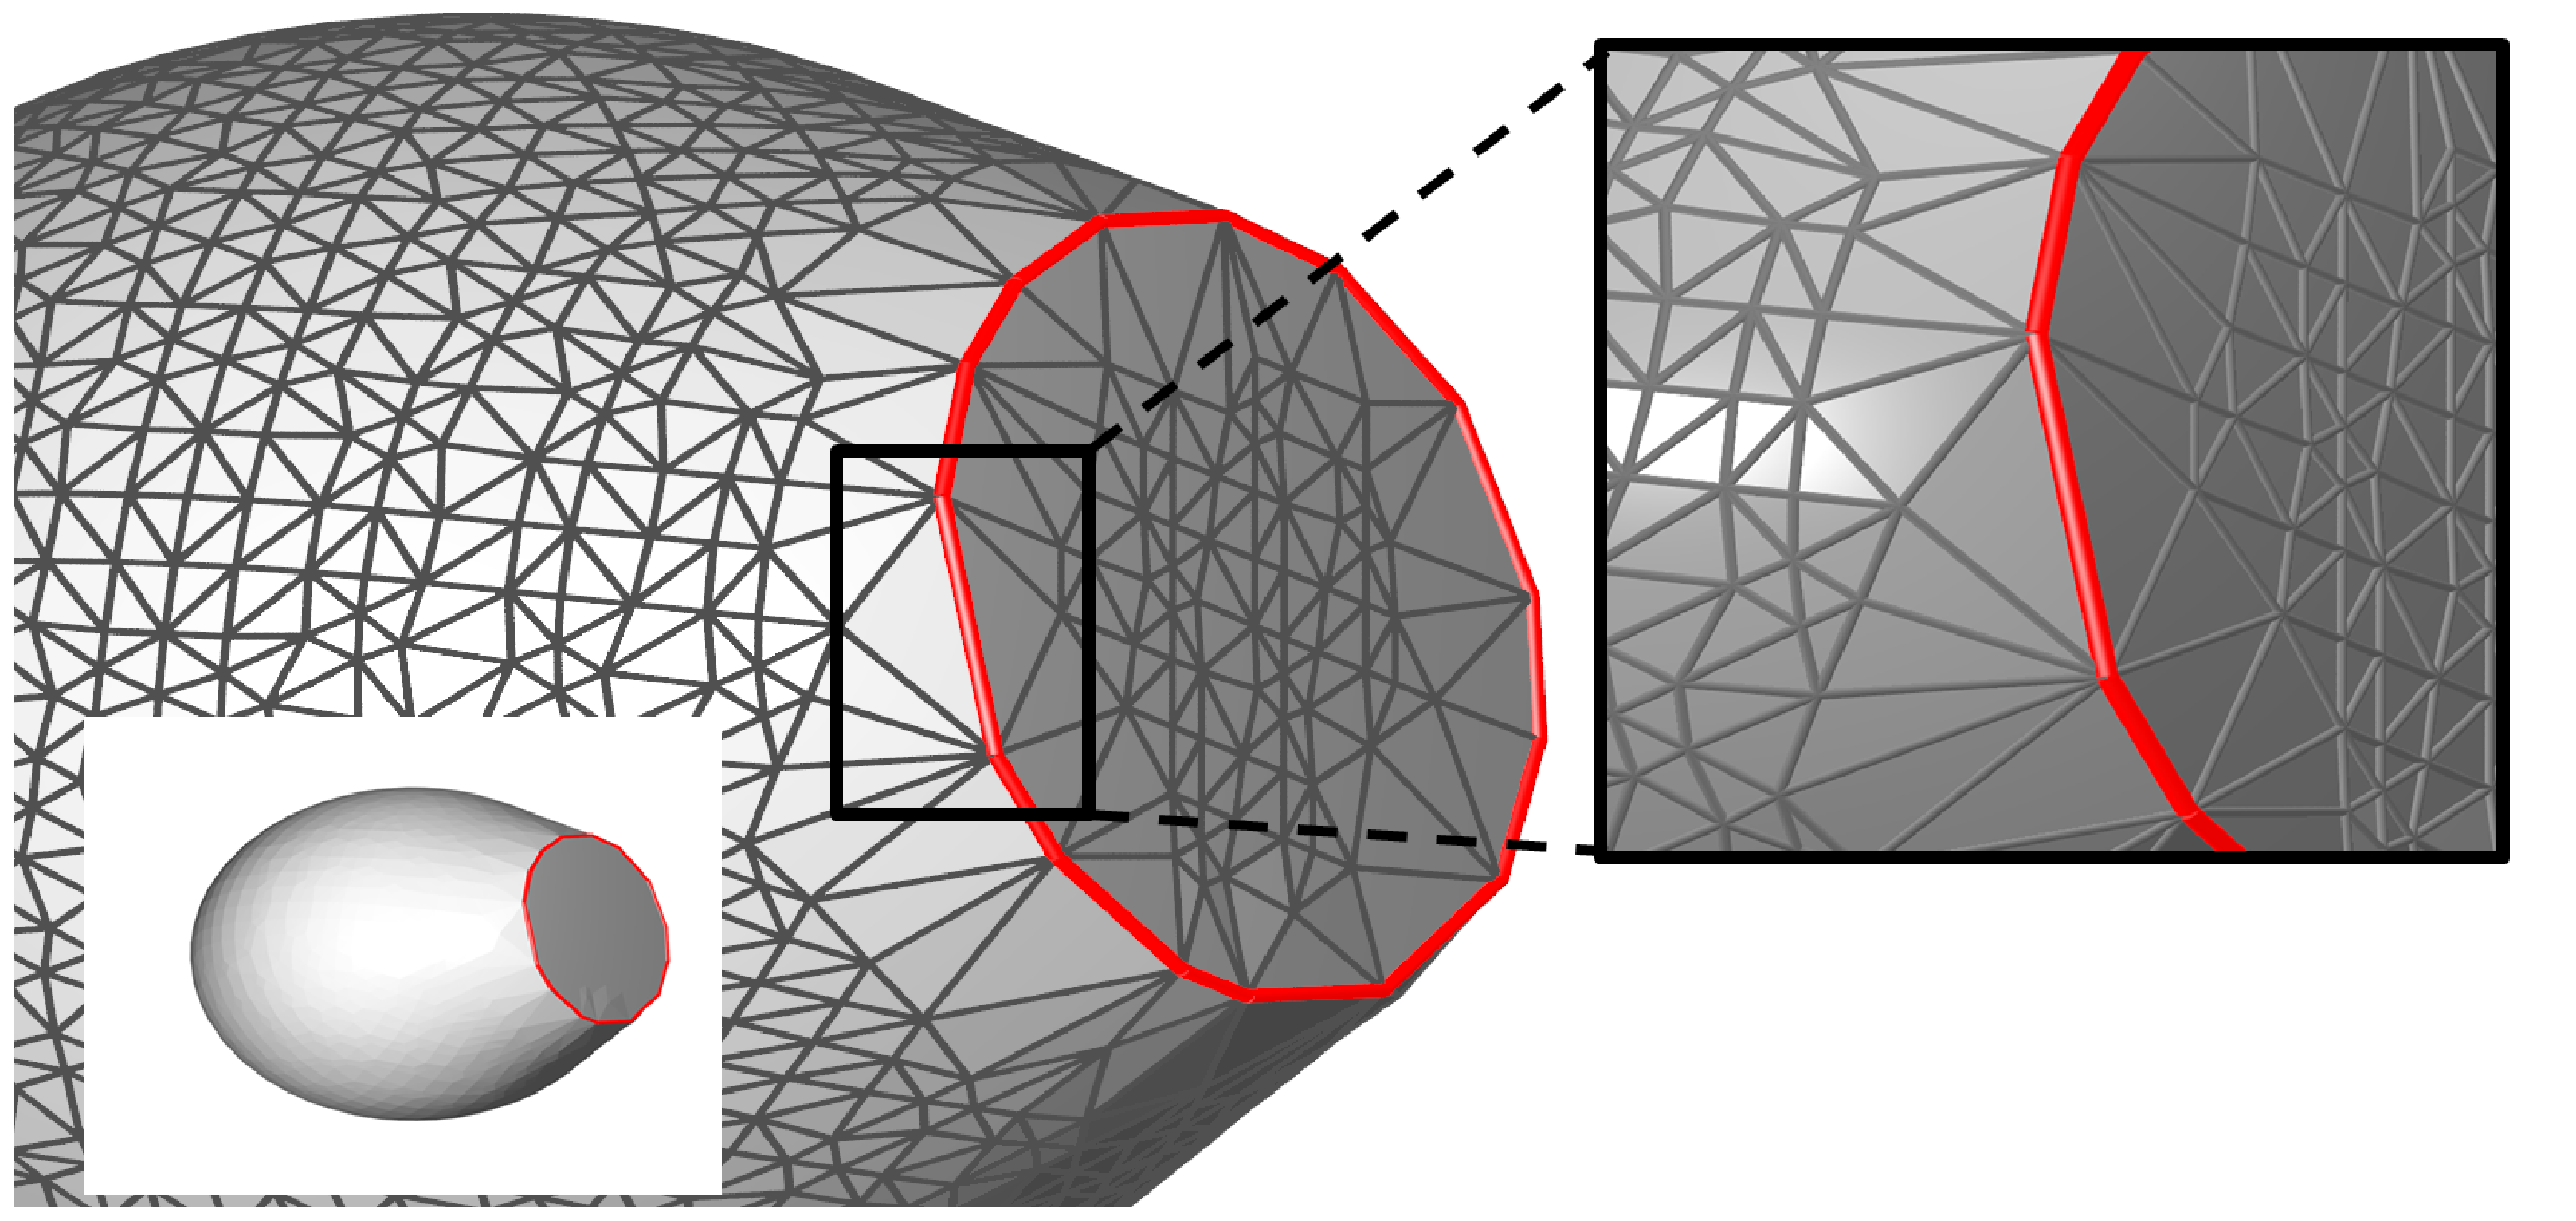
\includegraphics[width=0.5\linewidth]{images/cannon2.eps}\label{fig:cannon:a}}
	\subfloat[]{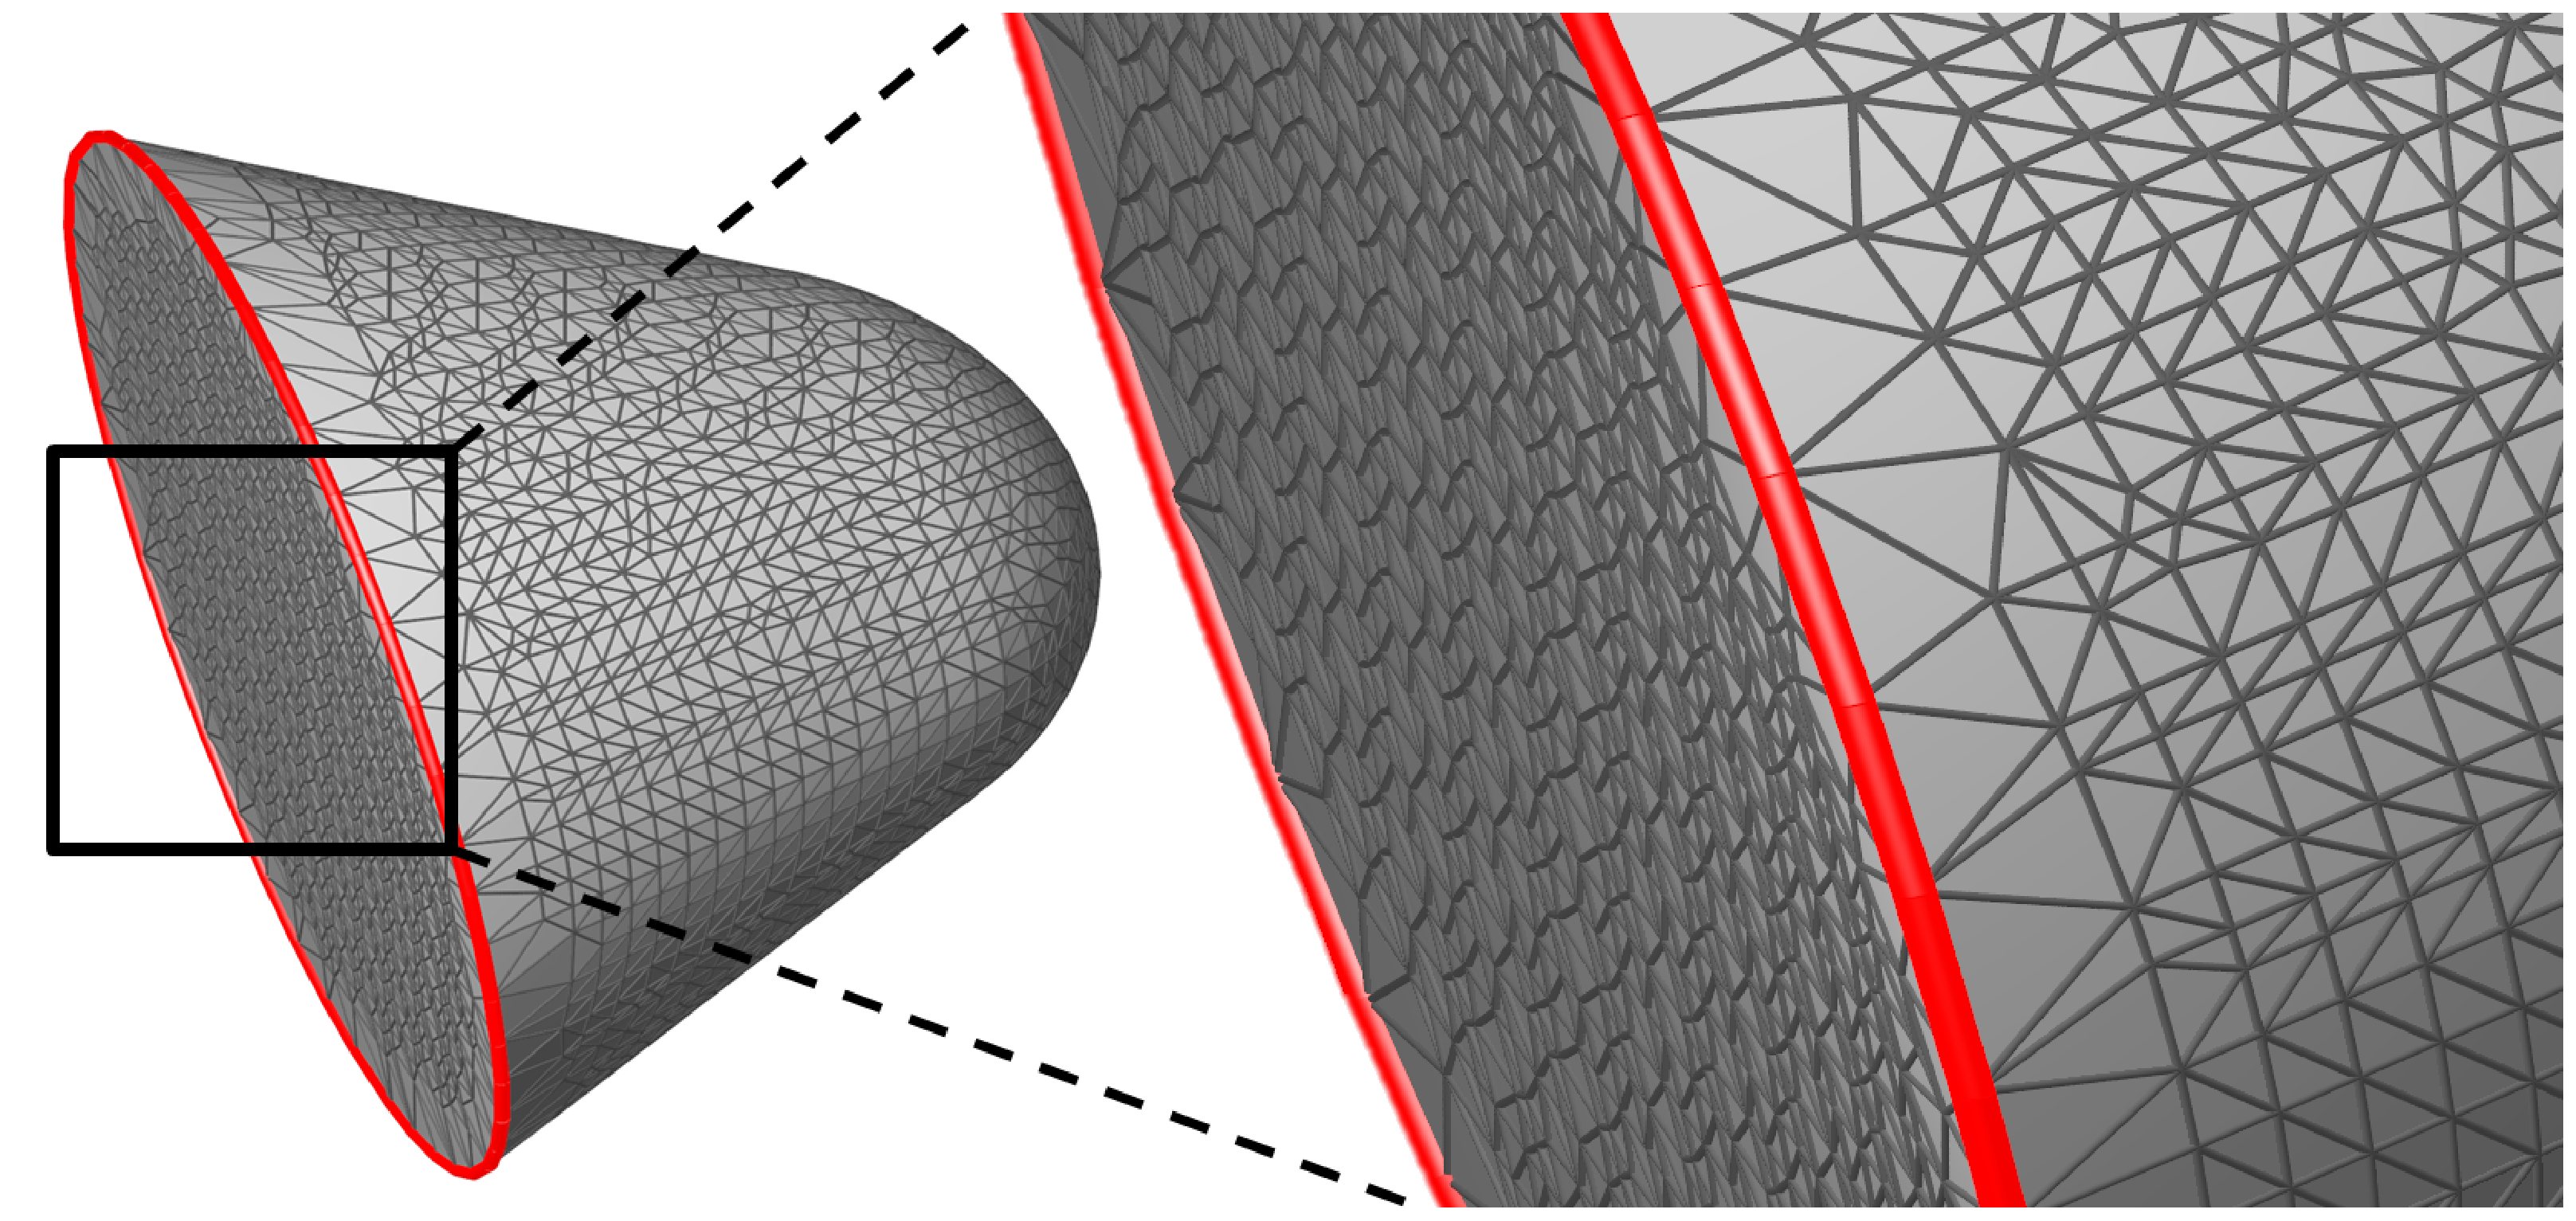
\includegraphics[width=0.5\linewidth]{images/cone2.eps}\label{fig:cone:a}}
	\caption{Result of algorithm SHREC with RELIGRAD gradients on Cannon and Cone datasets}
	\label{fig:cannon_cone}
\end{figure}
\section{Experimental Results on CT Data}

\subsection{Description of CT Data Sets}

\subsection{Comparison with Other Algorithms}
\paragraph{Comparison with MergeSharp}
%#150
\begin{figure}[htb]
	\centering
	\subfloat[]{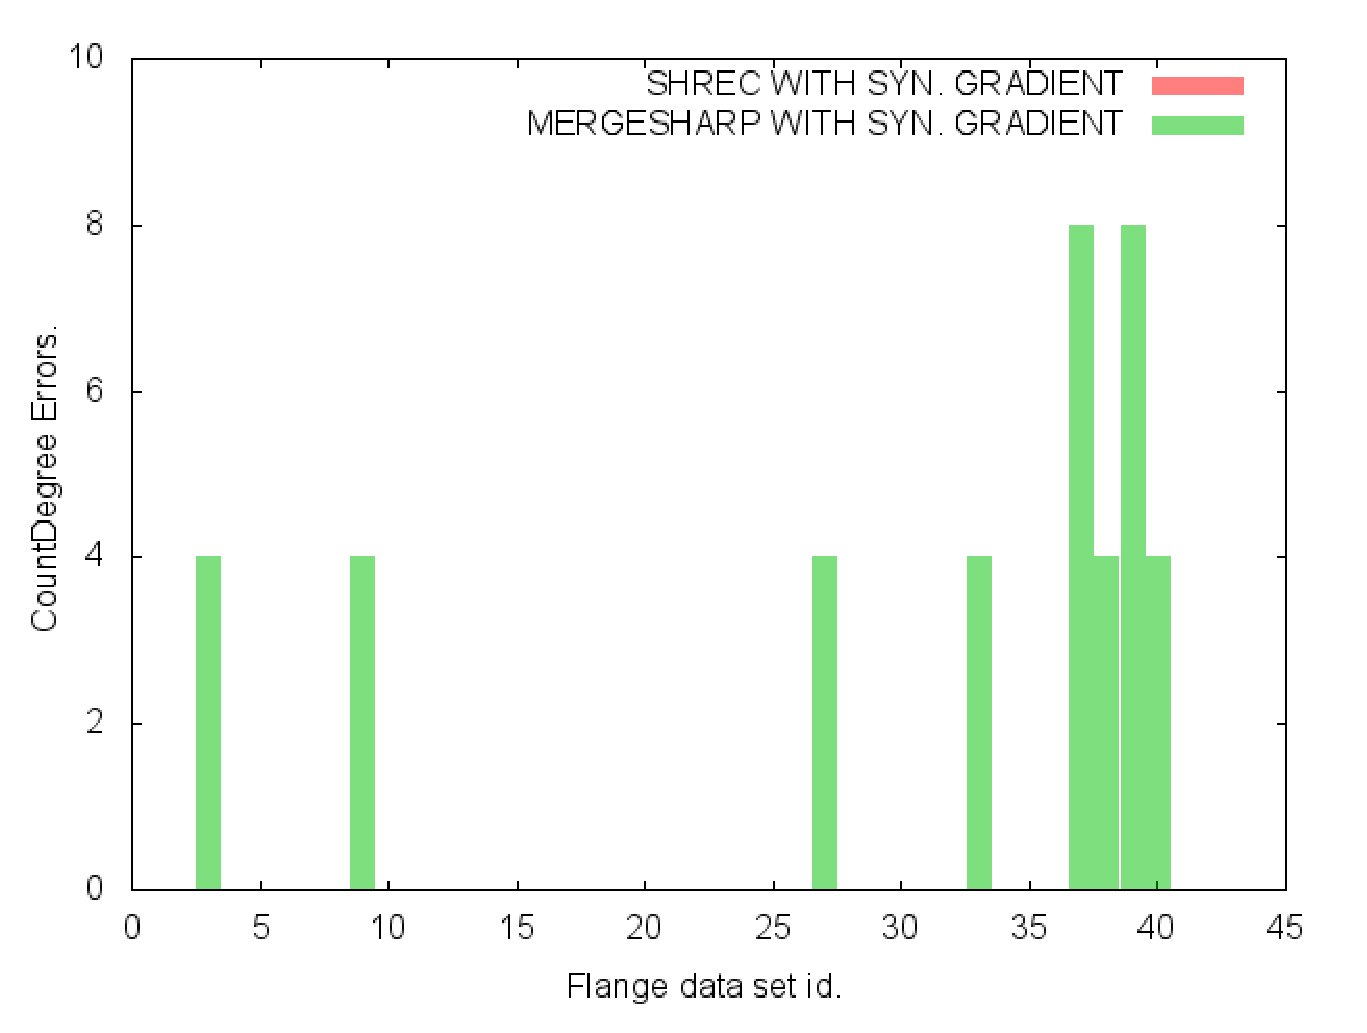
\includegraphics[width=0.8\linewidth]{images/mergeSharpvsShrec.eps}\label{fig:mergesharp:a}}\\
	\subfloat[]{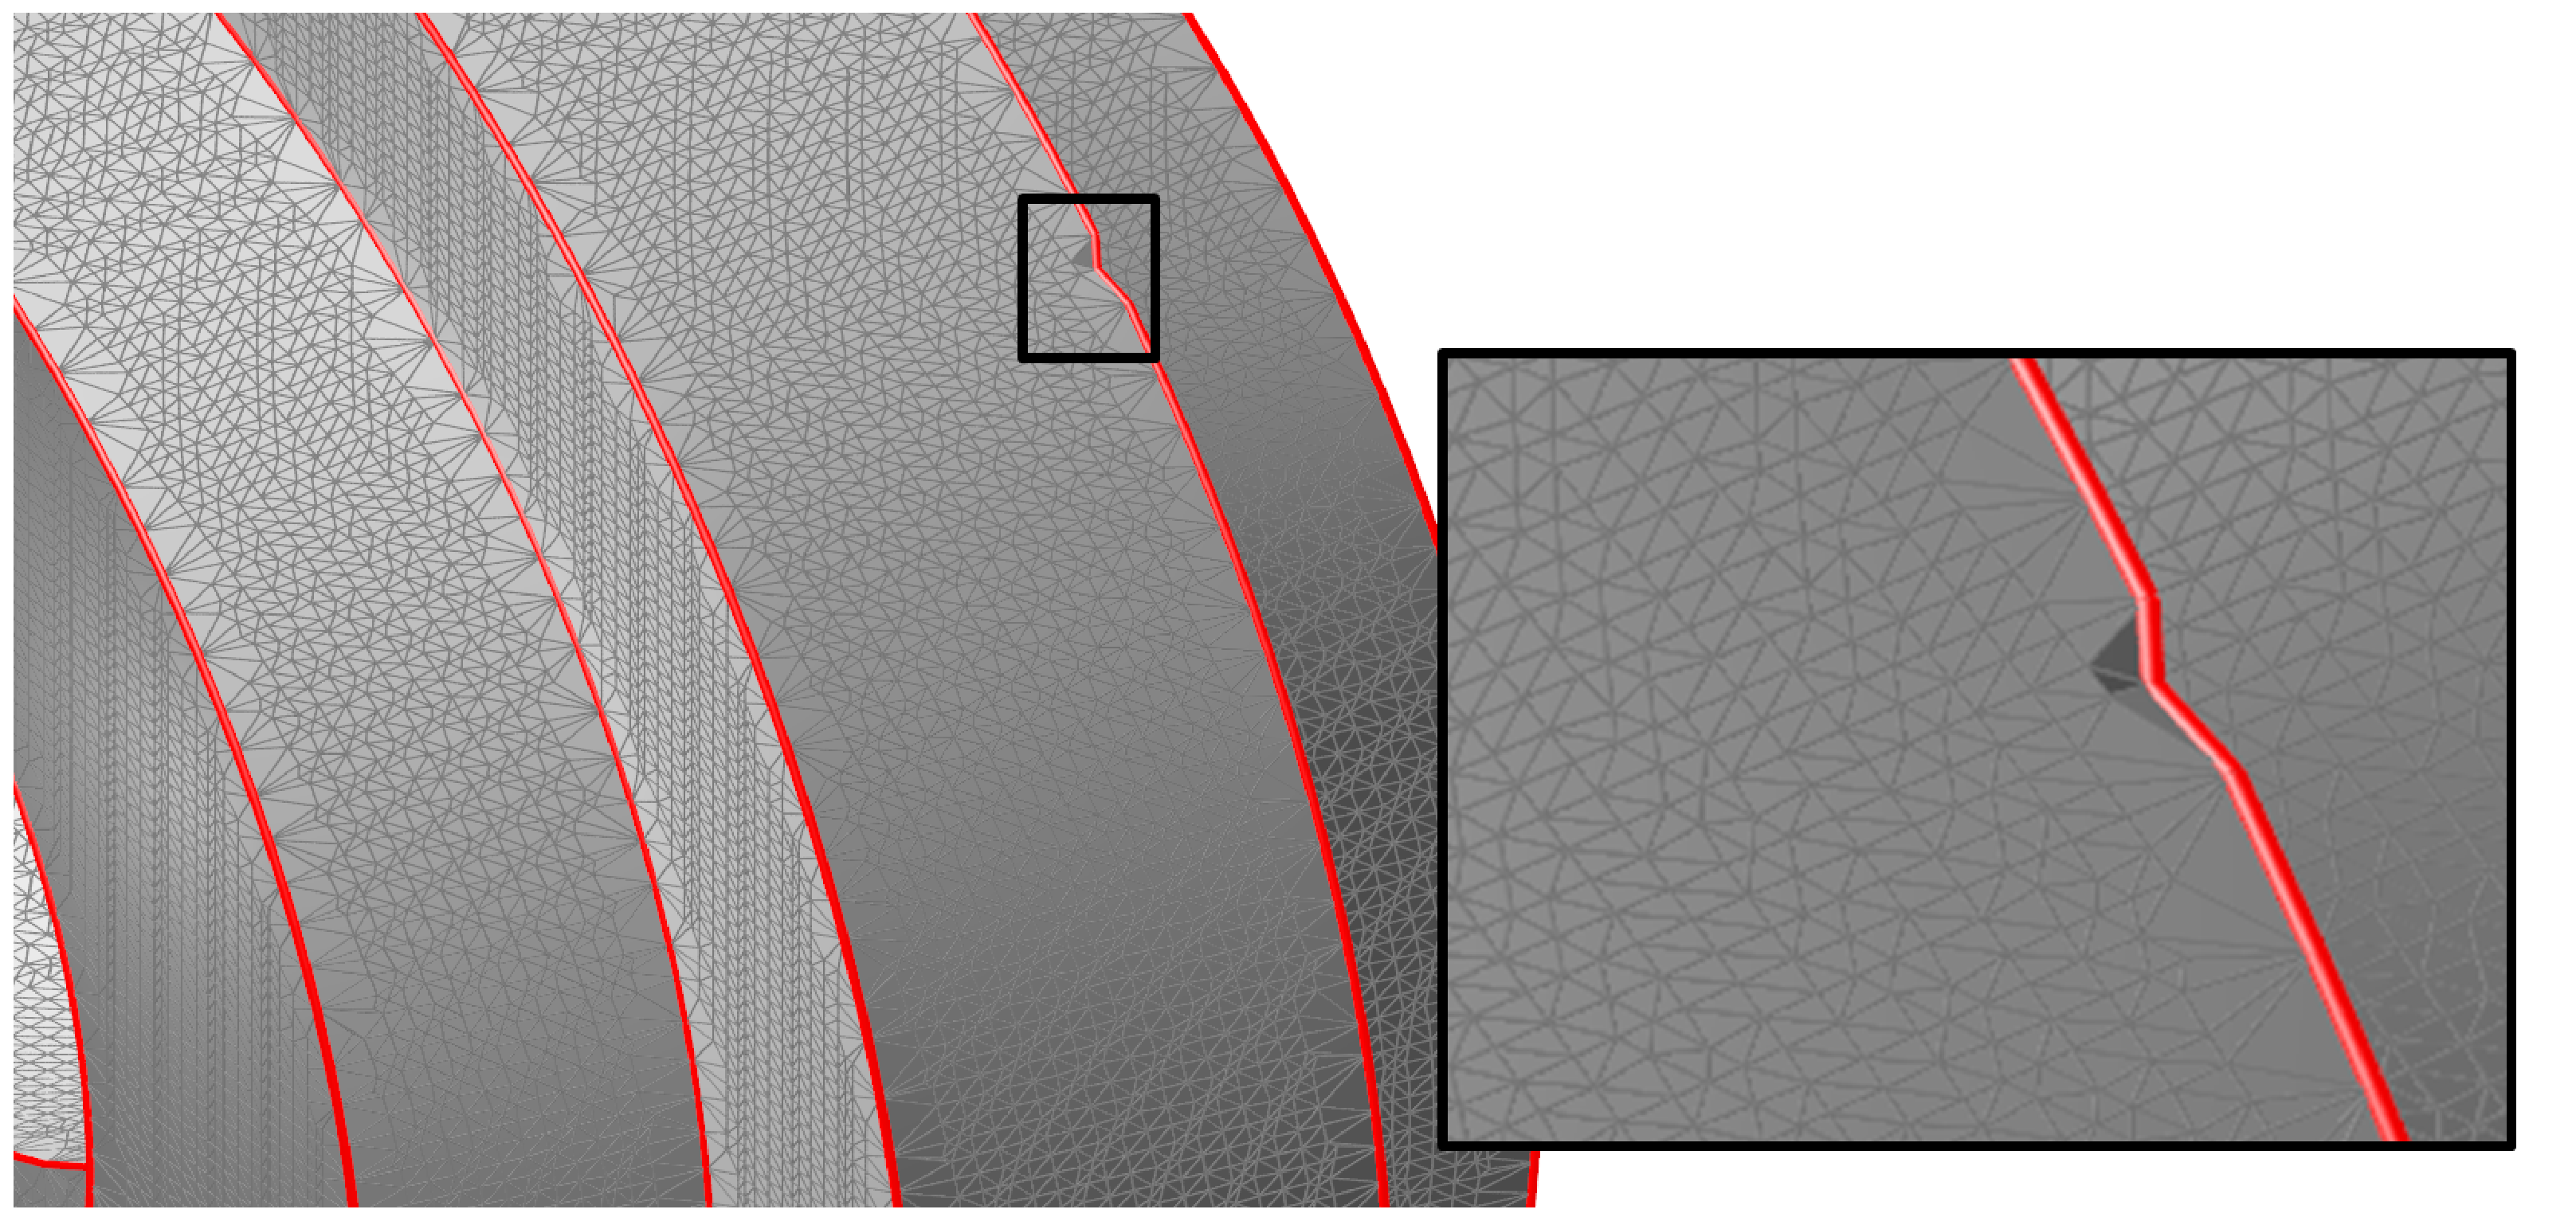
\includegraphics[width=0.6\linewidth]{images/mergeSharpvsShrec2.eps}\label{fig:mergesharp:b}}\\
	\subfloat[]{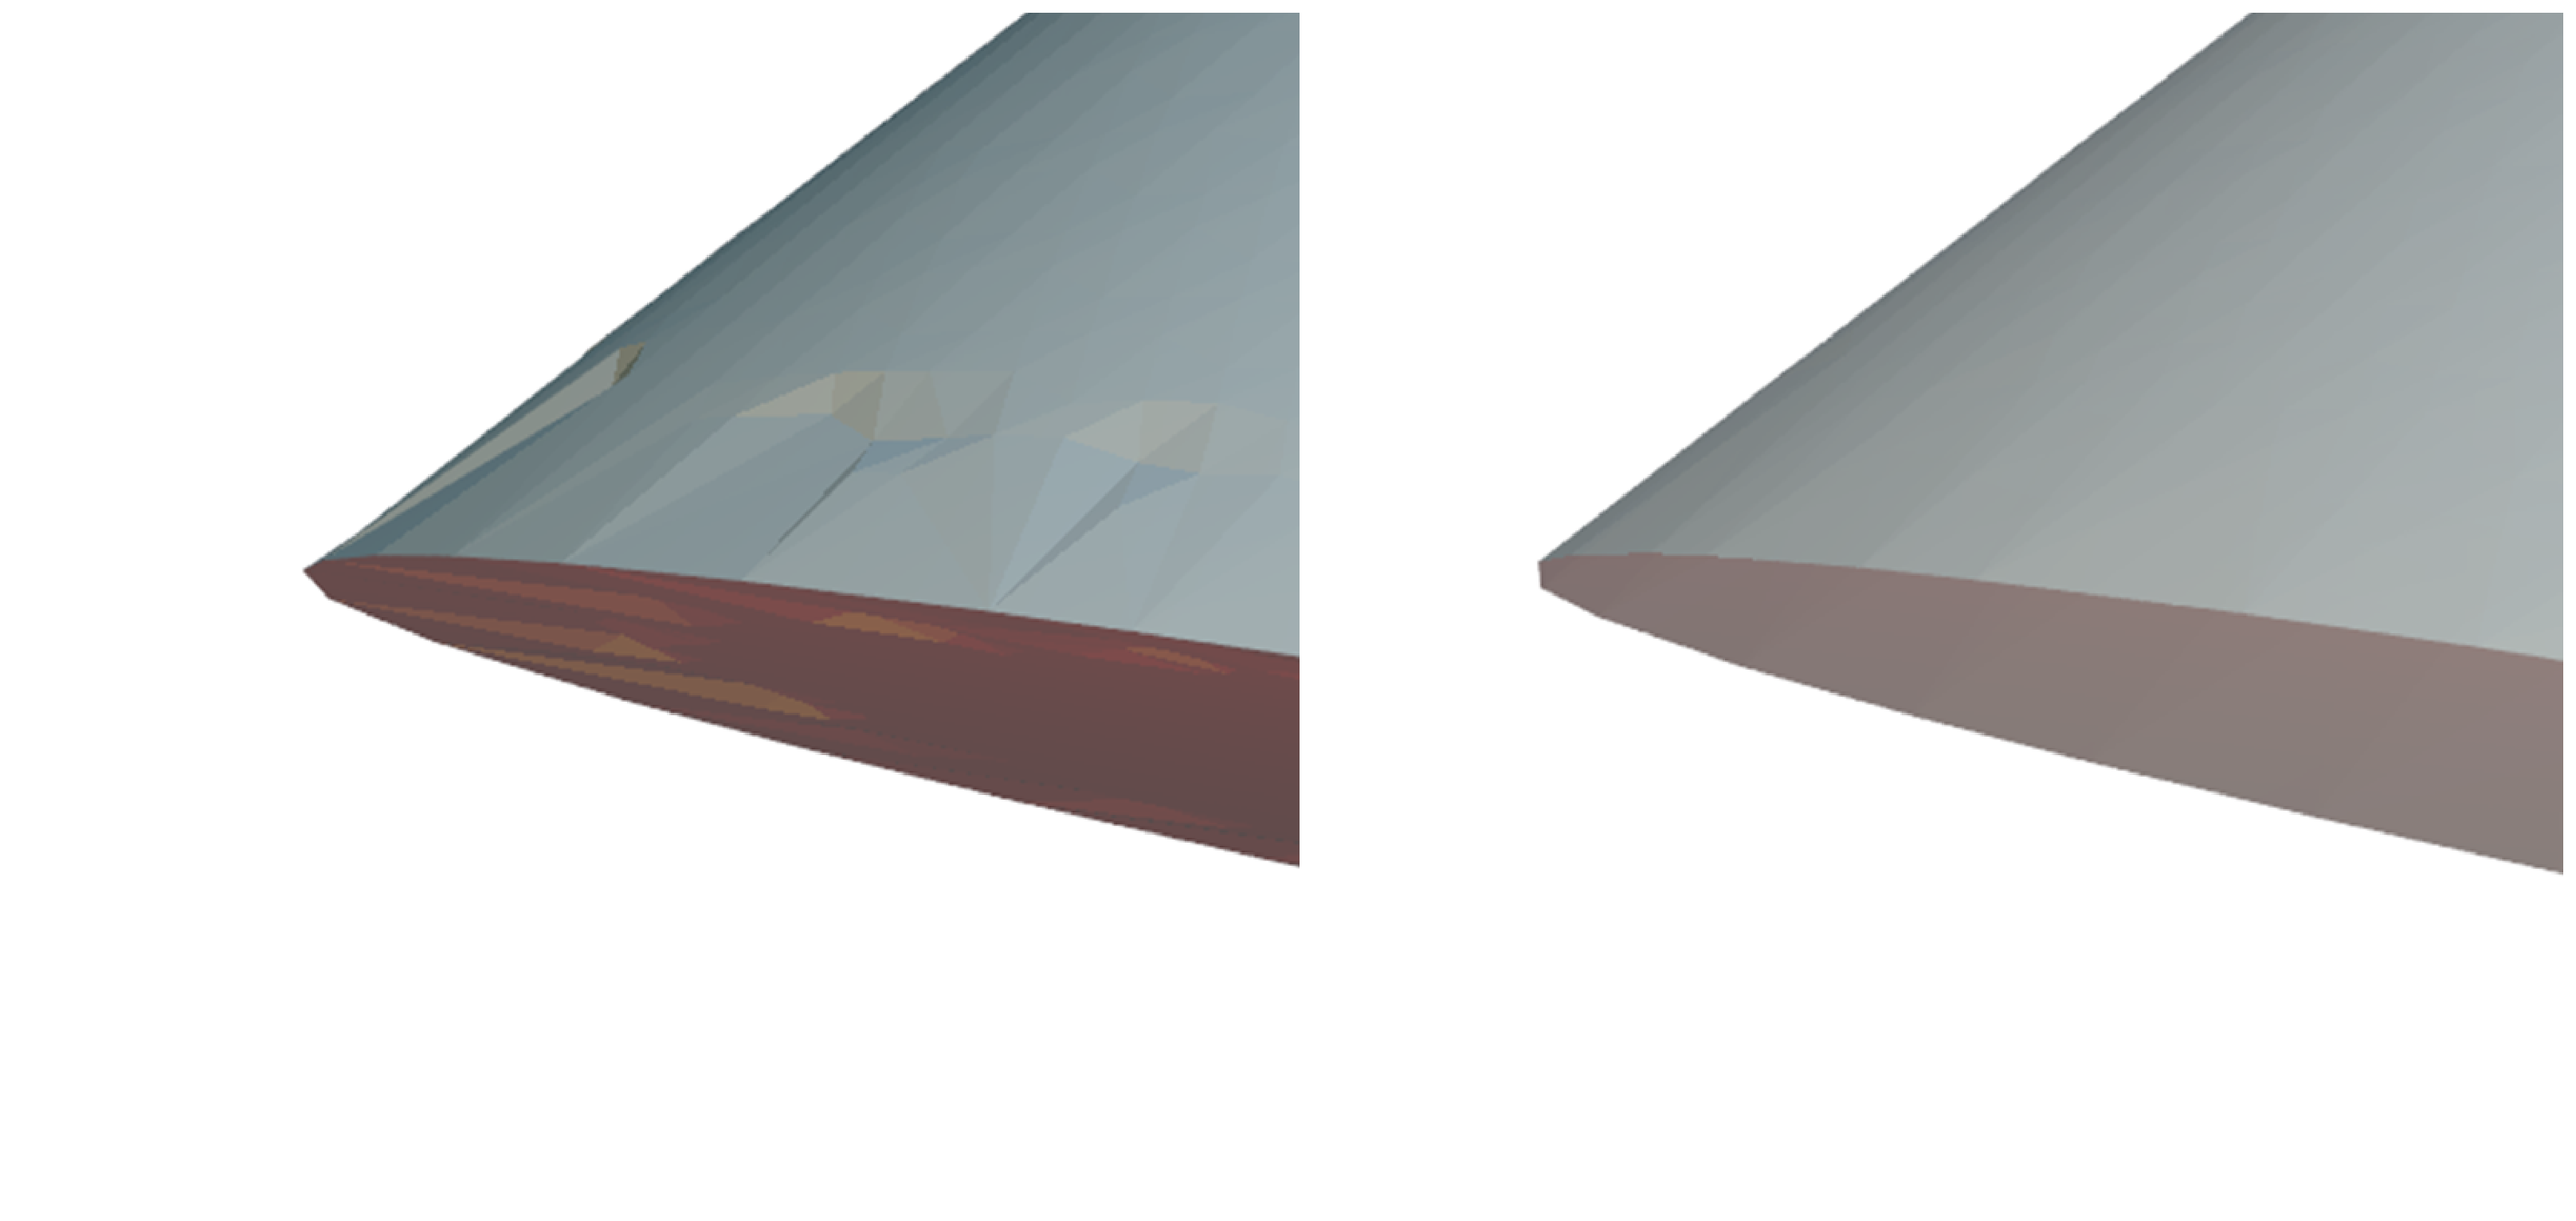
\includegraphics[width=0.6\linewidth]{images/cone_mergesharp.eps}\label{fig:mergesharp:c}}
	\caption{Result of  MERGESHARP and SHREC with synthetic gradients. (a) Summary results of  CountDegree errors of 40 Flange datasets. SHREC does not produce an errors. (b) Result on one particular data set using MERGESHARP, magnified region shows one of the ``notches" created. (c) Apart from ``Notches", MERGESHARP produces gentle dimples which decays the visual quality. Magnified region shows a portion of a Cone dataset (Left) MERGESHARP (Right) SHREC. }
	\label{fig:mergeSharpVShrec}
\end{figure}	
We first compare our algorithm with MERGESHARP ~\cite{bw-cisec-13}, Figure~\ref{fig:mergeSharpVShrec} shows the result. Figure~\protect\subref*{fig:mergesharp:a} shows the summary of CountDegree results of running MERGESHARP on 40 Flange datasets. SHREC as discussed above does not generate any errors. Figure~\protect\subref*{fig:mergesharp:b} shows the result on one of the Flange data sets. MERGESHARP produces ``notches" such as the one shown. 

MERGESHARP also produces gentle dimples such as the ones in the edge of a Cone data set shown in Figure~\protect\subref*{fig:mergesharp:c}, SHREC does not produce them. 	
\paragraph{Comparison with Cocone}
We compare our algorithm to the algorithm WeightCocone by Dey et al.~\cite{Dey2012}. WeightCocone reconstructs a surface with sharp edges and corners from a sampled point cloud. WeightCocone takes two inputs; one contains the point cloud, another is a weighted sampling of feature curves. Weight of the sampling will be used as weight of the protecting balls. WeightCocone generates as output a feature sensitive mesh. 

The feature curve (second input to WeightCocone) is constructed using the algorithm FeatureRecon by Dey et al.~\cite{Dey2013}. FeatureRecon extracts feature curves of a surface. The input is a point cloud sampled on the surface. FeatureRecon has two steps, feature point detection and feature curves reconstruction. 
\paragraph{Experimental details:} The input to FeatureRecon is a point cloud. We tested two different input point cloud;
\begin{enumerate}
	\item We applied Marching Cubes~\cite{lc-mchr3-87} on our datasets Sec.\ref{sec:synData}. The vertices of the mesh generated by the Marching Cubes algorithm are then super-sampled using the Monte Carlo point sampling, to generate a point cloud with approximately sixty-five thousand points.
	\item We super-sampled the ``perfect" meshes Sec.\ref{sec:synData}, to generate generate a point cloud with approximately sixty-five thousand points.
\end{enumerate}
The two different point clouds are used as input to FeatureRecon to extract the feature curves. 
FeatureRecon has nine separate parameters. Experimentally and also noted by the authors Dey et al.~\cite{Dey2013}, we found FeatureRecon to be heavily reliant on parameter fine tuning. We used the following parameter values for our TwoCube datasets, (as suggest by the authors Dey et al.~\cite{Dey2013}). 
$-t = 25,-fl = 0.04, -cl = 0.06, -dc = 0, -\rho3 = 0.32, -\rho1 = 0.0, -rc = 3$.

The feature curves generated using FeatureRecon along with the super-sampled point cloud is used as input to WeighCocone. For comparison test, we compare the known ``perfect" mesh with the output of WeightCocone. 
We report the degree count of the ``sharp" edges (dihedral angle less than $140^\circ$). We also report the surface angle distances between the output and the perfect mesh. 
\begin{figure}[t] 
	%dataset t110 reconstructed from perfect mesh 
	\centering  	
	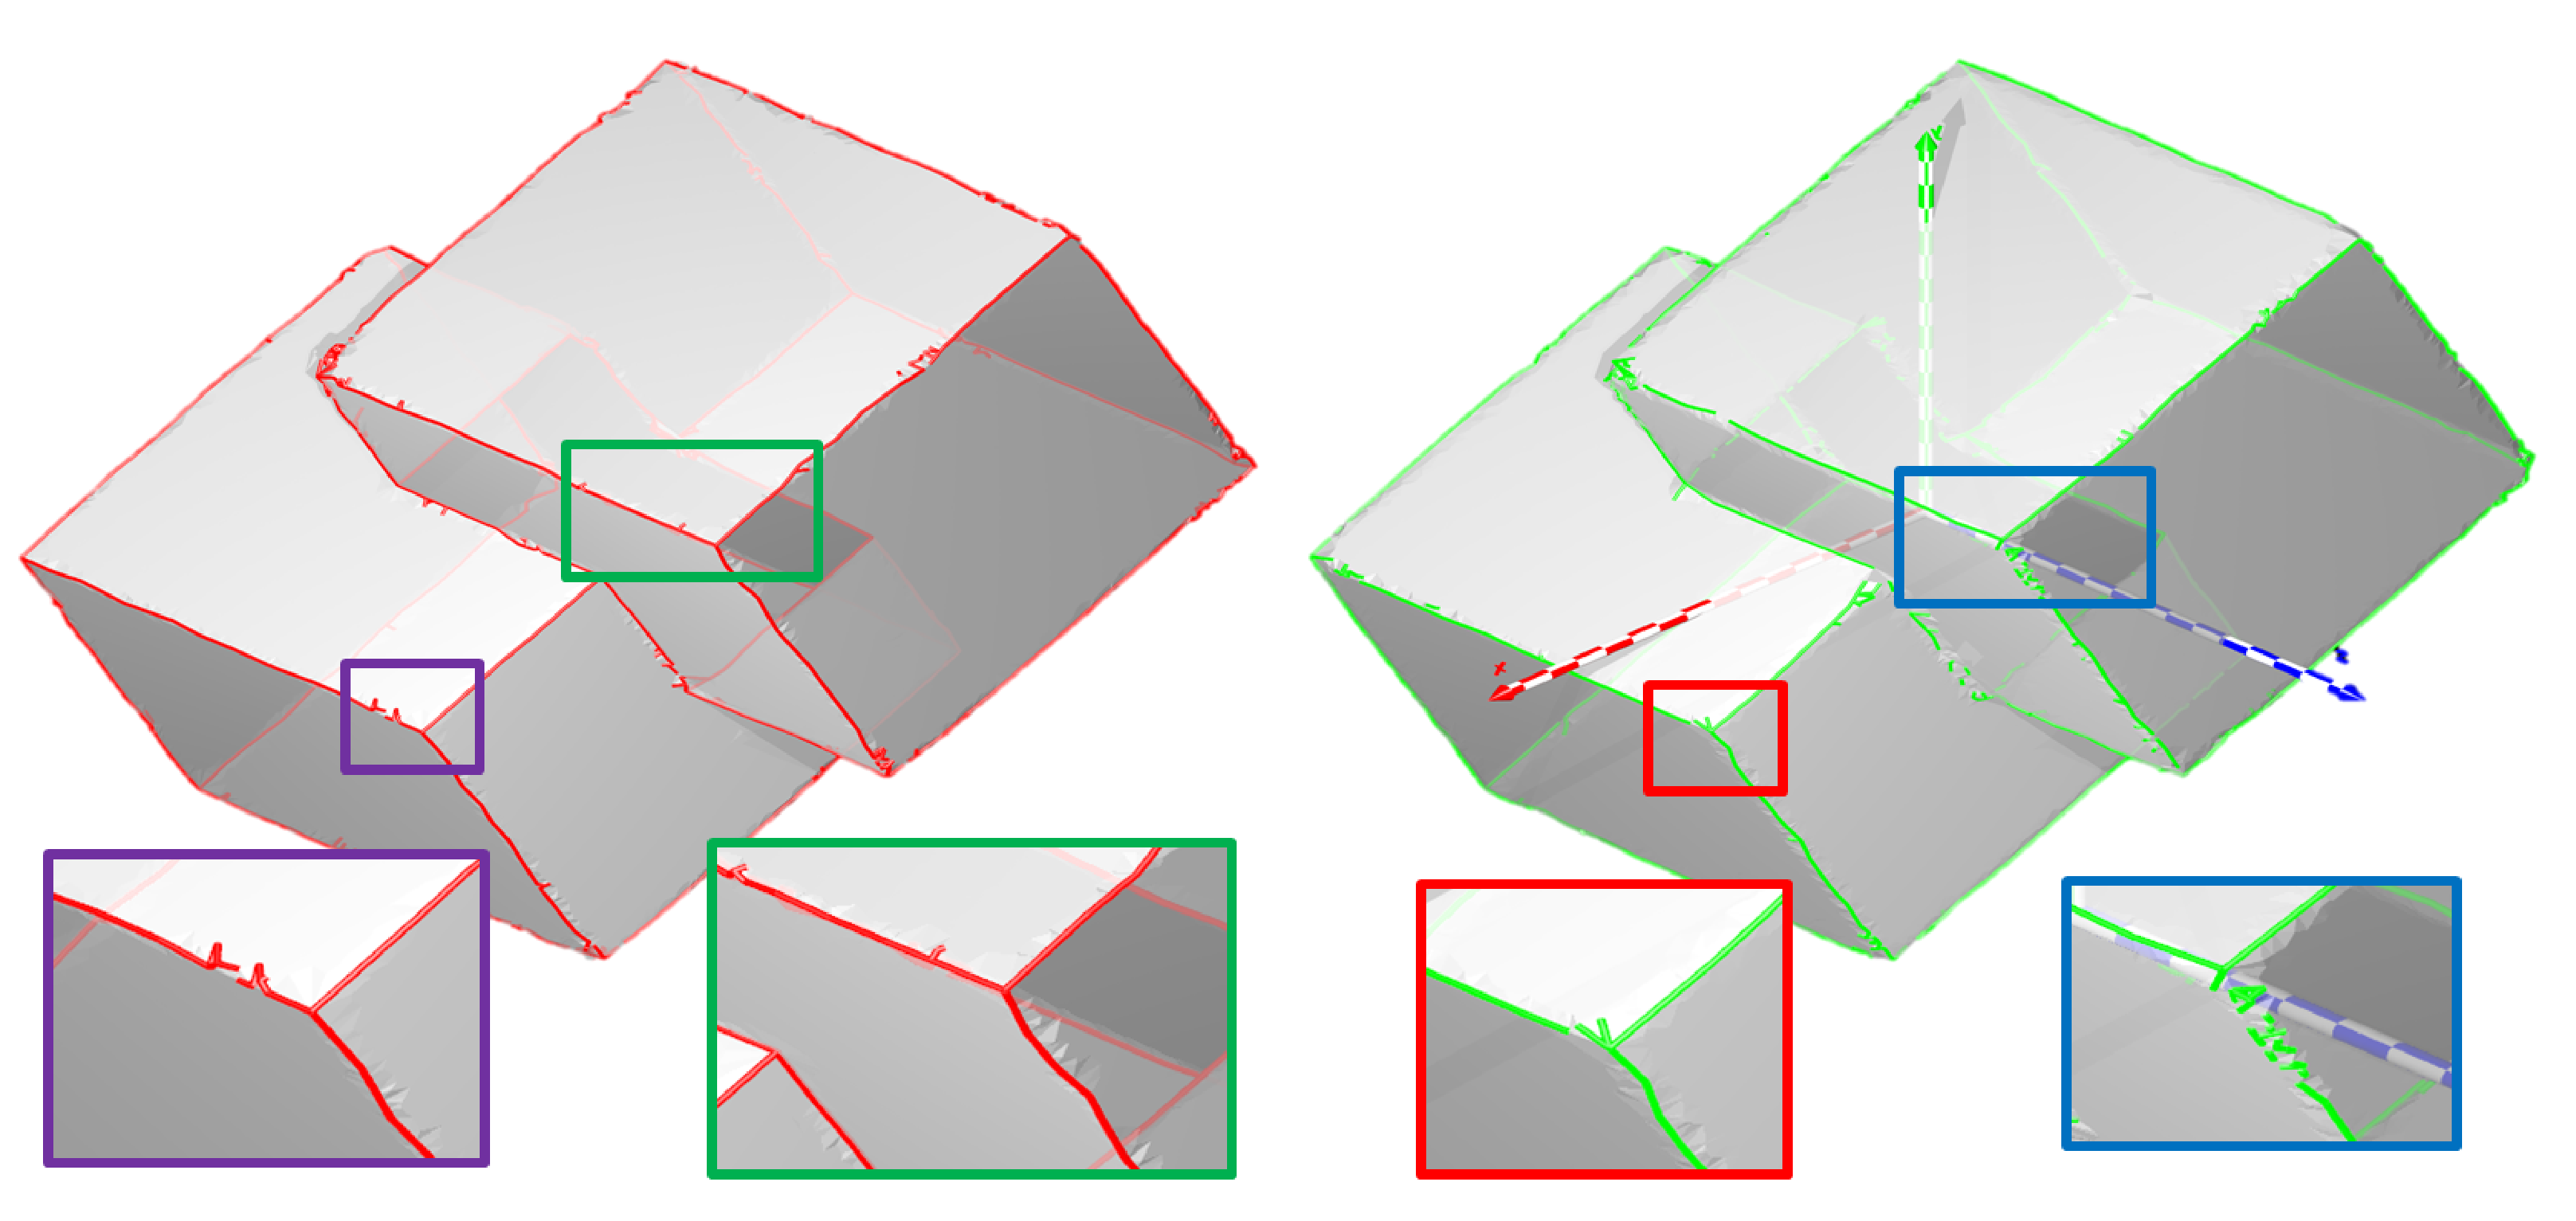
\includegraphics[width=\linewidth]{images/compare_cocone_perfect_mc.eps}
	\caption{Result of WeightCocone reconstruction on a TwoCube dataset (id 110). (a) Input cloud is the super-sampled ``perfect" mesh. (b) Input cloud is the super-sampled Marching Cube mesh. The magnified regions show some of the errors. The reconstruction from point cloud generated from the Marching Cube input is worse than the  point cloud from ``perfect" mesh input. }
	\label{fig:cocone_compare_from_perfect_1}
	\vskip-0.2cm
\end{figure} 
Figure~\ref{fig:cocone_compare_from_perfect_1} shows the reconstructed mesh for dataset id 110. The associated ``sharp" edges are also shown. Figure~\ref{fig:cocone_compare_from_perfect_1}(a) shows the reconstruction from the point cloud generated from the ``perfect" mesh. The overlay-ed ``sharp" edges (in red) show that the reconstruction has many errors. The magnified regions show some of the errors along the sharp edges and corners. Figure~\ref{fig:cocone_compare_from_perfect_1}(b) shows the reconstruction from the point cloud generated from running Marching Cubes. The magnified regions show the same regions as Figure~\ref{fig:cocone_compare_from_perfect_1}(a). The reconstruction is worse than WeightCocone using input from perfect mesh. 

Figure~\protect\subref*{table:cocone_compare_with_mc_table_2} shows the angular difference from the ``perfect" mesh to those generated by WeightCocone using points sampled from the ``perfect" mesh,  over a randomly selected subset of 21 cases out of the 143 TwoCube datasets. The number of simplices with more than 30$^\circ$, 40$^\circ$ and 50$^\circ$ errors from the original mesh are shown. Figure~\protect\subref*{fig:shrecTwoCube:a},~\protect\subref*{fig:shrecTwoCube:c} show that algorithm SHREC generates far fewer errors and with smaller angle difference to the original mesh. WeightCocone when using Marching Cubes point cloud as input produces worse results and is not shown.

Figure~\protect\subref*{table:cocone_compare_with_mc_table_1} shows the results on a single dataset, the same as in Figure~\ref{fig:cocone_compare_from_perfect_1}. The surface angle difference from the original mesh while using the three algorithms; WeightCocone with inputs points super-sampled from the original mesh, WeightCocone with points input points super-sampled from the Marching cubes mesh and SHREC. 
WeightCocone using points sampled from the perfect mesh produces a considerable number of errors. WeightCocone using the points sampled from the Marching cubes is even worse. 
SHREC on same dataset produces no errors ( see Figure~\ref{fig:shrecPerfect1}). 

Dey et al.~\cite{Dey2012,Dey2013} report better results on their datasets, Which might possibly be because of parameter tuning. They themselves acknowledged as such in their work.
\begin{figure}[tb]
	\centering
		\subfloat[]{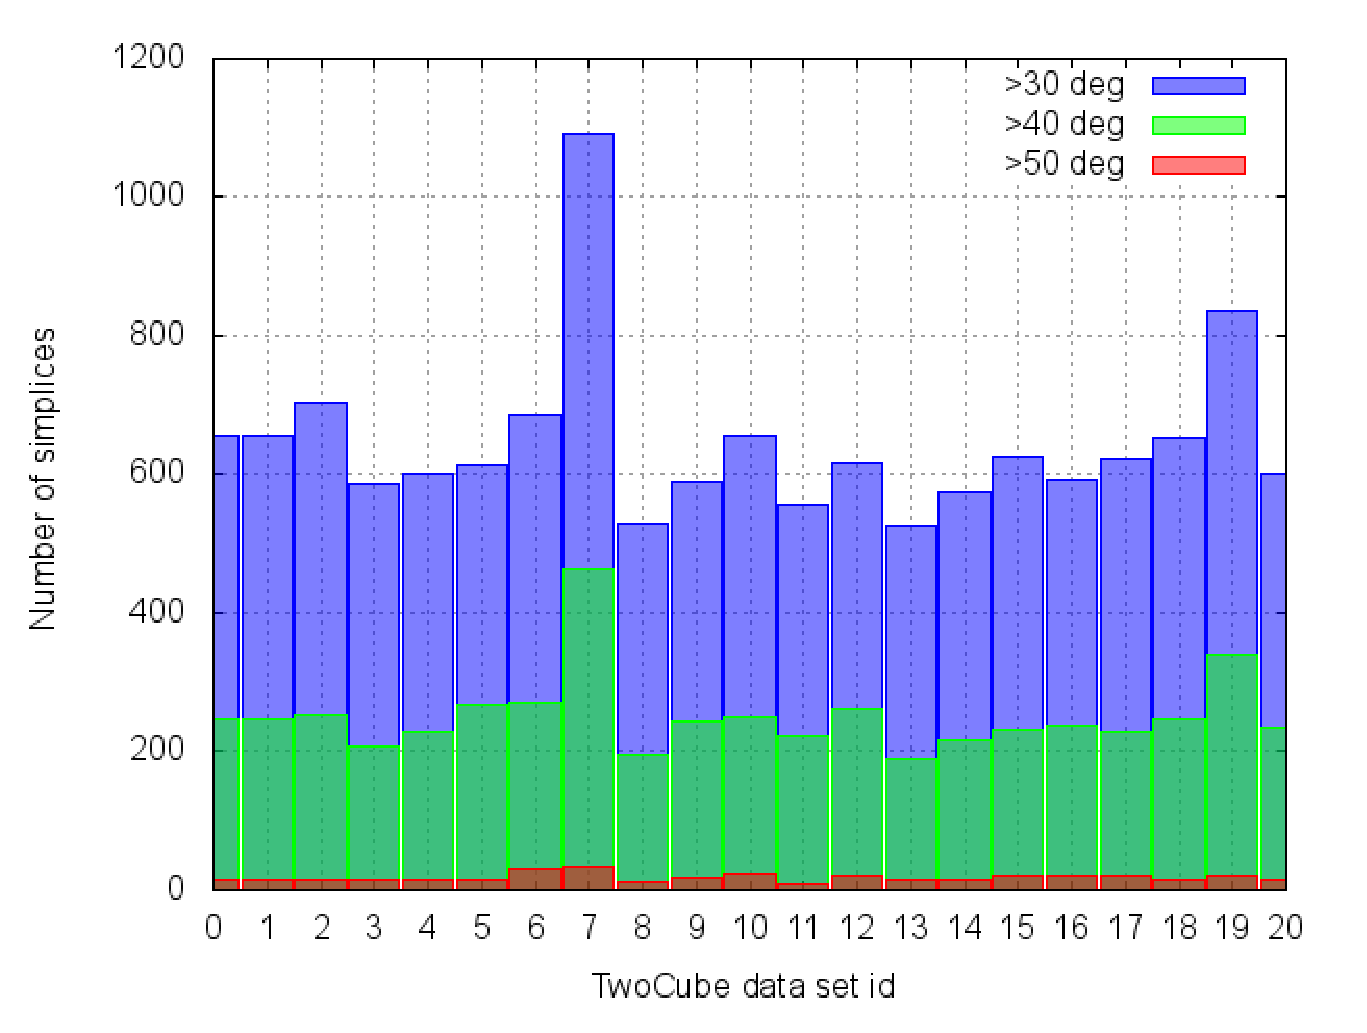
\includegraphics[width=0.6\linewidth]{images/num_simplices_large_test_twoCube.eps}\label{table:cocone_compare_with_mc_table_2}}\\
		\subfloat[]{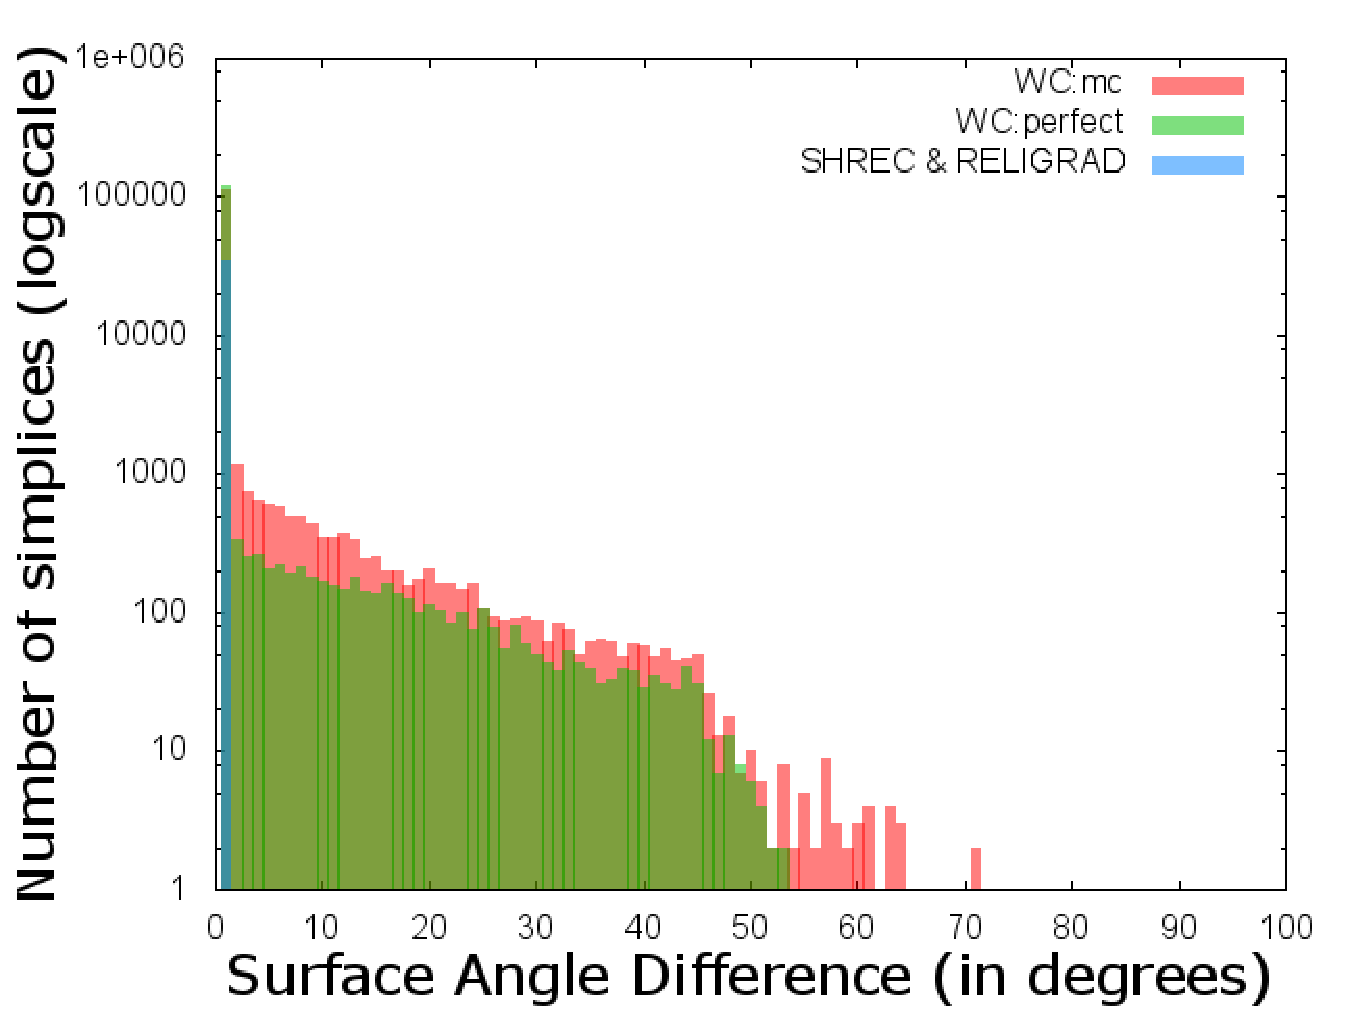
\includegraphics[width=0.6\linewidth]{images/twoCubeQuant.eps}\label{table:cocone_compare_with_mc_table_1}}
		\caption{Cocone comparison Dey et al.~\cite{Dey2012,Dey2013}. (a) Number of simplices with angle difference of 30$^\circ$, 40$^\circ$ and 50$^\circ$ from the original mesh on a subset of 21 TwoCube datasets using WeightCocone with  input points sampled from the perfect mesh. (b) Number of simplices and the corresponding angle difference to the original mesh for a single TwoCube dataset, using WeightCocone with input points super-sampled from perfect mesh, WeightCocone with input super-sampled from Marching cubes and SHREC.}
\end{figure}
\paragraph{Polymender comparison;}
We next compared SHREC to Polymender. Polymender is an implementation of mesh repairing algorithm from Ju~\cite{j-rrpm-04}. Figure~\protect\subref*{fig:polymender:b} shows the result of running Polymender on a flange dataset. Polymender creates creases, notches overlapping/degenerate triangles. On the same dataset SHREC with correct gradients and gradient computed from scalar data using RELIGRAD generates ``no" errors, Figure~\protect\subref*{fig:polymender:a} shows the corresponding result. 

We quantitatively compare the surface angle difference between the Polymender and SHREC result with the known perfect mesh. 
The results in Figure~\protect\subref*{fig:polymender:c} shows the results. Polymender produces many simplices which have large angle difference from the perfect mesh. 
\begin{figure}[tb]
	\centering
		\subfloat[]{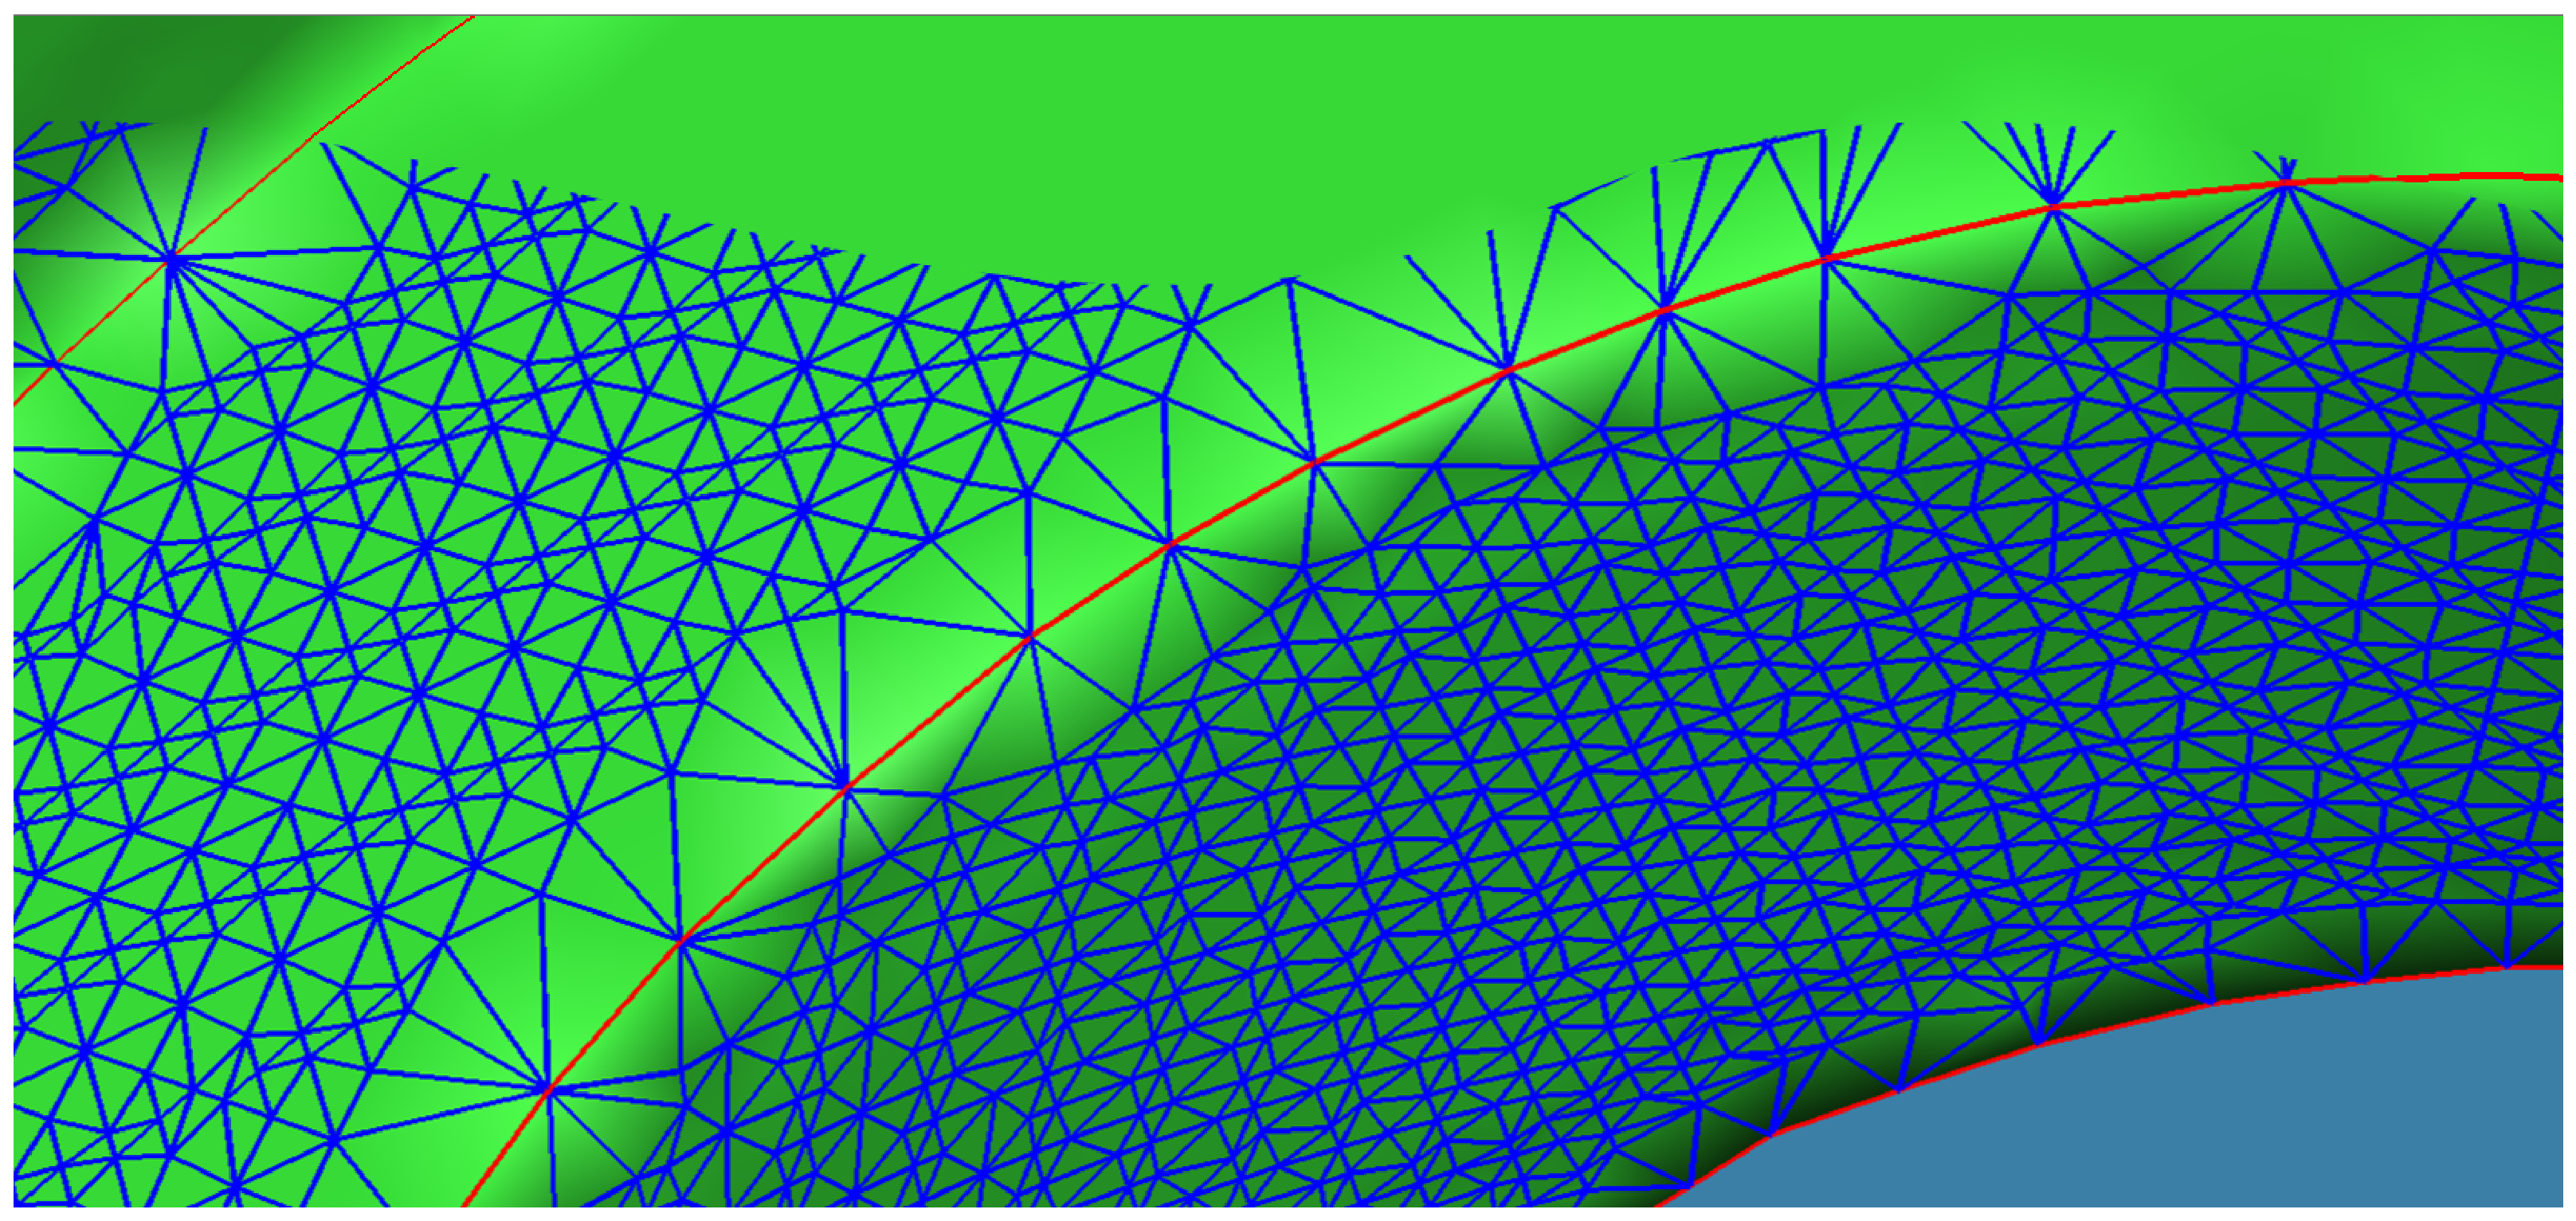
\includegraphics[width=0.45\linewidth]{images/polymender3.eps}\label{fig:polymender:a}}\quad
		\subfloat[]{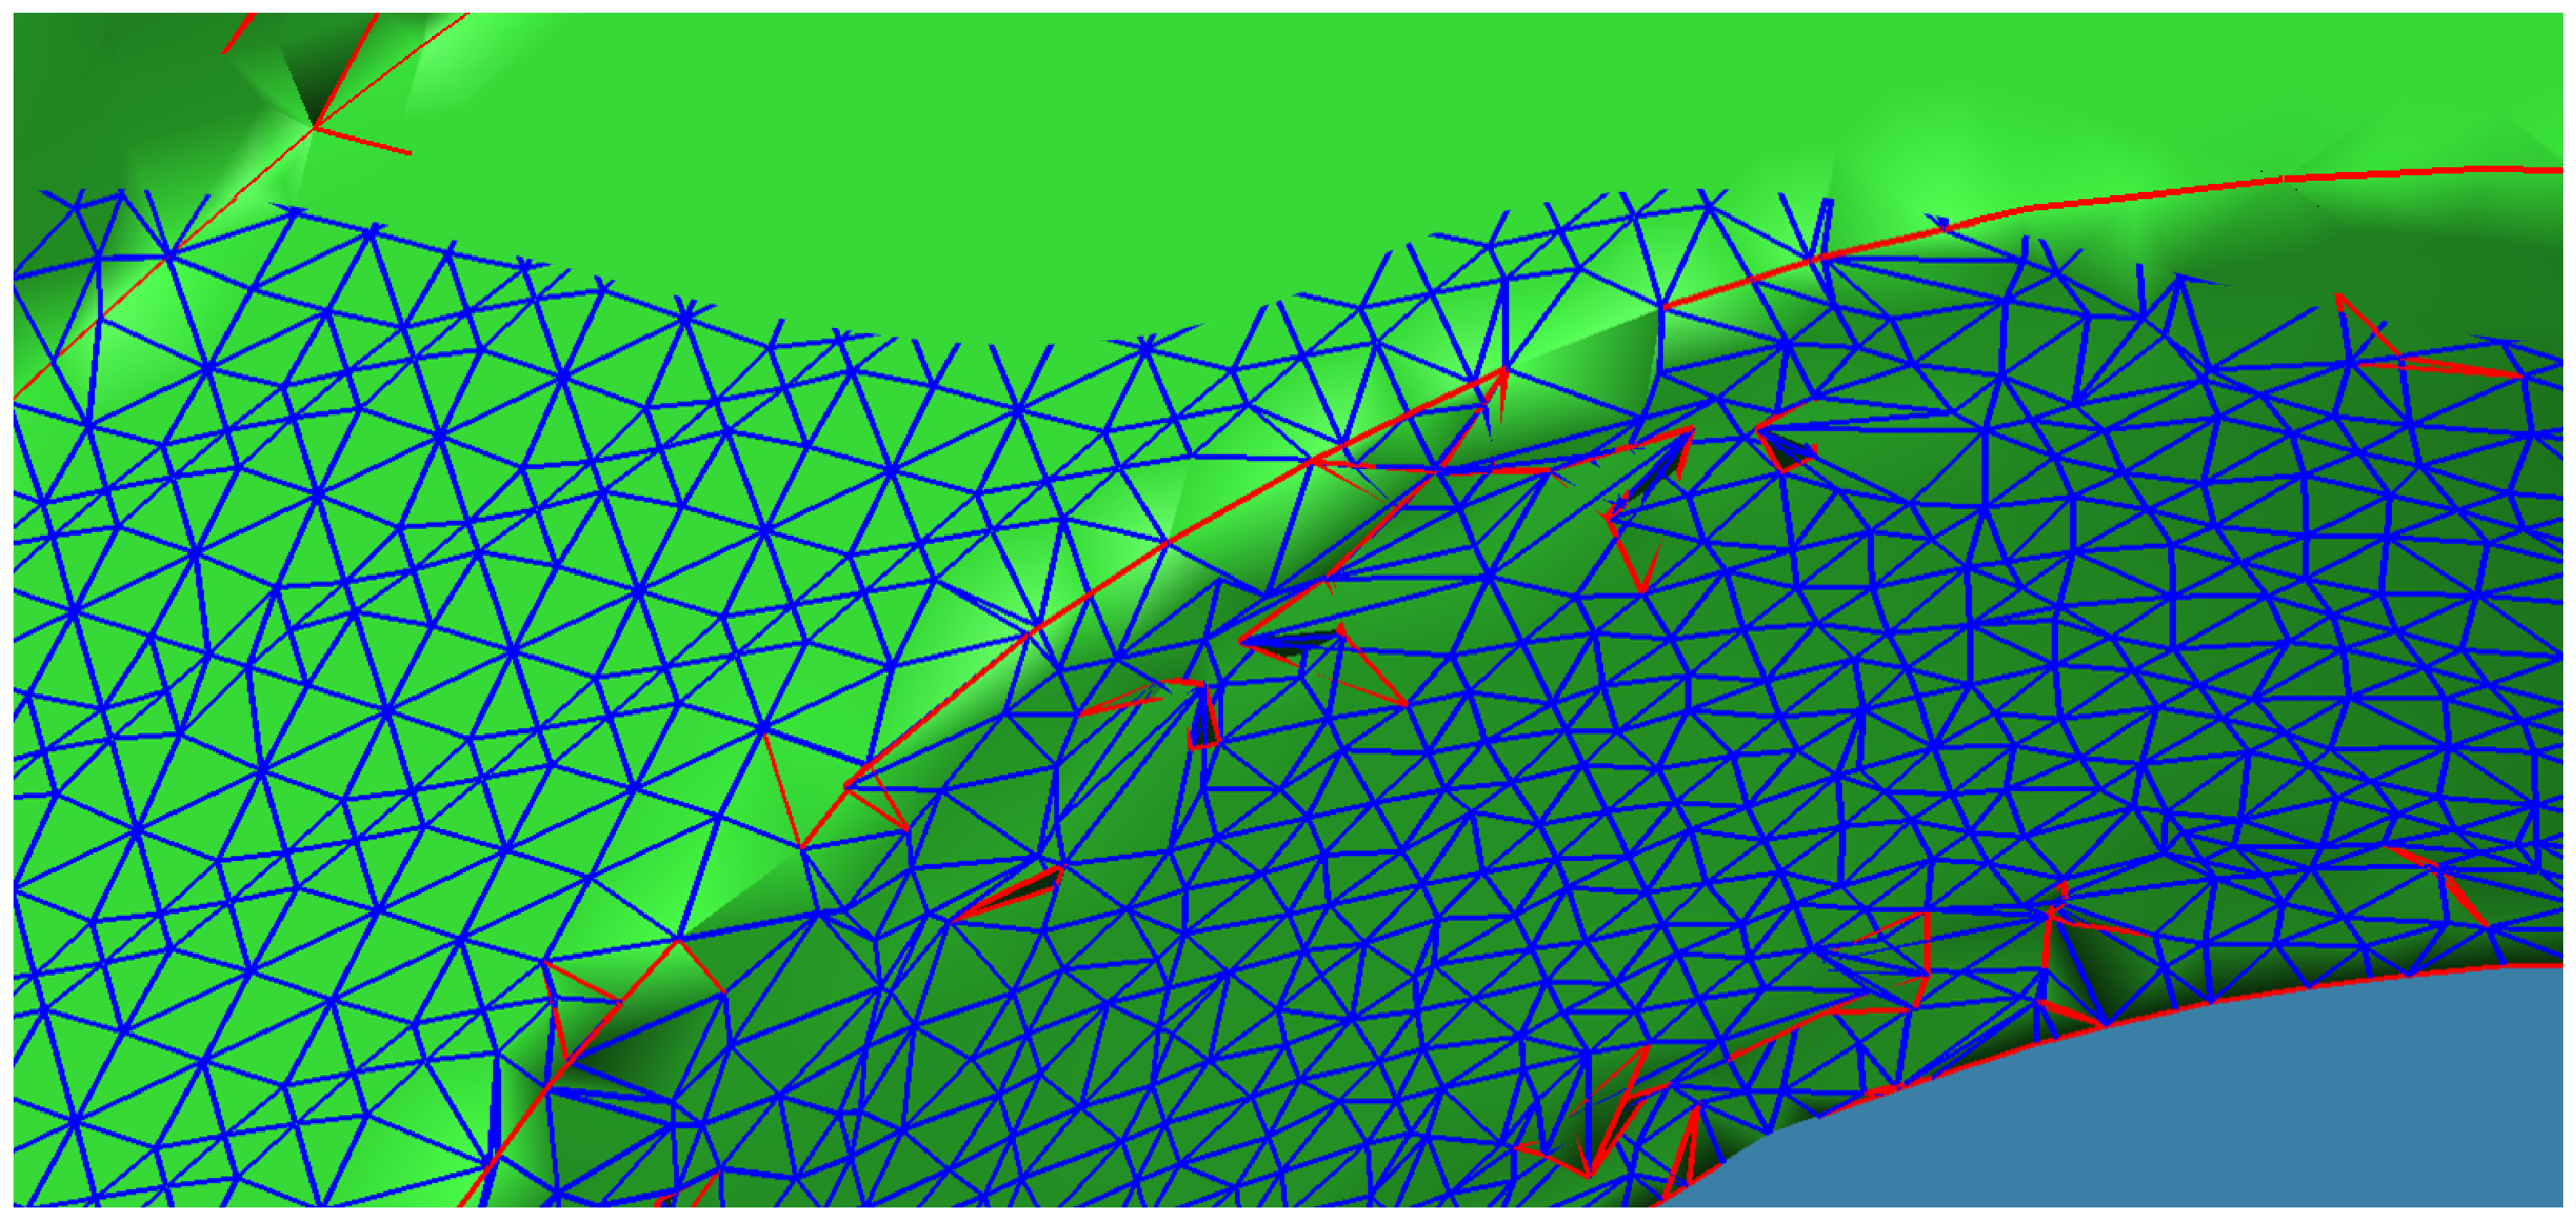
\includegraphics[width=0.45\linewidth]{images/polymender4.eps}\label{fig:polymender:b}}\\
		\subfloat[]{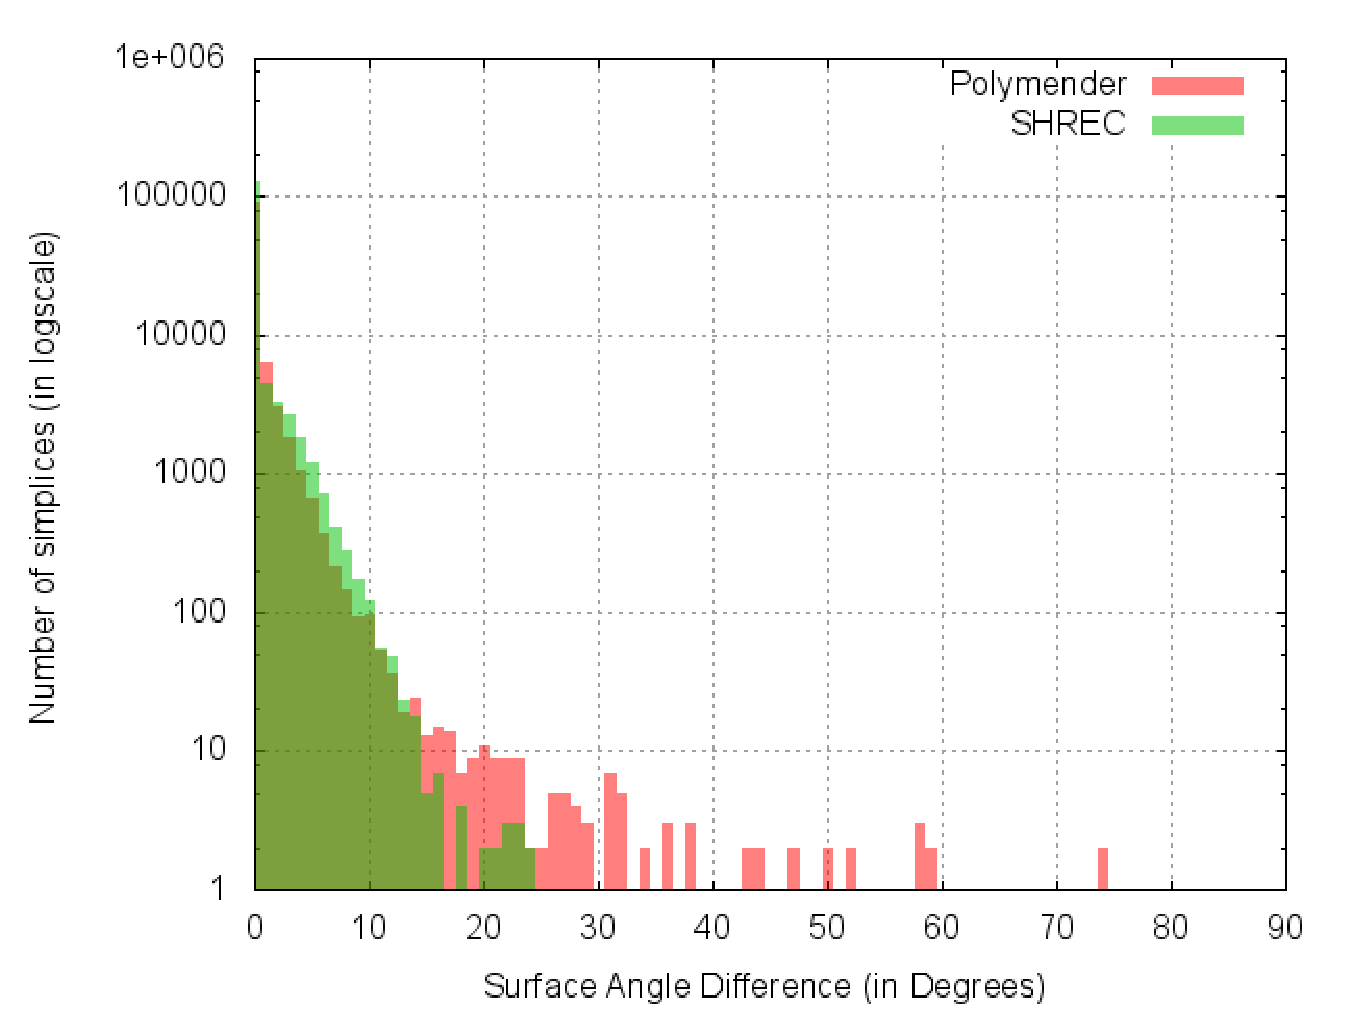
\includegraphics[width=0.7\linewidth]{images/polymenderHistogram_1.eps}\label{fig:polymender:c}}
		\caption{Comparison of Polymender with SHREC on a Flange dataset. The edges with dihedral angle less than $140^\circ$ are overlay-ed in red, a subset of the rest of the edges are overlay-ed in blue. (a) SHREC with RELIGRAD on a part of a flange dataset. (b) Polymender on the same part. (c) Surface angle distance for Polymender and SHREC results from the perfect mesh. Y-axis is in logscale. }	
\end{figure}
\paragraph{Extended Marching Cubes comparison;}
\begin{figure}[tb]
	\centering
	\subfloat[]{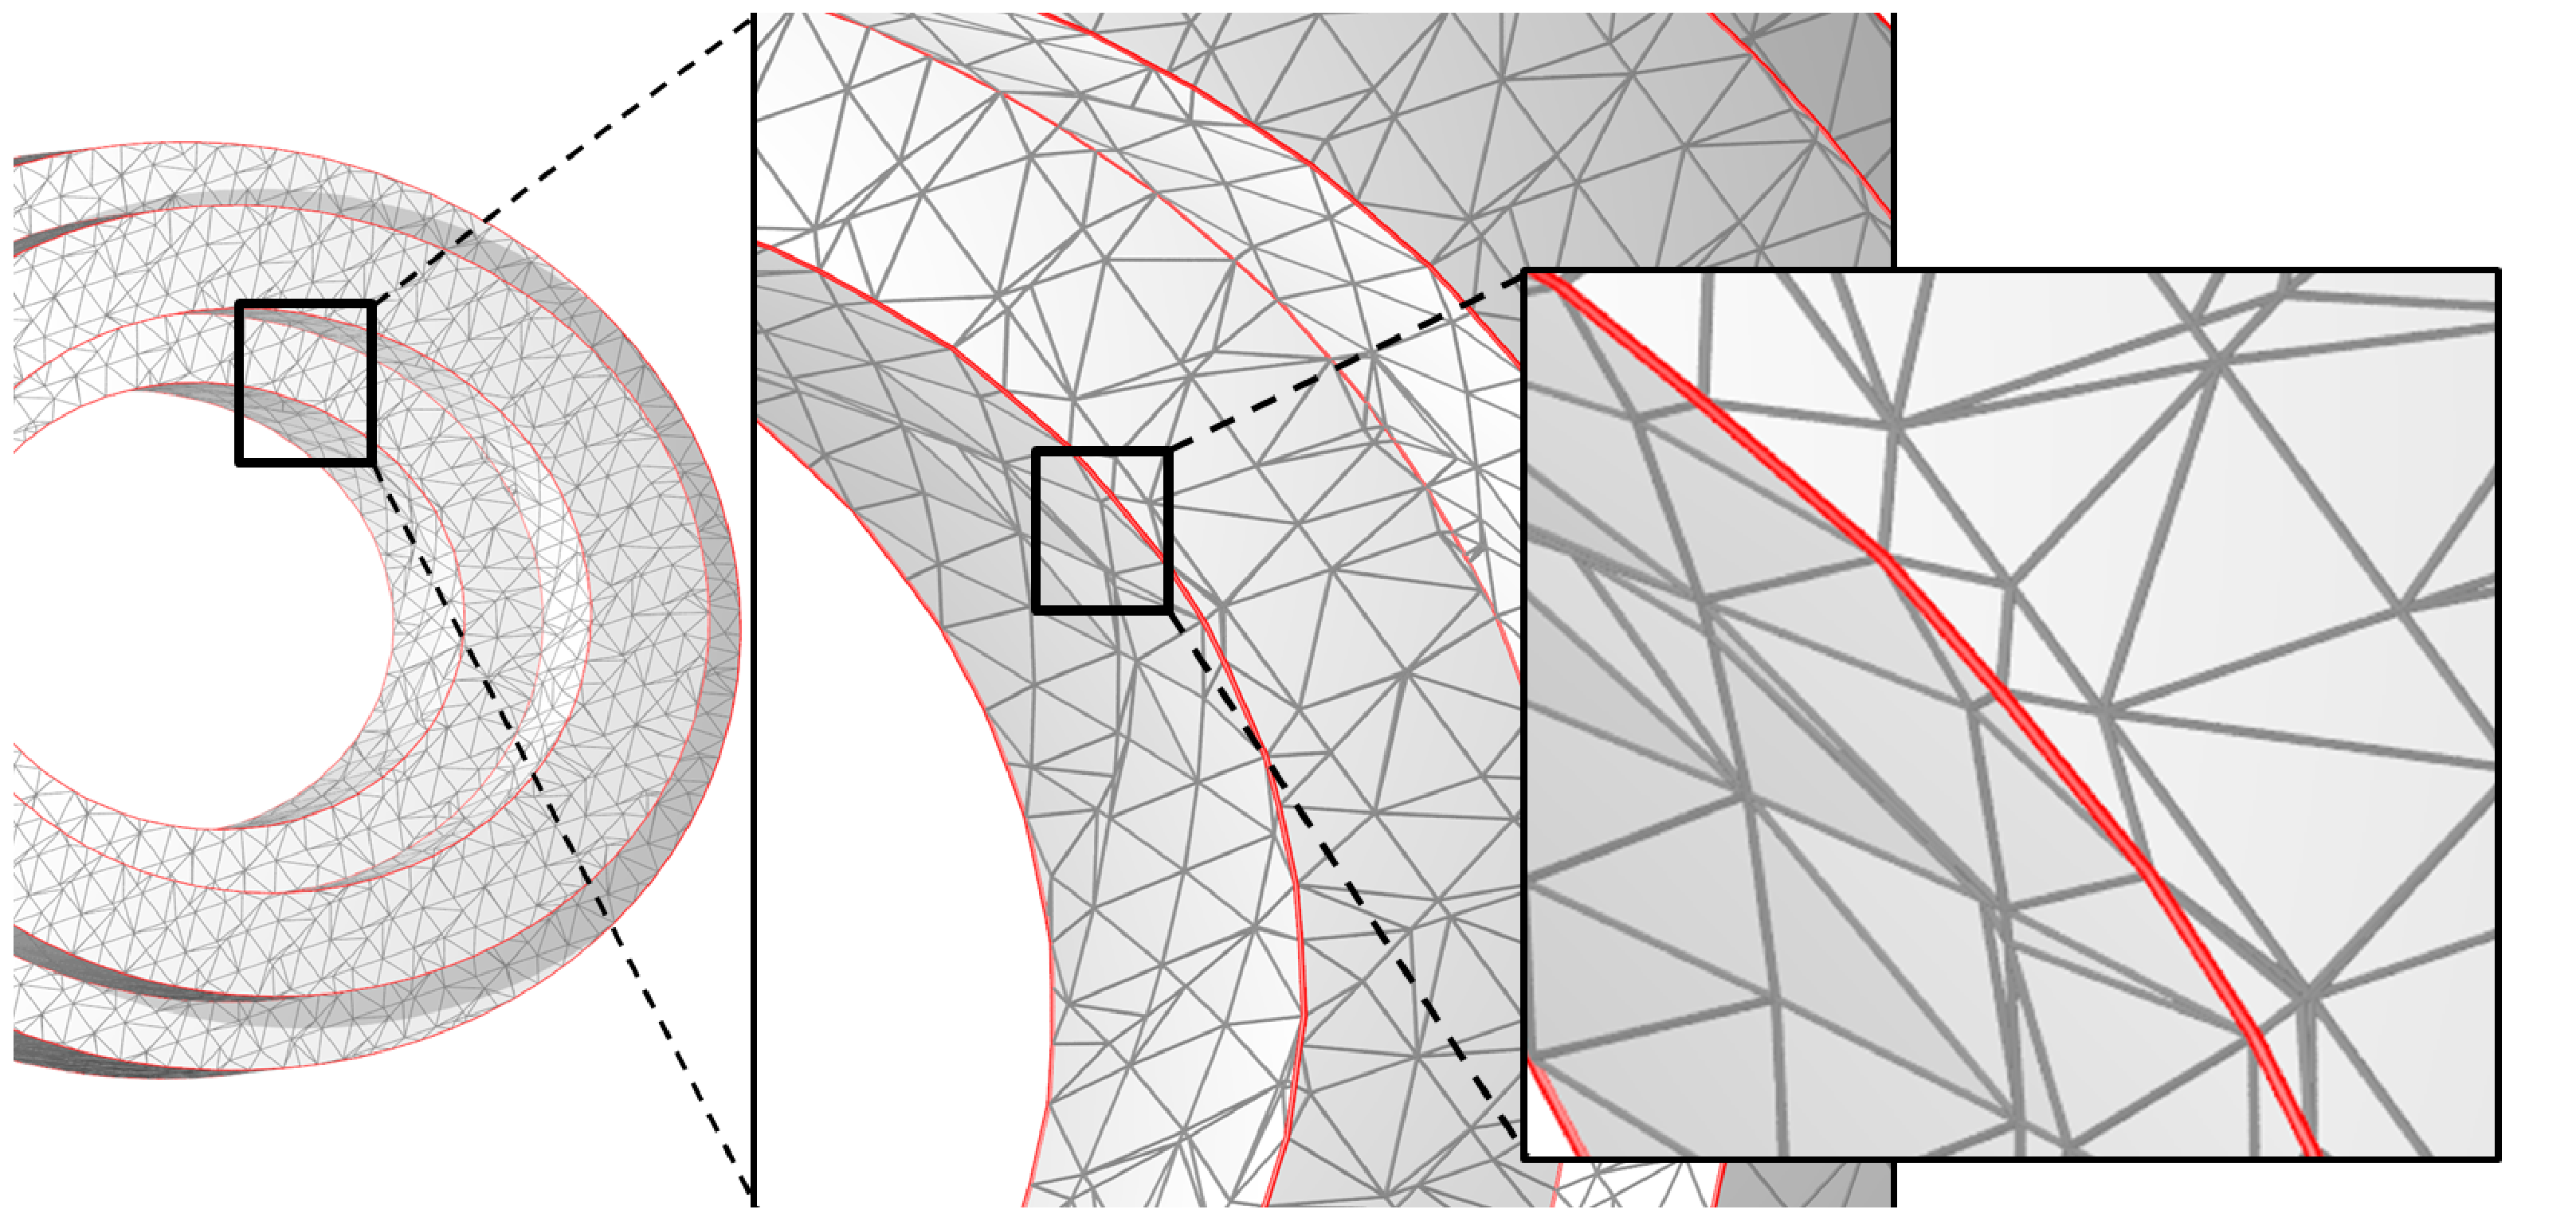
\includegraphics[width=0.7\linewidth]{images/isoExFlange.eps}\label{fig:isoEx:a}}\\
	\subfloat[]{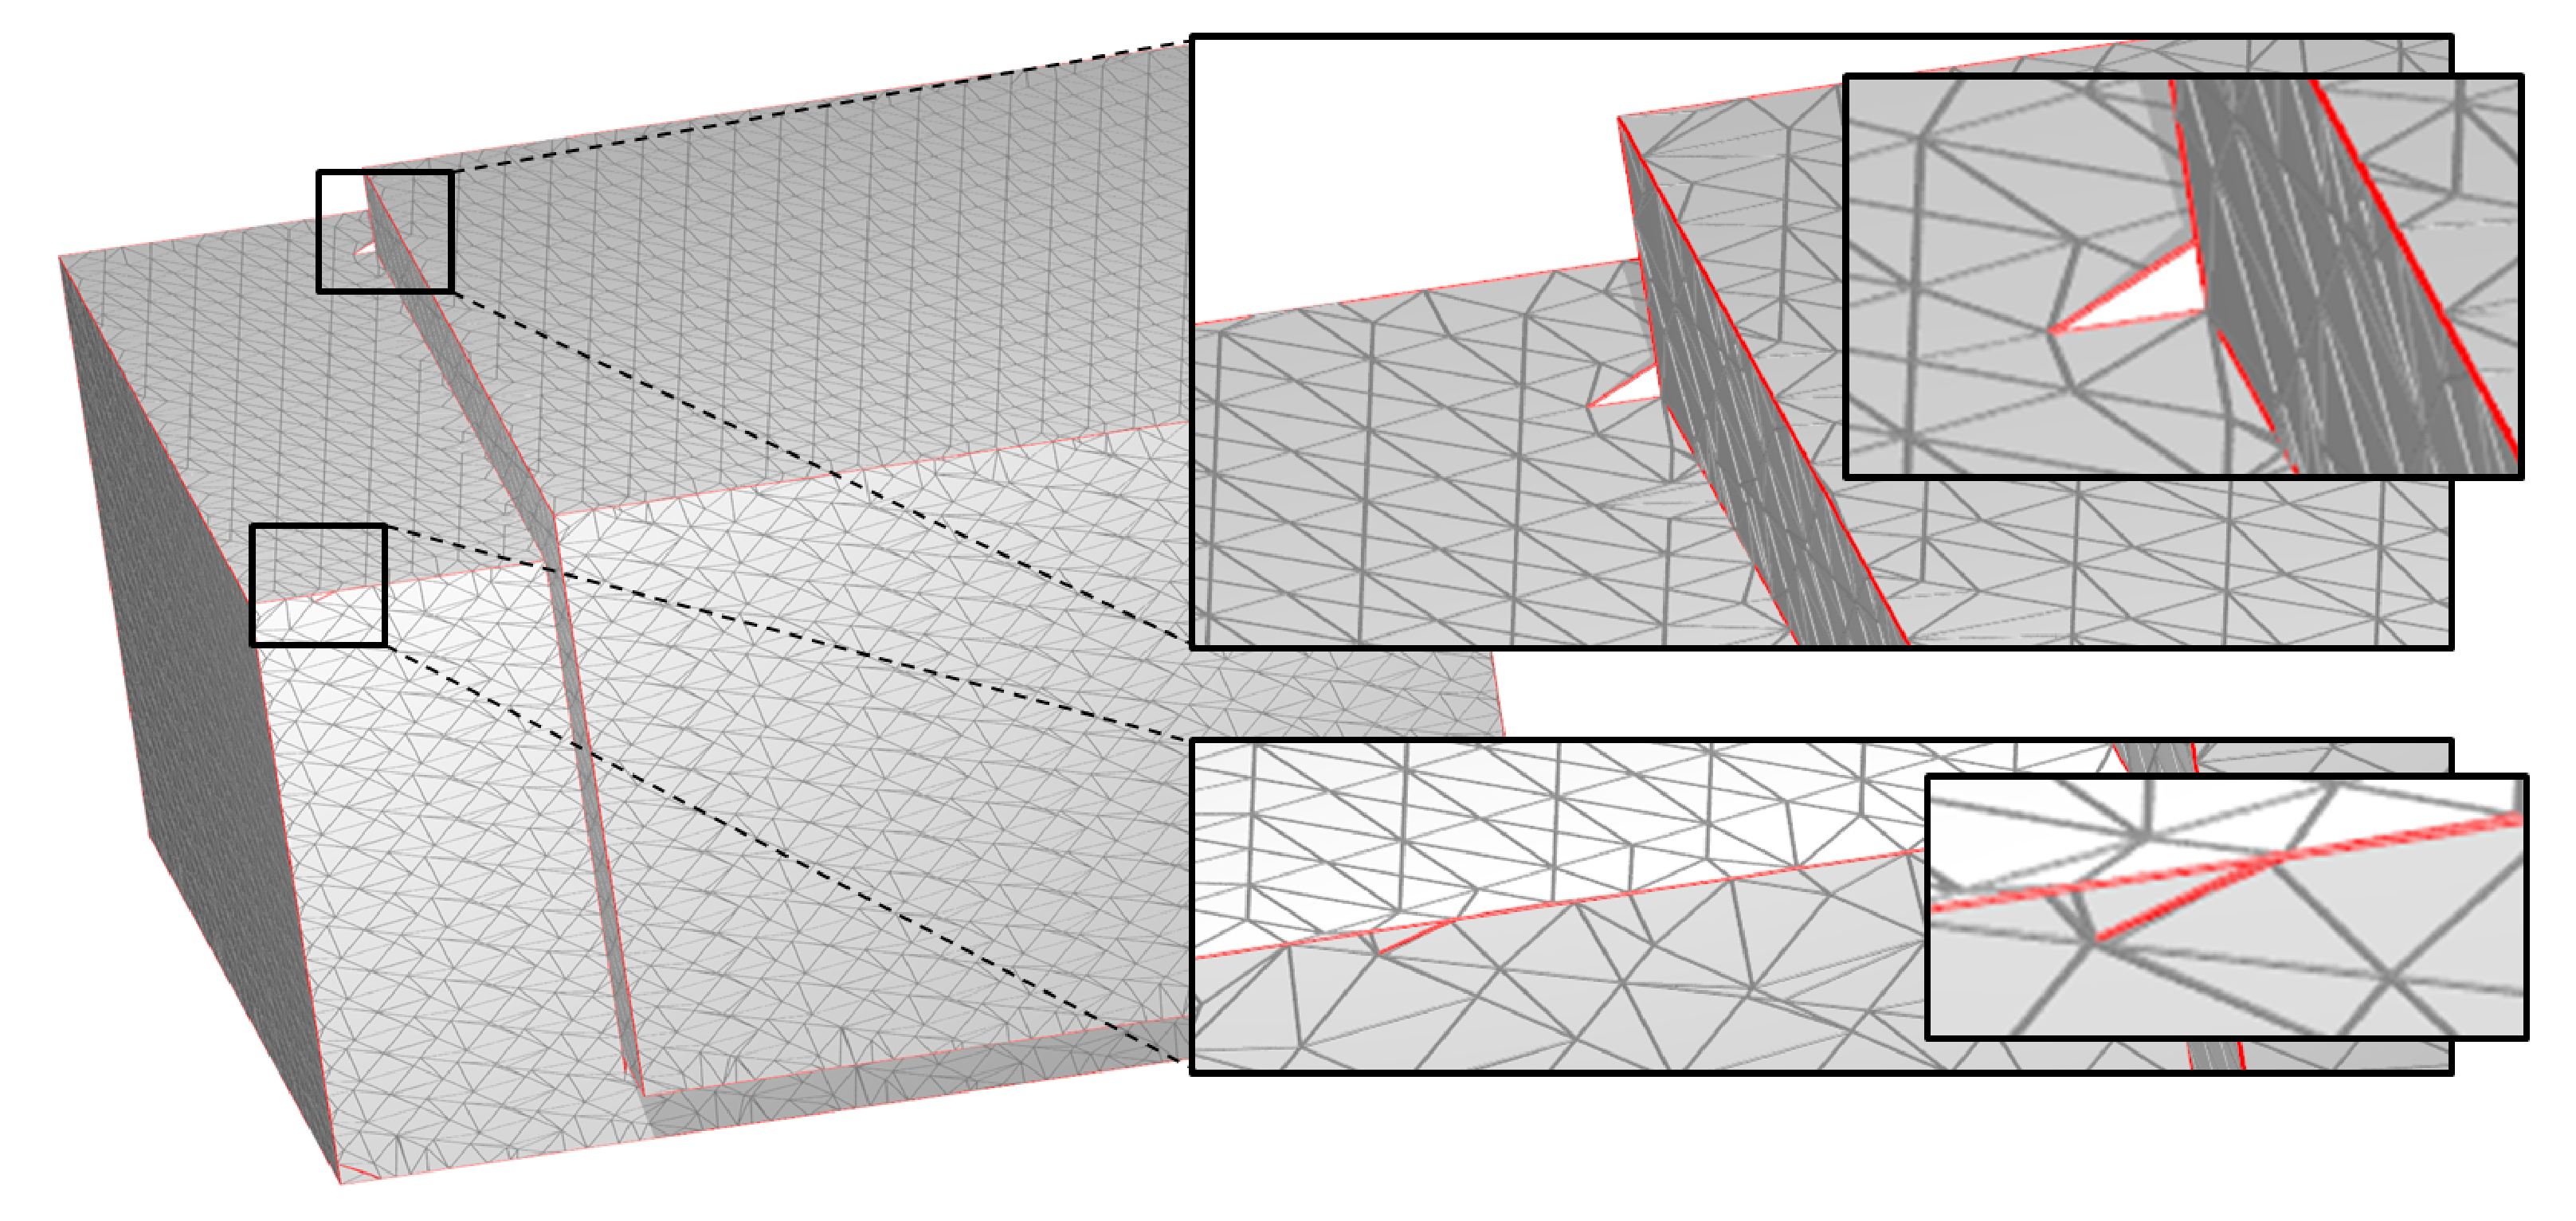
\includegraphics[width=0.7\linewidth]{images/isoExTwoCube.eps}\label{fig:isoEx:b}}
	\caption{Extended Marching Cubes results. (a) Extended Marching Cubes on a Flange dataset. (b) Extended Marching Cubes on a TwoCube dataset.}	
\end{figure}
We also compare our algorithm to Extended Marching Cubes by Kobbelt et al.~\cite{kbsh-fssev-01}. Figure~\protect\subref*{fig:isoEx:a},~\protect\subref*{fig:isoEx:b} shows the results of running Extended Marching Cubes on a Flange and a TwoCube dataset respectively. The magnified regions show that Extended Marching Cubes (same as Marching Cubes) is prone to producing small triangles. Occasionally Extended Marching Cubes also produces creases. 
\subsection{Timings}



\section{Conclusion and Future Work}
\label{section:conclusion}




\section{Acknowledgments}

We would like to thank Craig Leffel, Brent Obermiller 
and Honda of America Manufacturing
for providing the industrial CT calibration data sets.
We would like also like to thank Christoph Heinzl
from the University of Applied Sciences Upper Austria
for providing the industrial CT volt data set.



\bibliographystyle{abbrv}
\bibliography{shrec}


\appendix

\section{Closest Point under the $\Linf$ Distance}
\label{appendix:Linf}

Let $p = (p_x, p_y, p_z)$ be a point and let $L$ be a line in $\Rthree$.
We wish to find the point on $L$ closest to $p$ under the $\Linf$ distance.

Parameterize line $L$ by $t u + q$
where $u = (u_x, u_y, u_z)$ and $q = (q_x, q_y, q_z)$.
Let $q^*$ be the point of $L$ closest to $p$ under the $\Linf$ distance.
Let $\delta$ be the $\Linf$ distance from $q^*$ to $p$
and let $\cb$ be a $\gDim{2\delta}$ cube centered at $p$.
Line $L$ is tangent to $\cb$ at point $q^*$.

Let $\pi_i(p)$, $\pi_i(L)$, $\pi_i(q^*)$ and $\pi_i(\cb)$
be the projection of $p$, $L$, $q^*$ and $\cb$
onto a plane orthogonal to axis $i$.
For some axis $i$,
projected line $\pi_i(L)$ is tangent to square $\pi(\cb)$
at point $\pi_i(q^*)$.
For this axis, $\pi_i(q^*)$ is the point of $\pi_i(L)$
closest to $\pi_i(p)$ under the $\Linf$ distance.
Therefore, if $tu+q$ is the point on $L$ closest to $p$ under $\Linf$,
then $t \pi_i(u) + \pi_i(q)$ is the point 
on $\pi_i(L)$ closest to $\pi_i(p)$ under $\Linf$ for some axis $i$.
Thus, we project $p$ and $L$ onto the three planes orthogonal 
to the three axes and find $t_i$ such that $t_i \pi_i(u) + \pi_i(q)$
is closest to $\pi_i(p)$.

Consider a projection, $\pi_xy$, 
of point $p$ and line $L$ onto the $xy$ plane.
The projected point $\pi_{xy}(p)$ has coordinates $(p_x,p_y)$
and the projected line $\pi_{xy}(L)$ is parameterized 
by $t(u_x,u_y) + (q_x,q_y)$.
The point on $\pi_{xy}(L)$ which is closest to $\pi_{xy}(p)$
under the $\Linf$ distance satisfies the equation:
\begin{equation*}
|t u_x + q_x - p_x| = |t u_y + q_y - p_y|.
\end{equation*}
Equivalently,
\begin{align*}
t & = \frac{(q_y-p_y)-(q_x-p_x)}{u_x-u_y}, \mbox{ or} \\
t & = \frac{(q_y-p_y)+(q_x-p_x)}{u_x+u_y}.
\end{align*}

Solving for $t$ in each direction,
computing the $\Linf$ distance from $t u + q$ to $p$,
and taking the minimum,
identifies the point $t u + q$ which is closest to $p$
under the $\Linf$ distance.


\end{document}
